

\documentclass[12pt,a4paper]{book}



			% Packages Files
%----------------------------------%

	% Page Setttings
\usepackage[top = 1in, bottom = 1in, left = 1in, right = 1in]{geometry}

\parindent=0cm % to prevent the spacing in new paragraph or new line

\usepackage{fancyhdr}
\setlength{\headheight}{14.5pt} % needded for header and footer 

%-----------------------------------------------------------------%

\usepackage{amsmath} % needed for referencing thequation
\usepackage{amsfonts} % for maths symbols
\usepackage{graphicx}
\usepackage[export]{adjustbox}
\usepackage{nomencl} % must be loaded before caption (KOMA tocbasic conflict)
\usepackage{caption}
\usepackage{refstyle} % to reference a captioned figure


% To make hyperlinks

\usepackage[
	colorlinks=true
	,breaklinks
	]{hyperref} % needed for creating hyperlinks in the document, the option colorlinks=true gets rid of the awful boxes, breaklinks breaks lonkg links (list of figures),
	
\usepackage{xcolor}
\definecolor{c1}{rgb}{0,0,1} % blue
\definecolor{c2}{rgb}{0,0.3,0.9} % light blue
\definecolor{c3}{rgb}{0.3,0,0.9} % red blue
\hypersetup{
    linkcolor={c1}, % internal links
    citecolor={c2}, % citations
    urlcolor={c3} % external links/urls
}

	% For Code Writing
	
\usepackage{listings}

\usepackage{color}

\definecolor{mygreen}{rgb}{0 0.6 0}

\lstset{
% Set automatic Line breaking, in case we have long lines don't
% fit inside the frame or the page.
breaklines = true,
commentstyle = \color{mygreen},
breakatwhitespace = true,% don't show white space character
%numbers = left, % put line number in the code
title = \lstname
}

% ------------- For Writing Equations inisde a table and centering them ------------

\usepackage{array}

% Vertical Alignment inside the cells of the table
\newcolumntype{M}[1]{>{\centering\arraybackslash}m{#1}}

% Horizontal Alignment inside the cells of the table
\newcolumntype{P}[1]{>{\centering\arraybackslash}p{#1}}


% needed for todos liste
\usepackage{todonotes} 



% %---------- needed for long tables over pages-------
\usepackage{longtable} 

\usepackage[acronym]{glossaries}




% Macros File

% Macros Example
\def\labelaxes{Remember to include some suitable labeling for the axes and the units used in measurements.}

% 2nd way for defnining macros: the new command
% 1st parameter: name of the new command
% 2nd paramter: how many inputs this command needs, in this case only 1
% 3rd parameter: what this new command named \tbi do

\newcommand{\tbi}[1]{\textbf{\textit{#1}}}

% Command for Picture without a label

\newcommand{\pic}[3]{\begin{figure}[h]
\centering
\includegraphics[width = 0.7\textwidth, frame]{#1}
\caption{#2}
\end{figure}}








\DeclareMathOperator*{\argmax}{argmax} % thin space, limits underneath in displays

\DeclareMathOperator*{\argmin}{argmin}

\title{Signal Processing}
\author{Ranim Tom}



\begin{document}

% downloaded template
%\input{content/title_page_1} 

\maketitle



\chapter*{Abstract}

This document represents a \tbi{course reader} for digital signal processing work. 

Mainly it contains:

\begin{itemize}

\item theoratical explanation

\item proofs for theorems

\item worked examples

\end{itemize}


Simulation (via programming, or \verb|GNU| radio) validating the theory are presented in a separate document.\\

\underline{Prerequiste:} a course in signal and system is assumed to be taken, since I will focus on DSP aspect and practical consideration.


\tableofcontents


\pagestyle{fancy}
\fancyhf{} % Clear header and footer
\rhead{\rightmark}
\lhead{Chapter \thechapter}
\rfoot{Page \thepage}

\chapter{Introduction to Digital Signal Processing}

\underline{Notes:}\\

\begin{itemize}

\item In DSP, all the processing is done in the discrete domain

\item Advantage of DSP over the analog domain:

Suppose we have a system which suffers from noise, and we want to eliminate this noise. We could use some analog filter (form capacitors and inductors) and filter this noise at the unwanted frequency.\\

Now, some day it becomes hot, and our filter start to play due to the hot temperature, so we need to change the filter and the hardware.\\

However in the digital domain, it's all about the software and the implementation, we could only change the filter coefficient and keep the same hardware.

\end{itemize}


%**************************************************
%**************************************************
%**************************************************




\chapter{Sampling}


\section{References}

This chapter is mainly taken from \cite{signal_processing_Lathi}.

\section{Introduction to Sampling and Reconstruction}

Sampling is a common operation in signal processing, since our computers and hardware we use process \tbi{discrete sample}. An example is shown in \autoref{fig:Sampling:Sampling_Example}.


\begin{figure}[h]
\centering
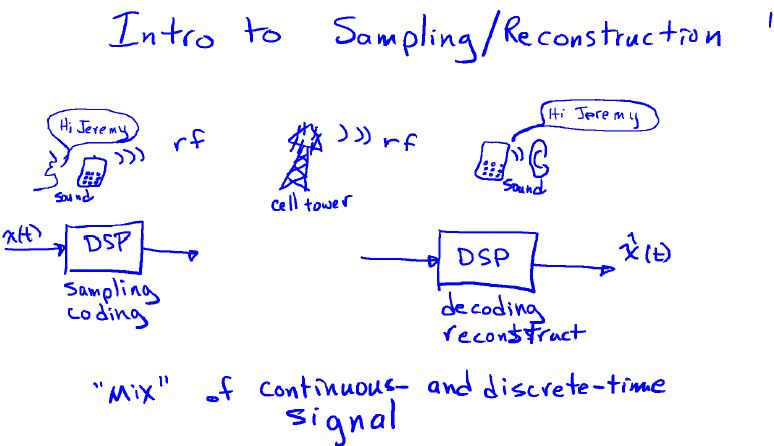
\includegraphics[width = 0.7\textwidth, frame]{Figures/Sampling/Sampling_Example}
\caption{Example of Sampling: digital transmission}
\label{fig:Sampling:Sampling_Example}
\end{figure}

\begin{itemize}

\item We have some sound denoted by $x(t)$

\item Inside the phone, there is some DSP chip which do the sampling and the coding process

\item Then some hardware to modulate the signal to transform it into RF signal for transmission

\item At the receiver, the signal is demodulated back to the base band status

\item Then a decoding and reconstruction process is done to reconstruct the original signal $x(t)$.

\end{itemize}

The goal is that we hope that $\hat{x}(t) \, \approx \, x(t)$.\\

We will use the Fourier transform to analyze the effect of sampling and tackle the problem of reconstruction, and also we ask several question to build an efficient system which can do this reconstruction:

\begin{itemize}
\item How fast do we need to sample ?

\item How to reconstruct ?
\end{itemize}


\section{Sampling Continuous Time Signals}
\label{Sec:Sampling:Sampling_Continuous_Time_Signals}



\subsection{Impulse Sampling Analysis using Fourier Transform}

To do the mathematical derivation later.

\subsection{Intuition and Interpretation}

\begin{figure}[h]
\centering
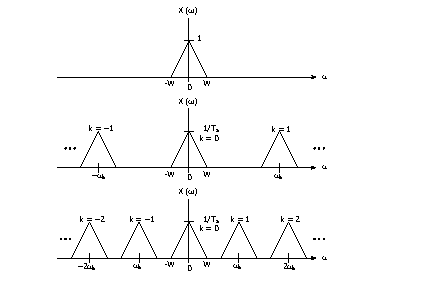
\includegraphics[width = 0.7\textwidth, frame]{Figures/Sampling/impulse_sampling_spectrum_1}
\caption{Sampling Higher then the Nyquite Rate}
\label{fig:Sampling:impulse_sampling_spectrum_1}
\end{figure}

\begin{itemize}
\item When sampling higher then the Nyquist rate, we could still distinguish the original version of the spectrum, which is in the middle
\end{itemize}


\newpage
Let's try now to decrease the sampling rate ($\omega_s$ decrease) as shown in \autoref{fig:Sampling:impulse_sampling_spectrum_2}.


\begin{figure}[h]
\centering
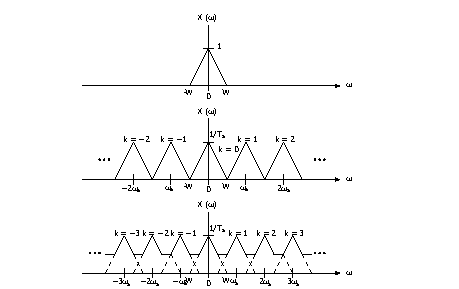
\includegraphics[width = 0.7\textwidth, frame]{Figures/Sampling/impulse_sampling_spectrum_2}
\caption{Decreasing the Nyquist Rate: Aliasing Result}
\label{fig:Sampling:impulse_sampling_spectrum_2}
\end{figure}

\begin{itemize}

\item When decreasing the sampling rate $\omega_s$, the shifted spectrum get close to each other

	\begin{itemize}
	\item In the $\mathrm{2}^\mathrm{nd}$ row of \autoref{fig:Sampling:impulse_sampling_spectrum_2}, we are sampling exactly at the Nyquist rate
	
	\item No gap between the original spectrum and the shifted version
	\end{itemize}


\item When sampling rate $\omega_s$ less then the \tbi{Nyquist rate}, the shifted versions have collide with the original spectrum 

	\begin{itemize}
	\item The only thing we can see is the blue solid line
	
	\item We could not retrieve the original spectrum as before now.
	\end{itemize}

\end{itemize}



\subsection{Example: Sampling a Cosine}

Let's take the signal $x(t) \, = \, \text{cos}\left( \pi t \right)$, and sample this signal at different sampling rate $\omega_s$ and study the effect for different values of $\omega_s$.

\begin{figure}[h]
\centering
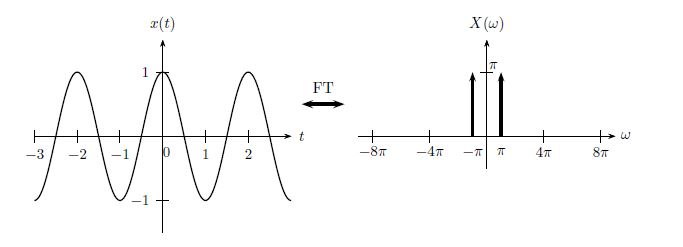
\includegraphics[width = 0.7\textwidth, frame]{Figures/Sampling/Sampling_cosine}
\caption{Example of Sampling a cos: period $\, = \, 2$ s}
\label{fig:Sampling:Sampling_cosine}
\end{figure}


\newpage
First case we take $\omega_s \, = \, 8 \pi \rightarrow \, T_s \, = \, \displaystyle\frac{1}{4}$s. Case is shown in \autoref{fig:Sampling:Sampling_cosine_2}.

 
\begin{figure}[h]
\centering
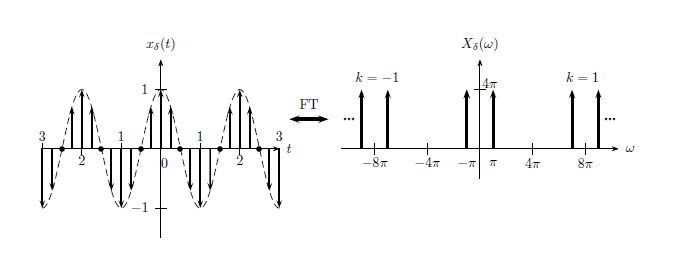
\includegraphics[width = 0.7\textwidth, frame]{Figures/Sampling/Sampling_cosine_2}
\caption{$\omega_s \, = \, 8 \pi \, ; \, T_s \, = \, \displaystyle\frac{1}{4}$ s}
\label{fig:Sampling:Sampling_cosine_2}
\end{figure}

	\begin{itemize}
	\item The shifted spectrum are repeated at multiple of $\omega_s$
	
	\item Don't forget that we have the scale factor $\displaystyle\frac{1}{T_s} \, = \, 4$
	\end{itemize}
	
Case 2 shown in \autoref{fig:Sampling:Sampling_cosine_3}: we decrease $\omega_s$ to become $2\pi \rightarrow \, T_s \, = \, 1$s. So we take less samples per second.

\begin{figure}[h]
\centering
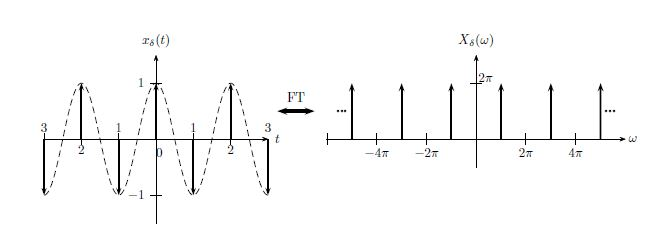
\includegraphics[width = 0.7\textwidth, frame]{Figures/Sampling/Sampling_cosine_3}
\caption{Exactly Sampling at Nyquist rate ; $\omega_s \, = \, 2 \pi \, ; \, T_s \, = \, 1$ s}
\label{fig:Sampling:Sampling_cosine_3}
\end{figure}

\begin{itemize}
\item The case shown in \autoref{fig:Sampling:Sampling_cosine_3}: we are sampling \tbi{exactly at the Nyquist rate} where $\omega_s \, = \, 2 W$ and $W \, = \, \pi$.

\item We are still able to see the original spectrum located at $\pi$ and $-\pi$

\item However notice that at the scaling factor: it is true that $\displaystyle\frac{1}{T_s} \, = \, 1$, but we have $2 \pi$

	\begin{itemize}
	
	\item This is because when we shift the original spectrum at multiple of $\omega_s$, the dirac shifted land on top of the original dirac , and added together	
	
	\end{itemize}

\end{itemize}

\newpage
Last case shown in \autoref{fig:Sampling:Sampling_cosine_4} is we sample below Nyquist rate and aliasing effect occur also.


\begin{figure}[h]
\centering
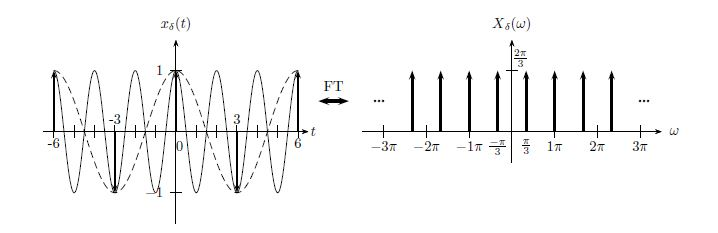
\includegraphics[width = 0.7\textwidth, frame]{Figures/Sampling/Sampling_cosine_4}
\caption{Sampling below Nyquist rate ; $\omega_s \, = \displaystyle\frac{2 \pi}{3} \, ; \, T_s \, = \, 3$ s}
\label{fig:Sampling:Sampling_cosine_4}
\end{figure}


\begin{itemize}

\item Because we are sampling below the Nyquist rate, the reconstructed cosine appear to be a low frequency one

\item This is can be deduced from the frequency spectrum: notice that when the spectrum is shifted at multiple of $\omega_s \, = \, \displaystyle\frac{2 \pi}{3}$, 

	\begin{itemize}
	
	\item the dirac component located at $-\pi$ (this is the original one) is shifted to $\displaystyle\frac{-\pi}{3}$	
	
		\item Same for the dirac component located at $+\pi$ (this is also the original one) is shifted to $\displaystyle\frac{+\pi}{3}$
		
		\item So it seems that the original spectrum is located at $\left[\, \displaystyle\frac{-\pi}{3} \, ; \, \displaystyle\frac{+\pi}{3} \, \right]$
	
	\end{itemize}

\end{itemize}


\subsection{Predicting Aliasing frequency}

We have seen in \autoref{fig:Sampling:Sampling_cosine_4} that when we sample below the Nyquist rate, aliasing occurred and the cos signal has transformed from high frequency $f \, = \, \displaystyle\frac{1}{2}$ Hz to $f_{\text{alias}} \, = \, \displaystyle\frac{1}{3}$ Hz. In this section we try to use some equations in order to predict in advance the aliasing frequency $f_{\text{alias}}$.\\

The equation are:

\begin{equation}
\begin{array}{rcl}
f_{\text{alias}} \, &\leq& \, \displaystyle\frac{Fs}{2} \\
f_{\text{alias}} \, &=& \, \lvert f_{\text{original}} \, - \, m \, f_s  \rvert \quad \text{where } m \, = \, 0 \, ; \, 1 \, ; \, 2 ;\, \cdots
\end{array}
\label{Eq:Sampling:alias_frequency}
\end{equation} 

\newpage
An example is shown in \autoref{fig:Sampling:alias_frequency}.

\begin{figure}[h]
\centering
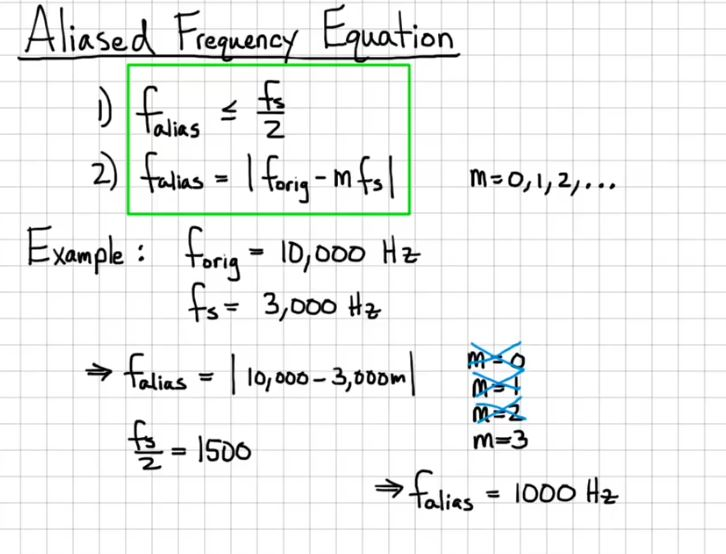
\includegraphics[width = 0.7\textwidth, frame]{Figures/Sampling/alias_frequency}
\caption{Predicting alias frequency}
\label{fig:Sampling:alias_frequency}
\end{figure}

\begin{itemize}

\item We have some signal where $f_{\text{original}} \, = \, 10^4$ Hz

\item We sample the signal with $f_s \, = \, 3000$ Hz

	\begin{itemize}
	\item Clearly, aliasing will occur since we dind't respect the Nyquist condition
	\end{itemize}


\item We keep using \ref{Eq:Sampling:alias_frequency}:

	\begin{itemize}
	
	\item We solve for $m \, = \,0$, we obtain $f_{\text{alias}} \, = \, 10^4$. This $f_{\text{alias}}$ doesn't satisfy the condition $f_{\text{alias}} \, \leq \, \displaystyle\frac{Fs}{2} $, so we keep solving for other value of $m$.
	
	
	\item For $m \, = \, 3$, we get $f_{\text{alias}} \, = \, 10000$ Hz, and this frequency satisfy the condition $f_{\text{alias}} \, = \, 1000 \, \text{Hz} \, \leq \, \displaystyle\frac{Fs}{2} $ 
	
	\end{itemize}

\end{itemize}

So when we sample a signal of $f_{\text{original}} \, = \, 10^4$ Hz with $f_s \, = \, 3000$ Hz, we get an alias frequency of 1000 Hz.


\newpage
\section{Examples}

Consider the analog signal: $x(t) \, = \, 4 \, + \, 2\, \text{cos}\left(\, 150 \pi t \, + \, \displaystyle\frac{\pi}{3} \,\right) \, + \, 4 \, \text{sin}\left(\, 350 \pi t \,\right)$.\\

To be done later.


\section{Other Practical Considerations}

In this section we look to more sophisticated points related to sampling, like the fact that in \tbi{real world signals}, they are always time limited, and the implication of this time limitation on sampling. Also we deals with several \tbi{application to sampling} like pulse modulation,$\cdots$.

\subsection{Time Limited Signals}

The time-bandwidth product also know as \tbi{uncertainty principle} is shown in equation (\ref{Eq:time_band_produc}) 

\begin{equation}
\begin{array}{rcl}
T_d \, &=& \, \left[ \displaystyle\frac{\int\limits_{-\infty}^{+\infty}  t^2 \, |x(t)|^2 \, dt}{\int\limits_{-\infty}^{+\infty} |x(t)|^2 \, dt} \right]^{0.5} \\ \\
B_w \, &=& \, \left[ \displaystyle\frac{\int\limits_{-\infty}^{+\infty}  \omega^2 \, |X(\omega)|^2 \, d\omega}{\int\limits_{-\infty}^{+\infty} X|(\omega)|^2  \, d\omega} \right]^{0.5} \\ \\
T_d \, \times \, B_{\omega} \, &\geq& \, 0.5
\end{array}
\label{Eq:time_band_produc}
\end{equation}

Equation (\ref{Eq:time_band_produc}) says that if we have a \tbi{time limited signal} , the \tbi{frequency content} of the signal will \tbi{extent to infinity}, and hence this will cause a \tbi{problem when doing sampling}. Sampling theorem tell us that we need to sample at the Nyquist rate $F_s$ where $F_s$ is at least 2 times higher than the maximum frequency of the signal. Since the maximum frequency is infinity, we can't sample at infinity, and \tbi{this cause any frequency content above $\displaystyle\frac{F_s}{2}$ to fold with the original spectrum}. 


\newpage
This is illustrated in \autoref{fig:Sampling:Folding}.


\begin{figure}[h]
\centering
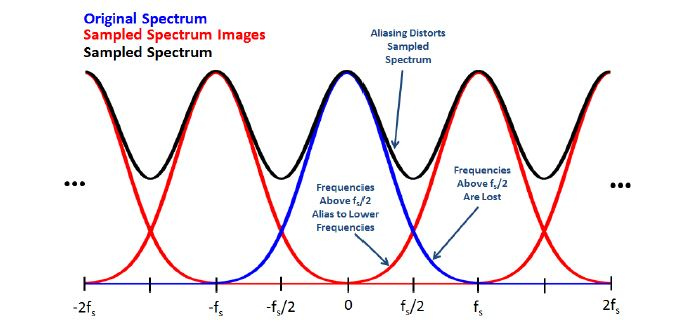
\includegraphics[width = 0.7\textwidth, frame]{Figures/Sampling/Folding}
\caption{Signal Aliasing: frequency at $\displaystyle\frac{F_s}{2} \, + \, f_x$ shows at $\displaystyle\frac{F_s}{2} \, - \, f_x$}
\label{fig:Sampling:Folding}
\end{figure}

\begin{itemize}

\item We have the original theoretical spectrum in blue we wish to recover

\item We know from sampling theorem that due to sampling, the spectrum will get replicated at multiple of $F_s$, and the resultant spectrum will be the summation of all the copies at every point, which give us the black spectrum.

\end{itemize}

Now when we wish to recover the spectrum (the blue one in  \autoref{fig:Sampling:Folding}), we apply the ideal reconstruction by cutting above $\displaystyle\frac{F_s}{2}$ and below $- \displaystyle\frac{F_s}{2}$ as shown in \autoref{fig:Sampling:Folding_reconstruction}.



\begin{figure}[h]
\centering
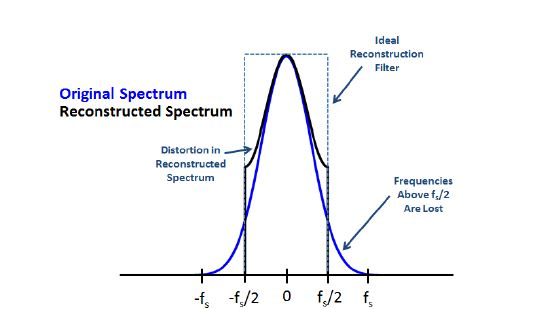
\includegraphics[width = 0.7\textwidth, frame]{Figures/Sampling/Folding_reconstruction}
\caption{Reconstructed Signal is Distorted}
\label{fig:Sampling:Folding_reconstruction}
\end{figure}

However, instead of getting back to the blue (original one), we end up with the black one. The black spectrum contains \tbi{2 type of distortion}:

\begin{enumerate}

\item Distortion due to folding (aliasing): the black amplitude values are the result from the summation of frequencies above and below $\pm\, \displaystyle\frac{F_s}{2}$, which fold back in the interval $\left[\, -\, \displaystyle\frac{F_s}{2} \, ; \, + \, \displaystyle\frac{F_s}{2} \, \right]$

\item Distortion due to the loss of high frequency content: the original blue spectrum does indeed have high frequency content above $\displaystyle\frac{F_s}{2}$ due to the uncertainty principle.

\end{enumerate}

\subsection{Anti-Aliasing Filter}

How can we fight the distortions introduced in \autoref{fig:Sampling:Folding_reconstruction}? \\

First let's talk about the aliasing distortion. We know that frequencies above $\displaystyle\frac{F_s}{2}$ will fold back to the original spectrum (as discussed in \autoref{fig:Sampling:Folding}), so what we can do is get off the frequencies above $\displaystyle\frac{F_s}{2}$ so they won't fold back when doing the reconstruction. In other words, we are limiting the signal to what it's called \tbi{effective bandwidth} when doing the cutting. Process is shown in \autoref{fig:Sampling:Anti_Aliasing_Filter}.

\begin{figure}[h]
\centering
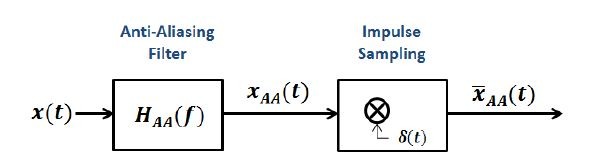
\includegraphics[width = 0.7\textwidth, frame]{Figures/Sampling/Anti_Aliasing_Filter}
\caption{Anti Aliasing Filter}
\label{fig:Sampling:Anti_Aliasing_Filter}
\end{figure}

\begin{itemize}

\item We have some time limited signal $x(t)$

\item We apply the anti-aliasing filter

\item Then we do impulse sampling

\end{itemize}

Result of this process is shown in \autoref{fig:Sampling:Anti_Aliasing_Filter_Result}.

\begin{figure}[h]
\centering
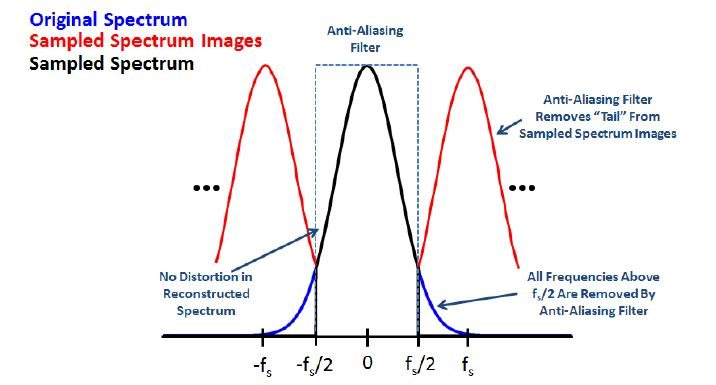
\includegraphics[width = 0.7\textwidth, frame]{Figures/Sampling/Anti_Aliasing_Filter_Result}
\caption{Anti Aliasing Filter: no folding frequencies}
\label{fig:Sampling:Anti_Aliasing_Filter_Result}
\end{figure}

\begin{itemize}

\item If we compare \autoref{fig:Sampling:Anti_Aliasing_Filter_Result} to \autoref{fig:Sampling:Folding}, we see that the tails shown in \autoref{fig:Sampling:Folding} of the replicated spectrum are gone now.

\item However, we did do a compromise, by throwing away the high frequency content above $\displaystyle\frac{F_s}{2}$.

	\begin{itemize}
	\item But this type of distortion can be controlled by increasing $F_s$ and hence throwing less of these high frequency content.
	
	\item So we need to do some engineering judgment about the choice of $F_s$ and the notion of effective bandwidth
\end{itemize}	  

\end{itemize}

\subsection{Practical Sampling with finite width pulse}

So far, we have done reconstruction using ideal train of pulse, which have no width at all. However,these type of pulses don't exist in reality, and the pulses which do exist are with finite width. So can we do the same math and reconstruction using these finite width pulses as we did with the ideal train of pulses ? 

The answer is yes we can and that's thanks to Fourier series as we will see later. 

First we develop the theory of these computations, then we take some practical example.\\

\underline{Theoretical Development:}\\

The steps of the theory are show in \autoref{fig:Sampling:practical_sampling} and \autoref{fig:Sampling:practical_sampling_2} 


\begin{figure}[h]
\centering
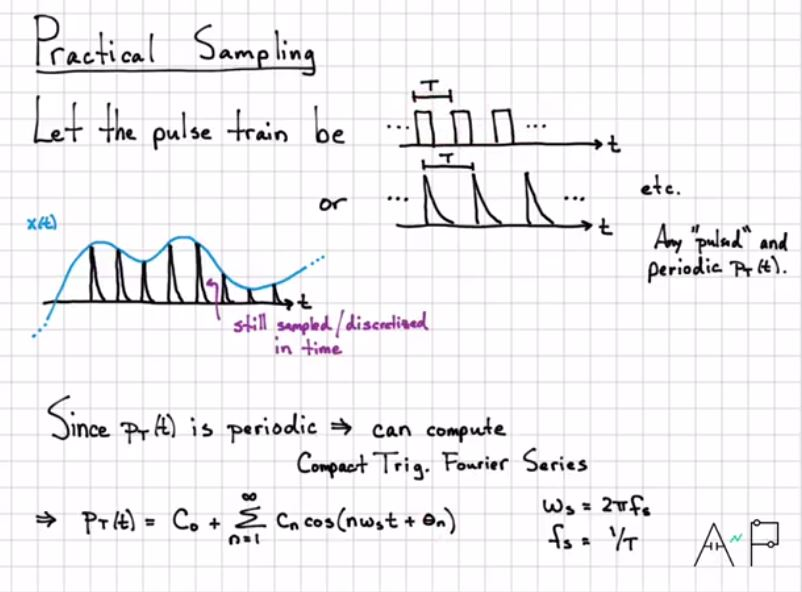
\includegraphics[width = 0.7\textwidth, frame]{Figures/Sampling/practical_sampling}
\caption{Practical Sampling using periodic finite width pulses}
\label{fig:Sampling:practical_sampling}
\end{figure}

\begin{itemize}

\item We can use any form of \tbi{periodic waveform} (square, triangular) of period $T_s$, denoted by $p_{T_s}(t)$ where $p$ stand for pulses

\item We multiply $x(t)$ by these periodic pulses, and hence we localize the signal at some discrete time interval as shown in 

\item Since the resultant of the multiplication is periodic signal, we can use the Fourier series (any form of Fourier Series, here we use the compact form)

\end{itemize}

\begin{figure}[h]
\centering
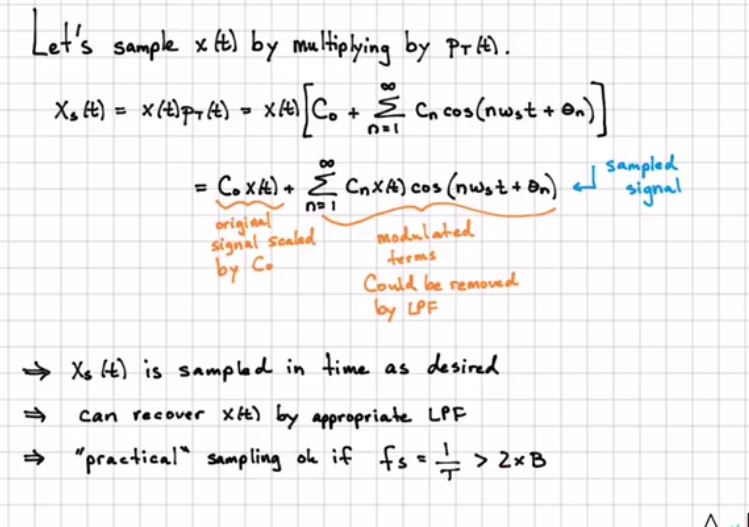
\includegraphics[width = 0.7\textwidth, frame]{Figures/Sampling/practical_sampling_2}
\caption{Practical Sampling using periodic finite width pulses: Fourier series}
\label{fig:Sampling:practical_sampling_2}
\end{figure}

\begin{itemize}

\item Notice that the signal is composed from 2 terms:

	\begin{enumerate}
	\item $C_0 \, x(t)$ which is the signal scaled by a factor $C_0$
	
	\item The modulated terms $\displaystyle\sum_{n \, = \, 1}^{+\,\infty} C_n \,\, x(t) \, \text{cos} \left( n \, \omega_s \, t \, + \, \theta_n  \right)$, which can be removed using low pass filter
	\end{enumerate}

\end{itemize}


\underline{Examples:}\\

Given are shown in \autoref{fig:Sampling:practical_sampling_example}.

\begin{figure}[h]
\centering
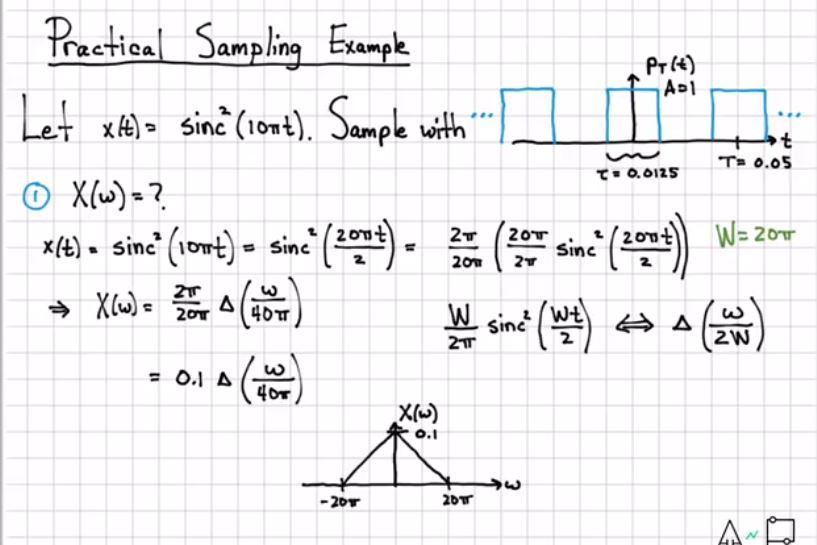
\includegraphics[width = 0.7\textwidth, frame]{Figures/Sampling/practical_sampling_example}
\caption{Practical Sampling Example}
\label{fig:Sampling:practical_sampling_example}
\end{figure}

\begin{itemize}

\item The periodic waveform we used for sampling is a square wave where the sampling period (period of the square wave) is $T_s \, = \, 0.05 $ s and pulse width $\tau \, = \, 0.0125 \, \text{s} \, = \, \displaystyle\frac{T_s}{4}$ 

\item $x(t) \, = \, \text{sinc}^2 (10 \pi t)$ has been reformulated so we can use a look up table to deduce $X(\omega)$ which is a triangular pulse of width $40 \pi$

\item Computation and development of Fourier series shown in \autoref{fig:Sampling:practical_sampling_example_compute}, \autoref{fig:Sampling:practical_sampling_example_compute_2} and \autoref{fig:Sampling:practical_sampling_example_compute_3}  


\begin{figure}[h]
\centering
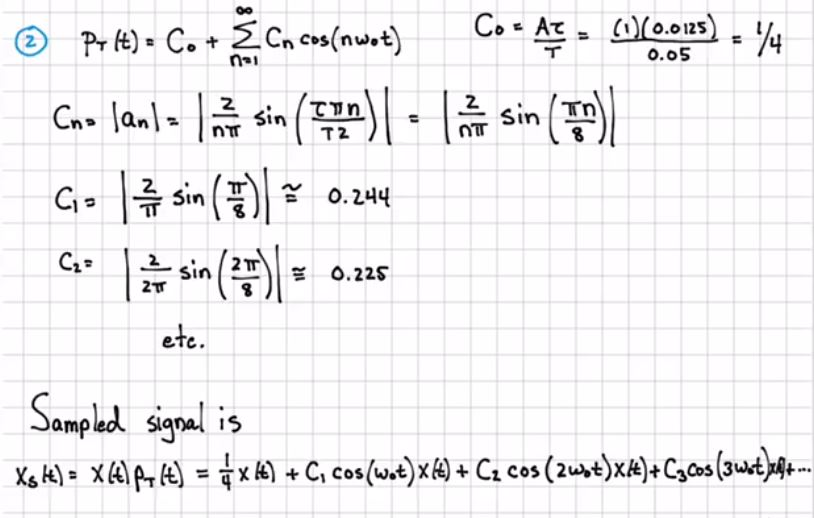
\includegraphics[width = 0.7\textwidth, frame]{Figures/Sampling/practical_sampling_example_compute}
\caption{Practical Sampling Example: Computing Fourier Series}
\label{fig:Sampling:practical_sampling_example_compute}
\end{figure}

	\begin{itemize}
	\item In \autoref{fig:Sampling:practical_sampling_example_compute}, first we develop the Fourier series of the square wave
	
	\item As a $\mathrm{2}^{nd}$ step, the sampled signal will be the product between $x(t)$ and train of square wave pulses $p_{T_s}(t)$.
	\end{itemize}

\newpage
\item Continue to expand $x_{\text{ZOH}}(t)$ (shown in \autoref{fig:Sampling:practical_sampling_example_compute_2}) where the cos is a dirac signal, and the multiplication in the time domain is a convolution in the frequency

\begin{figure}[h]
\centering
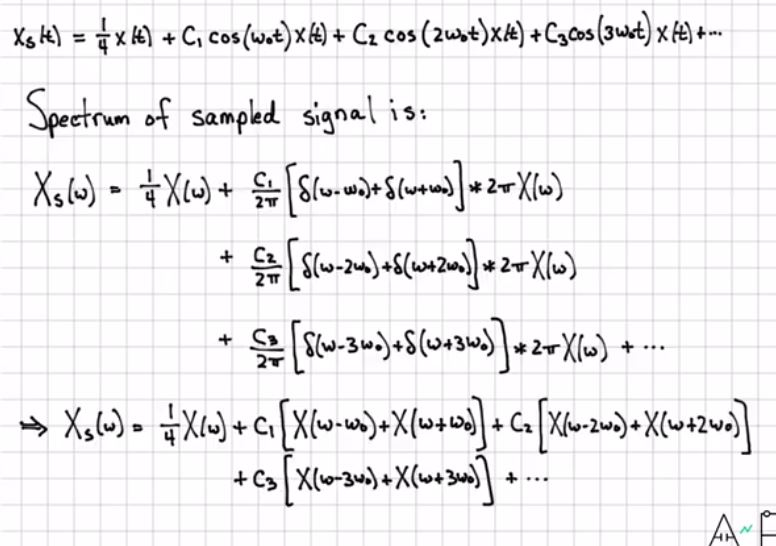
\includegraphics[width = 0.7\textwidth, frame]{Figures/Sampling/practical_sampling_example_compute_2}
\caption{Practical Sampling Example: Computing Fourier Series}
\label{fig:Sampling:practical_sampling_example_compute_2}
\end{figure}


	\begin{itemize}
	\item Then we use the convolution property of a signal with a dirac function
	\end{itemize}

\item Sketching the amplitude spectrum of $x_{\text{ZOH}}(t)$ (shown in \autoref{fig:Sampling:practical_sampling_example_compute_3})

\begin{figure}[h]
\centering
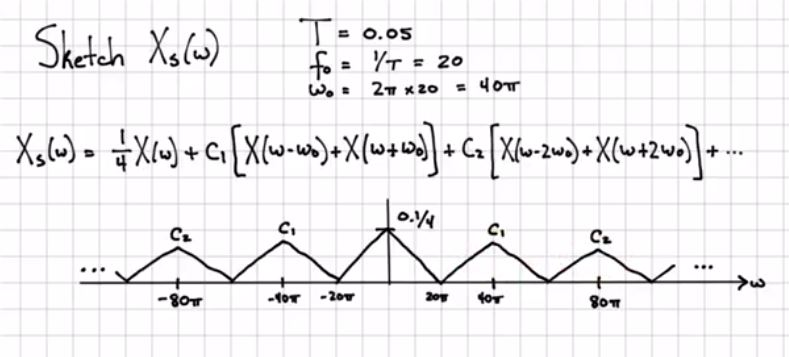
\includegraphics[width = 0.7\textwidth, frame]{Figures/Sampling/practical_sampling_example_compute_3}
\caption{Practical Sampling Example: Amplitude Spectrum of $x_{\text{ZOH}}(t)$}
\label{fig:Sampling:practical_sampling_example_compute_3}
\end{figure}

\end{itemize}




\newpage
\section{Ideal Reconstruction}

After we have seen the ideal sampling method, our goal now is to \tbi{undo the effect of sampling} and reconstruct back the continuous time signal.\\

Some people call this process \tbi{reconstruction} or \tbi{interpolation}.\\


It should be noted that the \tbi{results} developed \tbi{in this section} are \tbi{under the conditions that}:

\begin{enumerate}

\item The signal is in time is \tbi{not time limited} (so not truncation in time)

\item And its is \tbi{bandlimited}

\end{enumerate}

Practical sampling and reconstruction will be developed later in \autoref{Sec:Sampling:Practical_Sampling and_Reconstruction}.

\subsection{Sampling theorem and the Uniqueness of Reconstruction}

Suppose we have been given some set of discrete values as shown in  \autoref{fig:Sampling:example_reconstruction}.

\begin{figure}[h]
\centering
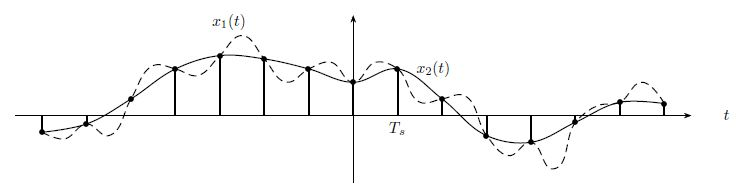
\includegraphics[width = 0.7\textwidth, frame]{Figures/Sampling/example_reconstruction}
\caption{Which signal is the correct one ?}
\label{fig:Sampling:example_reconstruction}
\end{figure}

There are many ways to plot a signal using these discrete values: one can plot and obtain $x_1(t)$ and another can obtain $x_2(t)$, so how can we ensure which signal is the correct one?\\

We can do this using the frequency representation of the sampling studied in the previous sections and using the sampling theorem, which is stated formally in \autoref{fig:Sampling:sampling_theorem_definition}.


\begin{figure}[h]
\centering
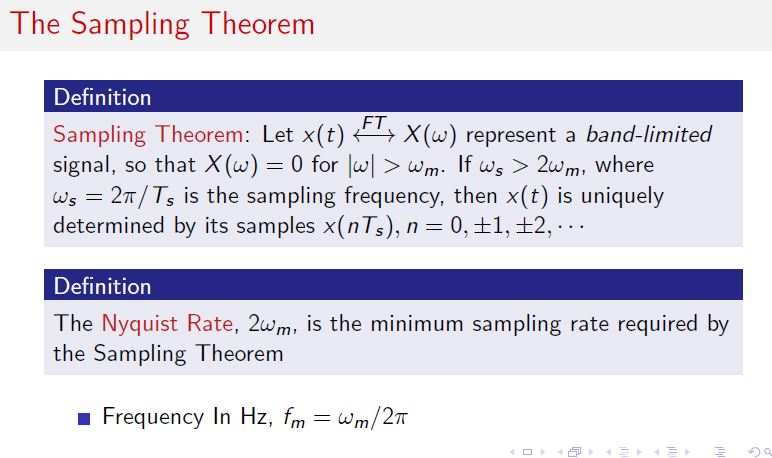
\includegraphics[width = 0.7\textwidth, frame]{Figures/Sampling/sampling_theorem_definition}
\caption{Sampling Theorem Definition}
\label{fig:Sampling:sampling_theorem_definition}
\end{figure}

\begin{itemize}

\item Notice that sampling theorem is for \tbi{band limited signal}

\item The sampling theorem give us an \tbi{upper bound} that we should sample at least from $2 \, \omega_m$ to avoid aliasing and reconstruct the signal back

\end{itemize}

\subsection{Ideal (Sinc) Interpolation}

Now we develop the mathematical model for reconstruction for impulse sampling case. Given that we have the impulse sampled spectrum as shown in \autoref{fig:Sampling:impulse_reconstruction}, how we can get back to the original spectrum ?

\begin{figure}[h]
\centering
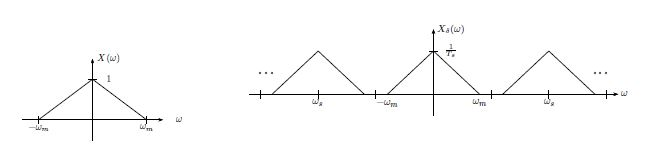
\includegraphics[width = 0.7\textwidth, frame]{Figures/Sampling/impulse_reconstruction}
\caption{Ideal Reconstruction: Spectrum of Original Signal and Impulse Sampled Signal}
\label{fig:Sampling:impulse_reconstruction}
\end{figure}

The answer is that we need to get rid off of the replicate at multiple of $\omega_s$, and then apply the proper gain for the filter because we have the scale factor $\displaystyle\frac{1}{T_s}$, and the original spectrum $X(\omega)$ has an max amplitude of 1 as shown in \autoref{fig:Sampling:impulse_reconstruction}.\\

The correspondent filter is shown in \autoref{fig:Sampling:Ideal_Reconstruction_Filter}.

\begin{figure}[h]
\centering
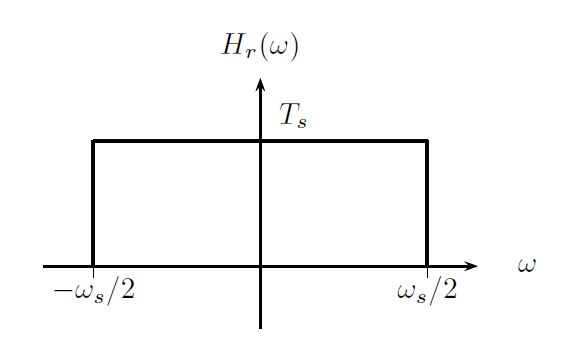
\includegraphics[width = 0.7\textwidth, frame]{Figures/Sampling/Ideal_Reconstruction_Filter}
\caption{Frequency Response of Ideal Reconstruction Filter}
\label{fig:Sampling:Ideal_Reconstruction_Filter}
\end{figure}

Now we have done the reconstruction in the frequency domain, the computations (shown in \autoref{fig:Sampling:Ideal_Reconstruction_Filter_time_domain_1} and \autoref{fig:Sampling:Ideal_Reconstruction_Filter_time_domain_2}) are also done in the time domain to understand what happens also, and how the reconstruction is done.

\begin{figure}[h]
\centering
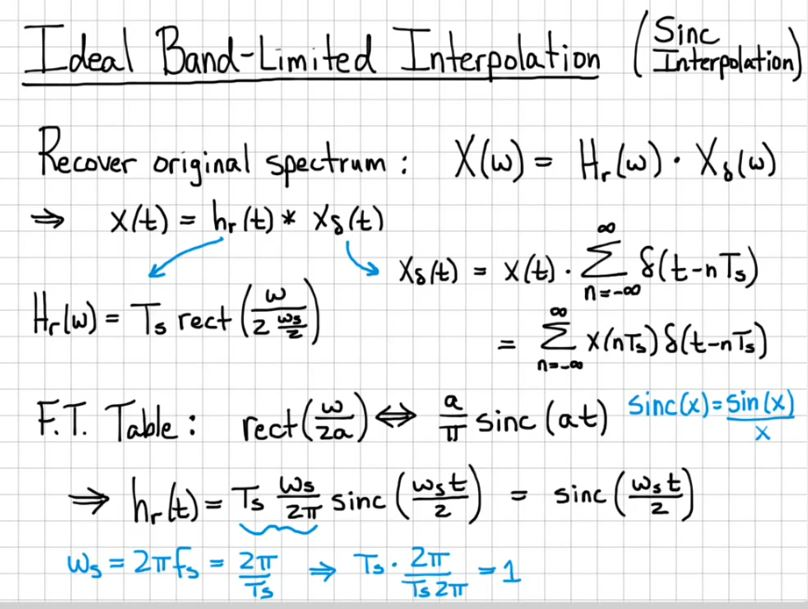
\includegraphics[width = 0.7\textwidth, frame]{Figures/Sampling/Ideal_Reconstruction_Filter_time_domain_1}
\caption{Computing $x(t)$ in the time domain starting from frequency domain formulation}
\label{fig:Sampling:Ideal_Reconstruction_Filter_time_domain_1}
\end{figure}


\begin{itemize}

\item We start from frequency domain formulation $X(\omega) \, = \, H_r(\omega) \, \times \, X_{\delta}(\omega)$


\item Multiplication in the frequency domain is convolution in the time domain

\item In $x_{\delta}(t)$, we can get $x(t)$ into the summation as $x(n \, T_s)$

\item We use some look up table to see what is $h_r(t)$.

\item Be aware to use the proper definition of $\text{sinc}(x)$

\end{itemize}


\newpage
Final form of $x(t)$ is shown in \autoref{fig:Sampling:Ideal_Reconstruction_Filter_time_domain_2}. 

\begin{figure}[h]
\centering
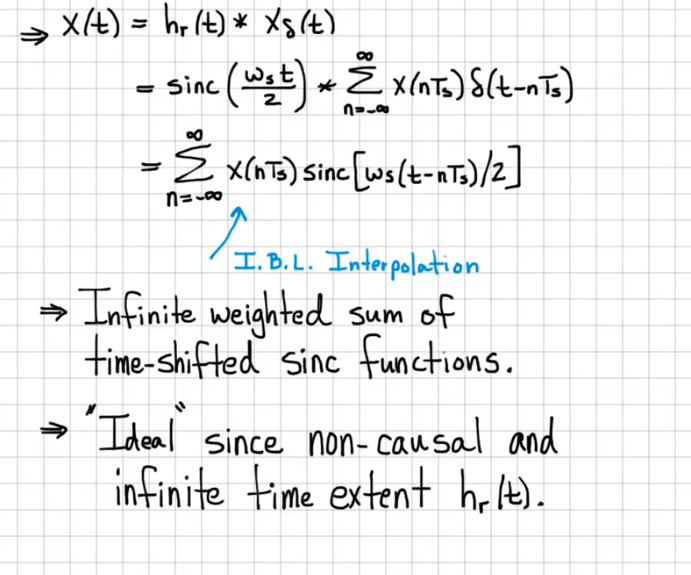
\includegraphics[width = 0.7\textwidth, frame]{Figures/Sampling/Ideal_Reconstruction_Filter_time_domain_2}
\caption{Expression of $x(t)$}
\label{fig:Sampling:Ideal_Reconstruction_Filter_time_domain_2}
\end{figure}


\begin{itemize}

\item When we multiply some signal by impulse, it will be the signal shifted to the location of the impulse

	\begin{itemize}
	\item So we get sinc into the summation and replace $t$ by $t \, - \, n\, T_s$
	
	\end{itemize}

\item So $x(t)$ is the sum of shifted sinc, each weighted by a different amplitude $x(n \, T_s)$.

\end{itemize}

\newpage
The term ideal is because the impulse response $h_r(t)$ is non causal (start before 0) and extent to infinity. A demonstration is shown in \autoref{fig:Sampling:Ideal_Reconstruction_Filter_time_domain_3}.

\begin{figure}[h]
\centering
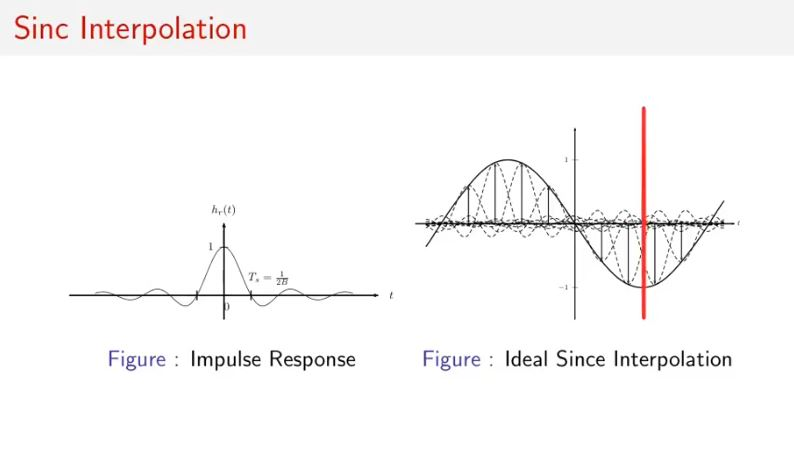
\includegraphics[width = 0.7\textwidth, frame]{Figures/Sampling/Ideal_Reconstruction_Filter_time_domain_3}
\caption{How the summation work}
\label{fig:Sampling:Ideal_Reconstruction_Filter_time_domain_3}
\end{figure}

\begin{itemize}

\item We have all these infinite sinc, and at a given time we sum all the values to obtain some value of $x(t)$.

\end{itemize}



\newpage
\section{Practical Sampling and Reconstruction}
\label{Sec:Sampling:Practical_Sampling and_Reconstruction}

Impulse sampling is one way we can get samples from the signal. Another way we can get samples is known as zero-order-hold (ZOH) as shown in \autoref{fig:Sampling:sampling_zoh}.

\begin{figure}[h]
\centering
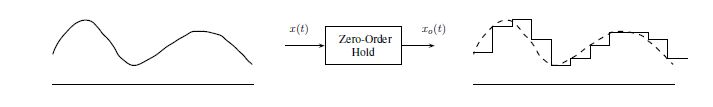
\includegraphics[width = 0.7\textwidth, frame]{Figures/Sampling/sampling_zoh}
\caption{Sampling using ZOH}
\label{fig:Sampling:sampling_zoh}
\end{figure}


It is named zero-order-hold because this filter grab a value of the signal, and then hold this value till it grab the next value. So the ZOH filter returns a stair case like signal, where each value of the signal is held till the next sampling time occurred.\\

Mathematical modeling of the ZOH is shown in \autoref{fig:Sampling:zoh_math}. 


\begin{figure}[h]
\centering
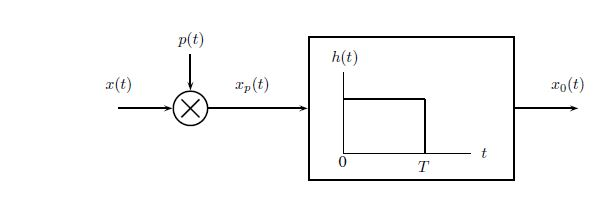
\includegraphics[width = 0.7\textwidth, frame]{Figures/Sampling/zoh_math}
\caption{Mathematical modeling of the ZOH}
\label{fig:Sampling:zoh_math}
\end{figure}


We have our continuous time signal $x(t)$ multiplied by an infinite train of pulse $p(t)$, then we obtain like before $x_p(t)$ which is equal to $x_{\delta}(t)$, then we do some low pass filtering using a pulse of width $T$. Amplitude spectrum of ZOH is shown in \autoref{fig:Sampling:zoh_amp_spectrum}. Recall that when we work in the digital domain, the only thing we care about is between $\pm \, \omega_s$.

\begin{figure}[h]
\centering
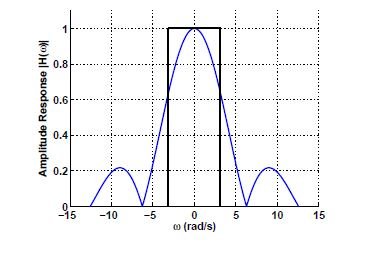
\includegraphics[width = 0.7\textwidth, frame]{Figures/Sampling/zoh_amp_spectrum}
\caption{Amplitude Spectrum of ZOH: boxed region is between $\pm \, \omega_s$}
\label{fig:Sampling:zoh_amp_spectrum}
\end{figure}


\underline{Spectrum of the Signal Compared to Impulse sampling of \autoref{fig:Sampling:impulse_sampling_spectrum_1}:}\\

Spectrum of the signal $x(t)$ using ZOH is shown in \autoref{fig:Sampling:zoh_output_spectrum}.

\begin{figure}[h]
\centering
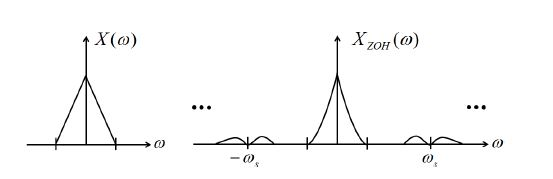
\includegraphics[width = 0.7\textwidth, frame]{Figures/Sampling/zoh_output_spectrum}
\caption{Output of ZOH in the frequency domain}
\label{fig:Sampling:zoh_output_spectrum}
\end{figure}

\begin{itemize}

\item In impulse sampling (see \autoref{fig:Sampling:impulse_sampling_spectrum_1}), the spectrum was the same (with the scale factor $\displaystyle\frac{1}{T_s}$), along with the replicate at multiple of $\omega_s$.


\item In ZOH, these replicate are attenuated due to the low pass nature of the ZOH, which is a good thing since we don't want these images.

\item However, the original spectrum is getting distorted, and this distortion is controlled by the time sampling we choose to get our values. 

\end{itemize}

\subsection{Mathematical Formulation for ZOH}

Ideal sampling followed by ideal bandlimited interpolation can't by done practically:

\begin{itemize}

\item Generating dirac pulses is very difficult

\item In reconstruction, the value of $\hat{y}(t)$ at a value of $t$ not multiple of $T_s$ is obtained by infinite sum of weighted sinc function

\item Ideal filters are also can't be made

\end{itemize}


ZOH is the practical way to grab a signal, which is done by taking a sample of the signal, and holding this value during the sampling interval.\\

Let's denote the rectangular pulse we are using by $h(t)$ denoted by:

\begin{equation}
h(t)\, = \, \begin{cases}
1 \quad 0 \, \leq \, t \, \leq \, T_s \\
0 \quad \text{otherwise}
\end{cases}
\end{equation}

The $x_{\text{zoh}}$ can be written as:

\begin{equation}
x_{\text{zoh}} \, = \, \displaystyle\sum\limits_{n \, = \, -\infty}^{\infty} x(n) h\left(	t \, - \, n\,T_s \right)
\label{Eq:Sampling:Zoh_eq_1}
\end{equation}

Recall that we can obtained a shifted version of a signal by convolving this signal with a dirac function so equation (\ref{Eq:Sampling:Zoh_eq_1}) can be further formulated:

\begin{equation}
\begin{array}{rcl}
x_{\text{zoh}} \, &=& \, \displaystyle\sum\limits_{n \, = \, -\infty}^{\infty} x(n) \, h\left(	t \, - \, n\,T_s \right) \\ \\		
&=& \, \displaystyle\sum\limits_{n \, = \, -\infty}^{\infty} x(n) \, \times \, \left[ \, \delta \left(	t \, - \, n\,T_s \right) \, * \, h(t) \, \right] \\ 
\end{array}
\label{Eq:Sampling:Zoh_eq_2}
\end{equation}


Manipulating the parenthesis of equation (\ref{Eq:Sampling:Zoh_eq_2}):

\begin{equation}
\begin{array}{rcl}
x_{\text{zoh}} \, &=& \, \displaystyle\sum\limits_{n \, = \, -\infty}^{\infty} x(n) \, h\left(	t \, - \, n\,T_s \right) \\ \\		
&=& \, \displaystyle\sum\limits_{n \, = \, -\infty}^{\infty} x(n) \, \times \, \left[ \, \delta \left(	t \, - \, n\,T_s \right) \, * \, h(t) \, \right] \\ \\
&=& \, \displaystyle\sum\limits_{n \, = \, -\infty}^{\infty} \left[\, x(n) \, \times  \, \delta \left(	t \, - \, n\,T_s \right) \, \right] \, * \, h(t)   \\ \\
&=& \,  x_{\delta}(t) \, * h(t)
\end{array}
\label{Eq:Sampling:Zoh_eq_3}
\end{equation}


Taking the Fourier transform of (\ref{Eq:Sampling:Zoh_eq_3}) we get:

\begin{equation}
\begin{array}{rcl}
X_{\text{zoh}}(\omega_c) \, &=& \, X_{\delta}(\omega_c) \, \times \, H(\omega_c) \\ \\
			 &=& \, \displaystyle\frac{1}{T_s} \, \displaystyle\sum\limits_{n  =  -\infty}^{\infty} X_a \left( \, \omega_c \, - \,  n \, \omega_s \right) \, \times \, 2 \, \text{exp}\left( \, -j \, \displaystyle\frac{\omega_c \, T_s}{2} \, \right) \, \times \, \text{sinc}\left(\, \displaystyle\frac{\omega_c \, T_s}{2} \,\right) 
\end{array}
\end{equation}

Since the rectangular pulse of \autoref{fig:Sampling:zoh_math} is not centered at 0, and it is shifted by $\displaystyle\frac{T_s}{2}$, we obtain a phase shift of $ 2 \, \text{exp}\left( \, -j \, \displaystyle\frac{\omega_c \, T_s}{2} \, \right)$ multiplying the sinc function.


\subsection{Reconstruction for ZOH}


Time delay by the factor of  $\displaystyle\frac{T_s}{2}$ can't be corrected, we have to deal with it. However, the distortion in original spectrum and the replication can be fixed.\\

\underline{Key notes in designing anti-imaging filter:}

\begin{itemize}

\item the key difficulty is in the transition band, where we need to suddenly pass to 0 in the stop band

\item This can be easily achieved if we have a high transition band, which implies that $\omega_s >> \,$ bandwidth signal

\item We later get back to this point when covering oversampling and undersampling, and how they can make the design of the anti-imaging filter less or more expensive.

\end{itemize}




\newpage
\section{Spectral Sampling}
\label{Sec:Sampling:Sepctral_Sampling}


After we have been dealing with the sampling theorem, which tells what are the minimum number of samples we need from the time domain to construct a correct waveform, we move now to the dual form, which is \tbi{sampling in the frequency domain} and derive the number of samples in the spectrum required to construct the time domain signal. We are expecting similar results due to the time-frequency duality we now from Fourier transform lessons.

Explanation shown in \autoref{fig:Sampling:sepctral_sampling_replication_time_signal}.


\begin{figure}[h]
\centering
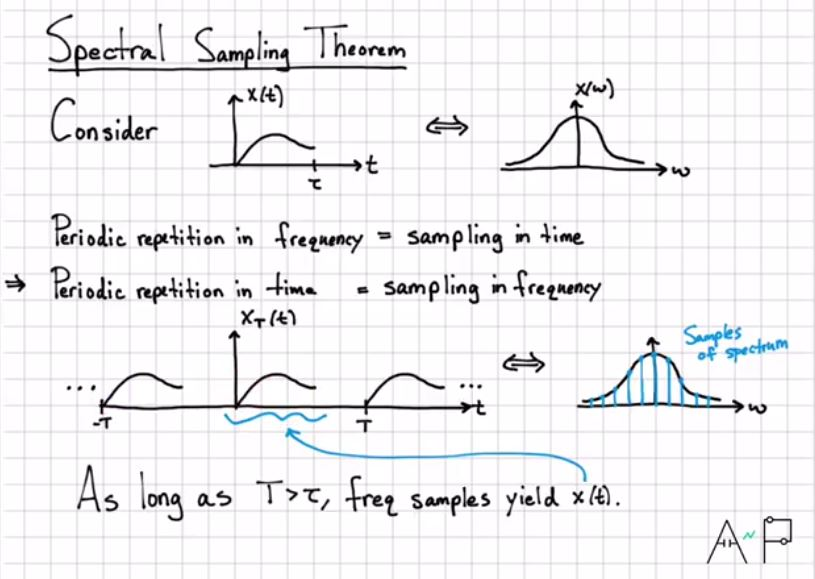
\includegraphics[width = 0.7\textwidth, frame]{Figures/Sampling/sepctral_sampling_replication_time_signal}
\caption{Replicating the time signal give us samples in the frequency domain}
\label{fig:Sampling:sepctral_sampling_replication_time_signal}
\end{figure}

\begin{itemize}

\item We are assuming we have a time limited domain signal $x(t)$ of duration $\tau$.

\item We know from \autoref{Sec:Sampling:Sampling_Continuous_Time_Signals} that sampling in time give us replication of the spectrum in the frequency domain

	\begin{itemize}
	\item The dual form now is that replicating in time give us samples in the frequency domain
	
	\item More generally, sampling in one domain give us replication in the $\mathrm{2}^{nd}$ domain
	\end{itemize}

\end{itemize}

\newpage
Now moving to deal with the mathematical development which relates the samples of $X(\omega)$ with $X(\omega)$ itself, shown in \autoref{fig:Sampling:sepctral_sampling_math_formulation}.


\begin{figure}[h]
\centering
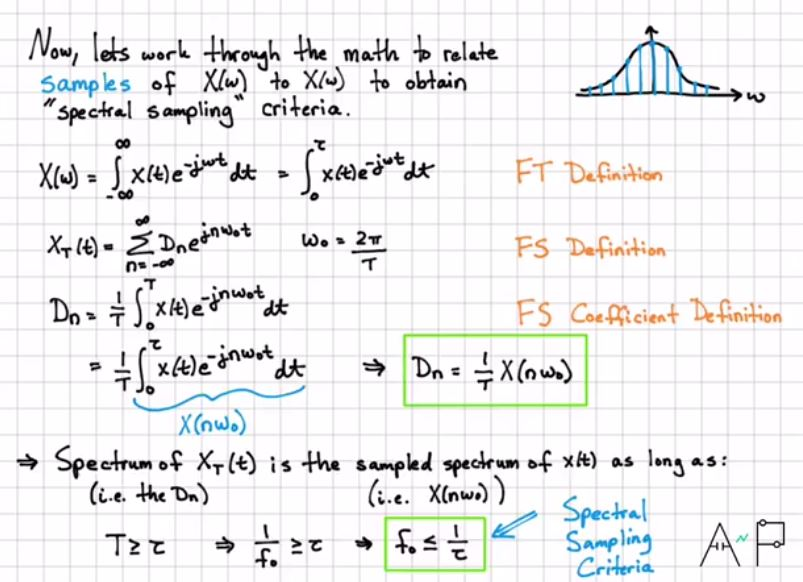
\includegraphics[width = 0.7\textwidth, frame]{Figures/Sampling/sepctral_sampling_math_formulation}
\caption{Mathematical formulation between samples of $X(\omega)$ and $X(\omega)$ itself}
\label{fig:Sampling:sepctral_sampling_math_formulation}
\end{figure}


\begin{itemize}

\item We start by Fourier transform definition

\item Since we are replicating in the time domain now, we can use Fourier series on $x_T(t)$

\item Notice the relation between $D_n$ and $X(\omega)$: they are the same except for the argument of the exponential:

	\begin{itemize}
	\item In $X(\omega)$, we have $\omega$
	
	\item In $D_n$, we have $n \, \omega_0$
	\end{itemize}

\end{itemize}

The \tbi{spectral sampling theorem} tells us: if we want to \tbi{describe a continuous time-limited signal} from its \tbi{spectrum samples}, we need to make sure that the \tbi{frequency spacing} $ \left(\, f_0 \, = \, \displaystyle\frac{1}{T} \, \right)$ is less than the inverse of the signal duration $\displaystyle\frac{1}{\tau}$







\section{Applications}


Sampling theorems let us replace a continuous time signal with a discrete set of numbers, so all we have to do now is to process these discrete numbers.\\ 

In this section we will look to some application of sampling, like how we can use the sample values to change the characteristic of a pulse.

A pulse can have different characteristics, like amplitude, width, position,$\cdots$. We start first by the following type of pulse modulation: PAM, PWM, PPM, and then treat PCM separately because it is the most sophisticated one among them.


\subsection{PAM, PWM and PPM}

\autoref{fig:Sampling:pulse_modulation} shows different type of pulse modulation

\begin{figure}[h]
\centering
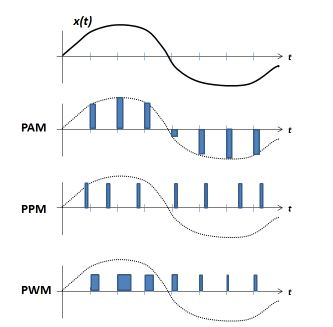
\includegraphics[width = 0.7\textwidth, frame]{Figures/Sampling/pulse_modulation}
\caption{Pulse Modulation}
\label{fig:Sampling:pulse_modulation}
\end{figure}

\begin{itemize}

\item In PAM: the more the sample value is higher, the amplitude of the pulse is higher

	\begin{itemize}
	\item The more the value is negative, same of the amplitude of the pulse
	\end{itemize}

\item In PPM, the width and amplitude of the pulses are all the same. However, the position of the pulse change

	\begin{itemize}
	\item If the value is more positive, the pulse become more early before the sample value
	
	\item If the value is negative, the pulse will be delayed and come after the sample value
	
	\item So we can now about sample value depending if the pulse arrive more early (more positive) or more delayed (more negative)
	\end{itemize}

\end{itemize}


\subsection{Quantization and A/D Process}

Before getting into PCM, we need to do learn some concepts whihc are prerequist to PCM. Let's start by some definitions:

\begin{itemize}

\item \tbi{Digital Signal:} discrete time signal and also discrete amplitude values

	\begin{itemize}
	\item Another definition of digital signal is that can be any continuous time signal which represents a stream of bits, like in PCM
\end{itemize}


\item \tbi{Quantization:} the process of rounding continuous valued amplitudes to a set of discrete amplitudes	

\begin{itemize}
\item Continuous-Time Signals Are Converted To Digital Signals By
Sampling and Quantizing (A/D converters do this)
\end{itemize} 

\item L-ary signal: A digital signal that can take on L different values

	\begin{itemize}
	\item Advantages of digital signal: resiliant to noise, use
of repeaters, error correction scheme more easy on digital signal (as opposite to continuous time signal which can take any value),
	\end{itemize}

\end{itemize}

\underline{Example of Quantization:}\\


\begin{figure}[h]
\centering
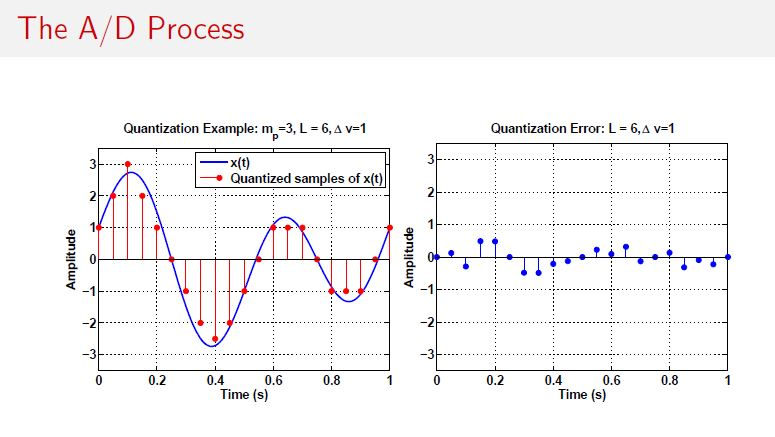
\includegraphics[width = 0.7\textwidth, frame]{Figures/Sampling/quantizaiton_example}
\caption{Quantization Example}
\label{fig:Sampling:quantizaiton_example}
\end{figure}


\begin{itemize}

\item In A/D process, first we sample the signal then we round up the value to a defined level

\item The parameters of the quantization (rounding) are:

	\begin{enumerate}
	\item The number of levels $L$: here we have 6 levels
	
	\item The step size between each level $\delta v$
	
	\item The peak value of the signal $m_p$
	\end{enumerate}


\newpage
\item Now \tbi{rounding introduce errors}, known here as \tbi{quantization error}

	\begin{itemize}
	\item If we want to decrease the quantization error, we need to increase the number of levels $L$ as \autoref{fig:Sampling:quantizaiton_example_2}
	
	\item However we need to allocate more bits to represents all of these levels (trade off)
	
	
	\begin{figure}[h]
\centering
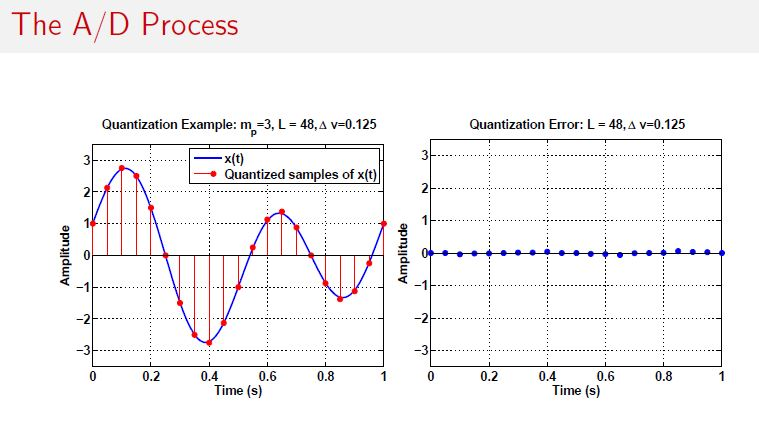
\includegraphics[width = 0.7\textwidth, frame]{Figures/Sampling/quantizaiton_example_2}
\caption{Increasing number of levels $L$ to decrease quantization error}
\label{fig:Sampling:quantizaiton_example_2}
\end{figure}
	
	\end{itemize}

\end{itemize}


\subsection{PCM}

PCM is a modulation scheme where we represent a stream of bits (after sampling and quantizing) into a sequence of pulses. An example is shown in \autoref{fig:Sampling:pcm_modulation}


\begin{figure}[h]
\centering
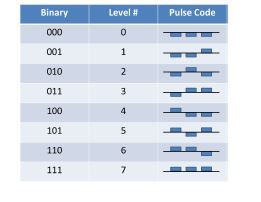
\includegraphics[width = 0.7\textwidth, frame]{Figures/Sampling/pcm_modulation}
\caption{PCM modulation using $L \, = \, 8$ levels}
\label{fig:Sampling:pcm_modulation}
\end{figure}

\begin{itemize}

\item After finishing the A/D process, we do mapping to these discrete numbers into a stream of bits


\item The the stream of bits is represented using pulses

	\begin{itemize}
	\item 1 using an positive pulse and 0 using a negative pulse
	\end{itemize}

\end{itemize}

\section{Practical Digital Filtering and Oversampling}


\begin{figure}[h]
\centering
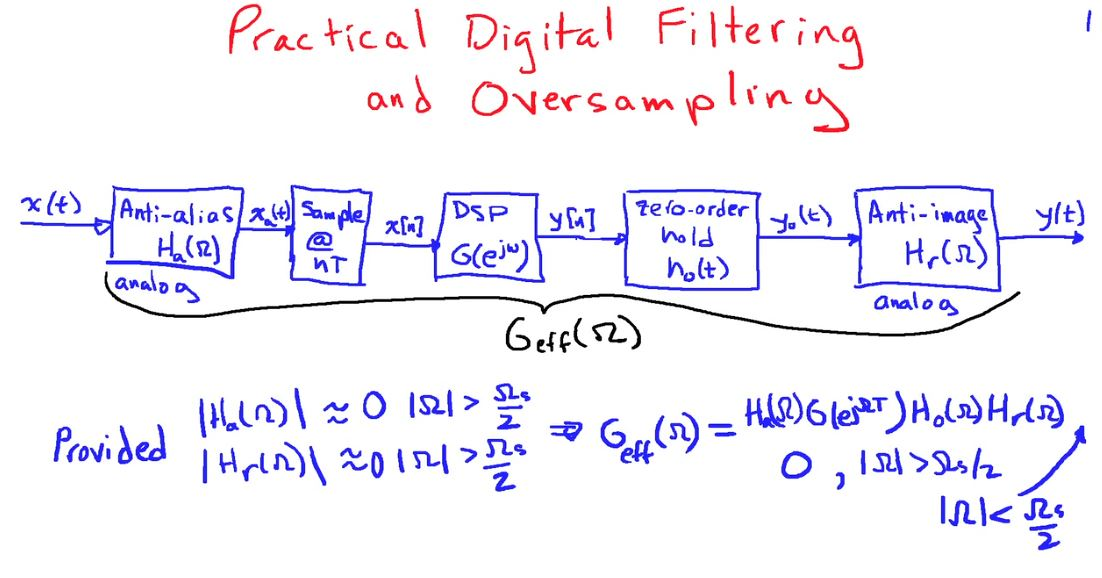
\includegraphics[width = 0.7\textwidth, frame]{Figures/Sampling/overall_sampling_reconstruction}
\caption{Overall Sampling and Reconstruction process}
\label{fig:Sampling:overall_sampling_reconstruction}
\end{figure}

\begin{itemize}

\item The DSP system is in the discrete frequency domain $\omega_d$

\end{itemize}

We can replace the whole system by a equivalent analog filter called $G_{\text{eq}}(\omega_c)$ where the transfer function is the multiplication of each transfer function block.

\subsection{Building Analog filters}


There are 2 filters presented in \autoref{fig:Sampling:overall_sampling_reconstruction} which are both \tbi{analog}: the anti-aliasing filter $H_{\text{ant}}(\omega_c)$ which cut high frequency to \tbi{prevent folding} and anti-imaging filter $H_{\text{ant-img}}(\omega_c)$ to \tbi{smooth the signal} after the ZOH operation.\\




\begin{itemize}

\item  For the anitliasing filter: if $\displaystyle\frac{\omega_s}{2}$ is close to the bandwidth of the signal $\omega_{\text{signal}}$, this means that the \tbi{transition band} of the filter is \tbi{very narrow} and that's \tbi{hard to implement in analog filters}.


\item For the anti-imaging filter: in the pass-band of the filter, we need to implement the inverse of the sinc to compensate the distortion made by the main lobe of the ZOH filter.

We need to make $\omega_s$ larger compared to the bandwidth of the signal so we don't have narrow band transition and the pass band 

\end{itemize}


So in summary, we need a high sampling rate. But in implementation, this comes at the cost excessive memory storage, because if my sampling rate is high, I have more data to process in a 1s, which means we need more memory for the storage.\\

So there is a trade-off between a high sampling rate and the memory needed for storage.

As a solution, we will change the sampling rate in the system of \autoref{fig:Sampling:overall_sampling_reconstruction}:

\begin{itemize}

\item Decrease the sampling rate after the ADC process, right before the discrete processing

\item Increase the sampling rate right before the ZOH

\end{itemize}


The new process including upsampling and downsampling is shown in \autoref{fig:Sampling:up_down_sampling}. 


\begin{figure}[h]
\centering
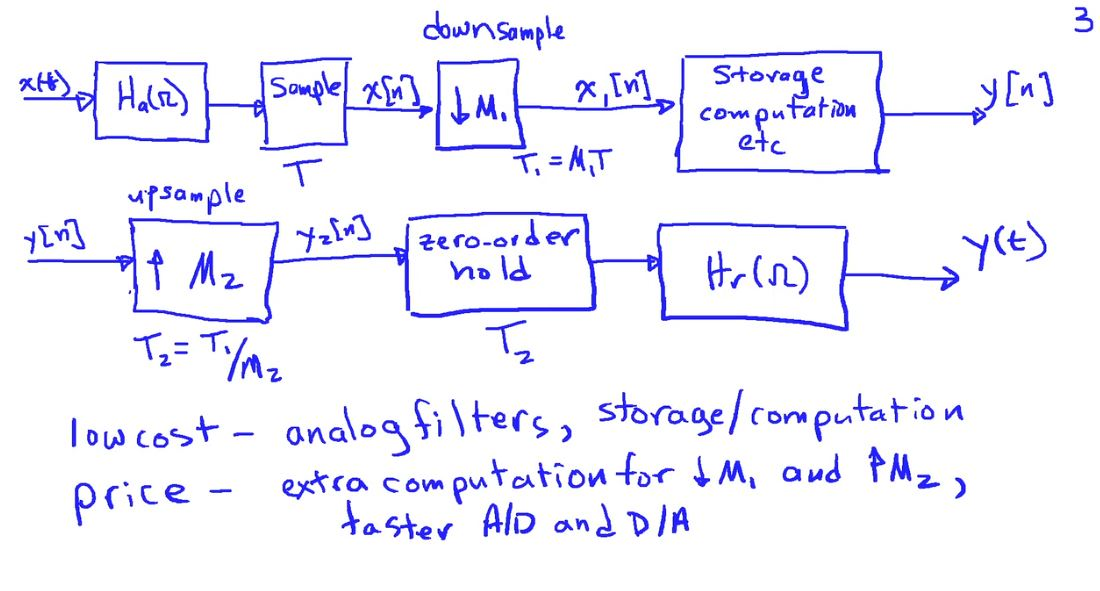
\includegraphics[width = 0.7\textwidth, frame]{Figures/Sampling/up_down_sampling}
\caption{Upsampling and downsampling for lower cost analog filters}
\label{fig:Sampling:up_down_sampling}
\end{figure}


\begin{itemize}

\item There are many efficient numerical methods to implement the up and down sampling operations

\item The price we pay in these discrete operations is worthy and make the design of the analog filters (anti-aliasing and anti-imaging) less expensive

\end{itemize}

\newpage
\subsection{Example of Oversampling}


Given are shown in \autoref{fig:Sampling:example_oversampling}.

\begin{figure}[h]
\centering
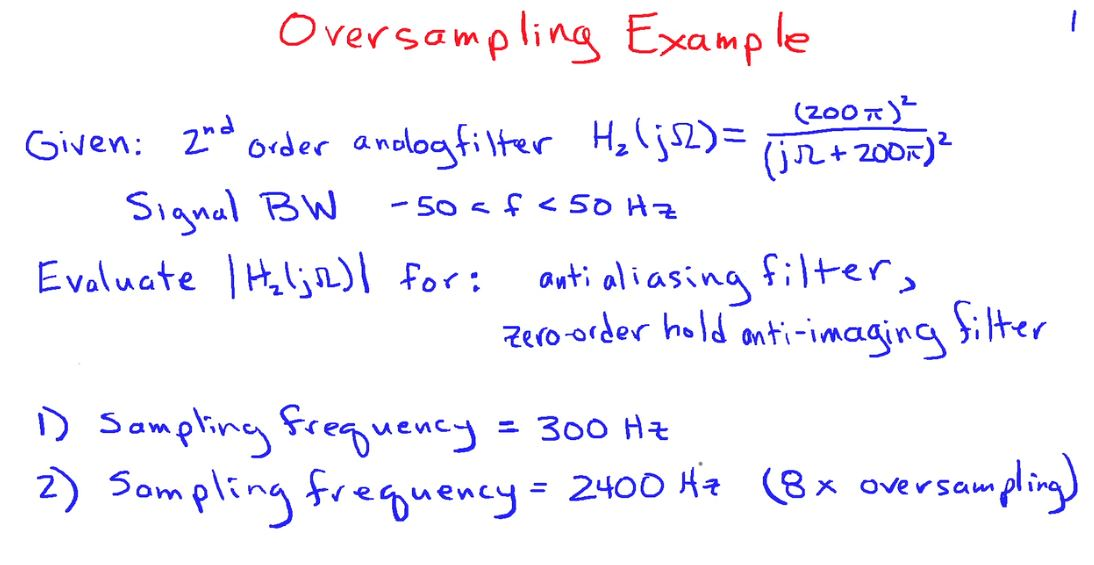
\includegraphics[width = 0.7\textwidth, frame]{Figures/Sampling/example_oversampling}
\caption{Given Example for oversampling}
\label{fig:Sampling:example_oversampling}
\end{figure}


The goal of this exercise is to show how oversampling can serve the analog filters (anti-aliasing and anti-imaging).


\begin{itemize}

\item The filter is an analog $\mathrm{2}^\mathrm{nd}$ order filter

\item The signal bandwidth is 50 Hz.

\item 2 sampling rate which both satisfy the Nyquist rate will be tested

\end{itemize}

\underline{Solution:}\\

\begin{enumerate}

\item For the anti-aliasing filter: \\

\begin{figure}[h]
\centering
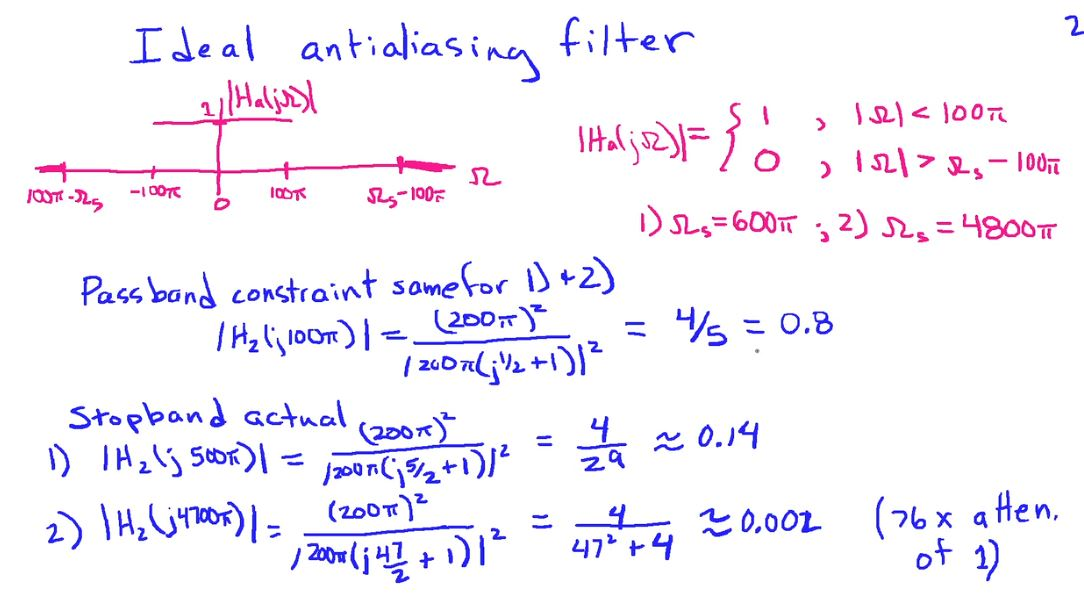
\includegraphics[width = 0.7\textwidth, frame]{Figures/Sampling/example_oversampling_sol_1}
\caption{Anti-aliasing filter solution}
\label{fig:Sampling:example_oversampling_sol_1}
\end{figure}

	\begin{itemize}
	
	\item The ideal anti-aliasing filter has an amplitude response of 1 in the pass-band and 0 in the stop band.
	
	\item Then we plug the computation for both $\omega_s$ and see the results	
	
	\begin{itemize}
	\item in the pass-band, the filtering is independent from $\omega_s$ so for both sampling rate, we have $ \mid H_{\text{ant-alias}}(\omega_c) \mid \, = \, 0.8$
	
	\item In the stop band we have the difference because the stop-band depend on $\omega_s$
	
	\end{itemize}
	
	\end{itemize}


 \item For the anti-imaging filter:

\begin{figure}[h]
\centering
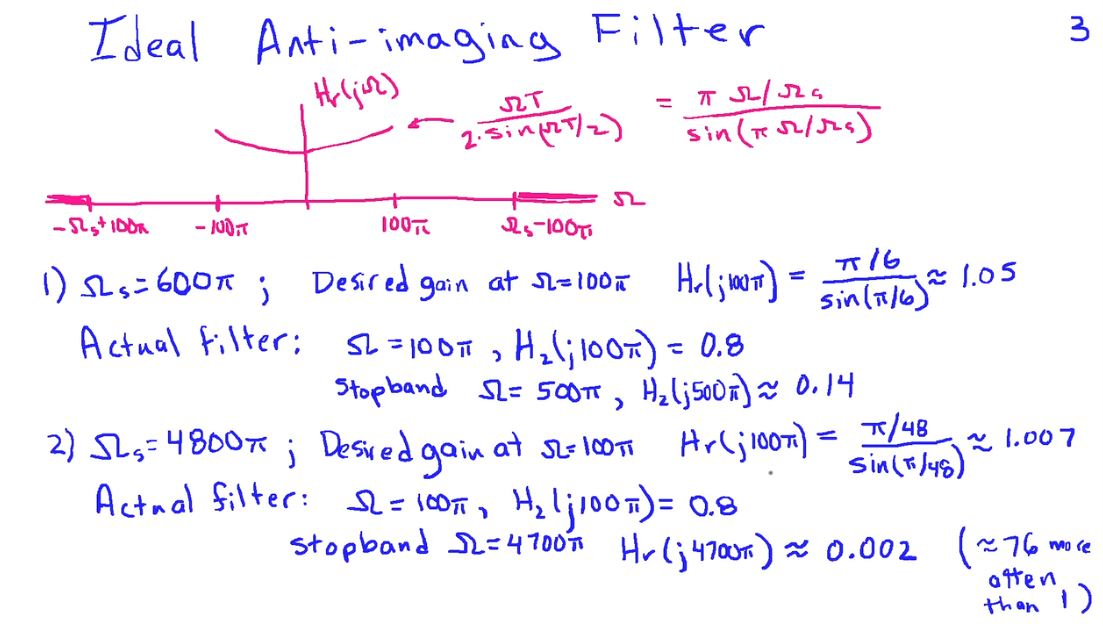
\includegraphics[width = 0.7\textwidth, frame]{Figures/Sampling/example_oversampling_sol_anti_imaging}
\caption{Anti-imaging filter solution}
\label{fig:Sampling:example_oversampling_sol_anti_imaging}
\end{figure}

\begin{itemize}

\item The ideal anti-imaging filter has the inverse of the sinc function as a frequency response


\item Also, the benefit is in the stop band, where oversampling is giving us more attenuation then the $ F_s \, = \,300 $ Hz

\end{itemize}

\end{enumerate}

\newpage
\subsection{Oversampling in D/A}

\autoref{fig:Sampling:oversampling_benefits} shows the D/A process.

\begin{figure}[h]
\centering
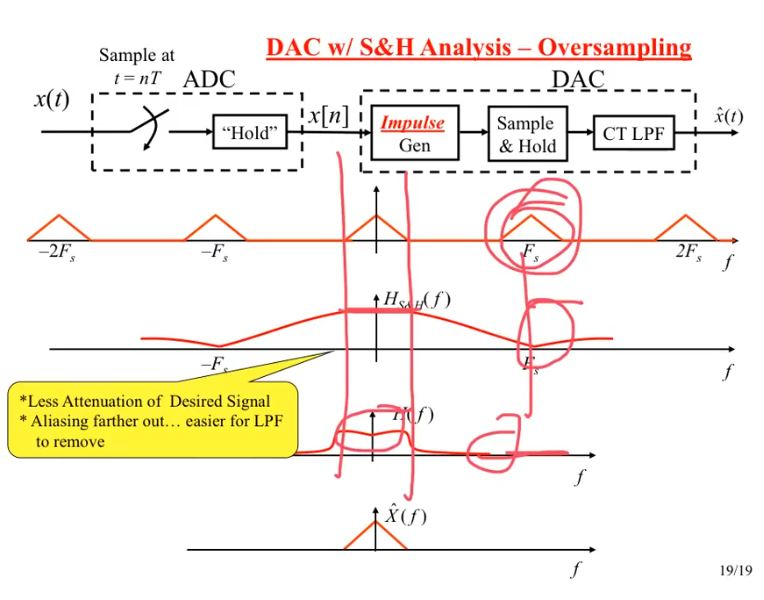
\includegraphics[width = 0.7\textwidth, frame]{Figures/Sampling/oversampling_benefits}
\caption{Over sampling Benefits}
\label{fig:Sampling:oversampling_benefits}
\end{figure}

Oversampling have several benefits:

\begin{itemize}

\item Make the frequency response of the ZOH system more flat in the pass band

\item Easier transition band design for the smoothing filter

\end{itemize}


\newpage

\section{Quantization and A/D Process}

In this section, we study quantization and its error.

\underline{Reminder:}\\

\begin{itemize}

\item \tbi{Digital Signal:} discrete time signal and also discrete amplitude values

	\begin{itemize}
	\item Another definition of digital signal is that can be any continuous time signal which represents a stream of bits, like in PCM
\end{itemize}


\item \tbi{Quantization:} the process of rounding continuous valued amplitudes to a set of discrete amplitudes	

\begin{itemize}
\item Continuous-Time Signals Are Converted To Digital Signals By
Sampling and Quantizing (A/D converters do this)
\end{itemize} 

\item L-ary signal: A digital signal that can take on L different values

	\begin{itemize}
	\item Advantages of digital signal: resiliant to noise, use
of repeaters, error correction scheme more easy on digital signal (as opposite to continuous time signal which can take any value),
	\end{itemize}

\end{itemize}

\underline{Example of Quantization:}\\


\begin{figure}[h]
\centering
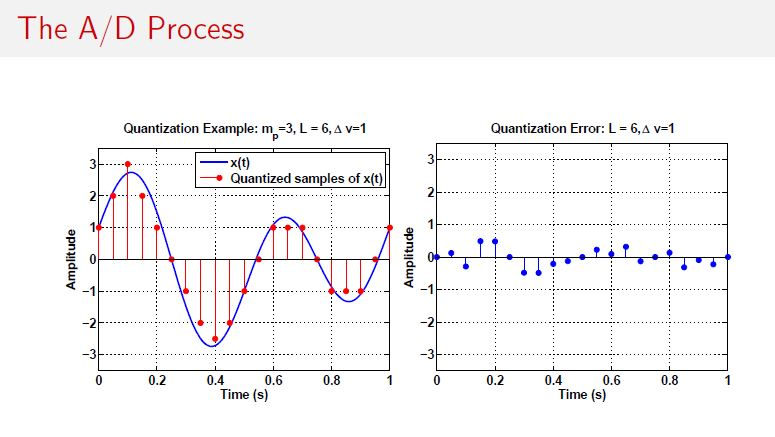
\includegraphics[width = 0.7\textwidth, frame]{Figures/Sampling/quantizaiton_example}
\caption{Quantization Example}
\label{fig:Sampling:quantizaiton_example}
\end{figure}


\begin{itemize}

\item In A/D process, first we sample the signal then we round up the value to a defined level

\item The parameters of the quantization (rounding) are:

	\begin{enumerate}
	\item The number of levels $L$: here we have 6 levels
	
	\item The step size between each level $\delta v$
	
	\item The peak value of the signal $m_p$
	\end{enumerate}


\newpage
\item Now \tbi{rounding introduce errors}, known here as \tbi{quantization error}

	\begin{itemize}
	\item If we want to decrease the quantization error, we need to increase the number of levels $L$ as \autoref{fig:Sampling:quantizaiton_example_2}
	
	\item However we need to allocate more bits to represents all of these levels (trade off)
	
	
	\begin{figure}[h]
\centering
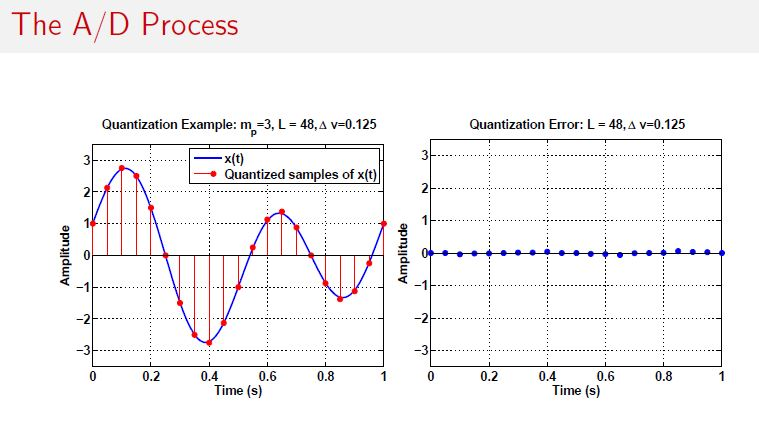
\includegraphics[width = 0.7\textwidth, frame]{Figures/Sampling/quantizaiton_example_2}
\caption{Increasing number of levels $L$ to decrease quantization error}
\label{fig:Sampling:quantizaiton_example_2}
\end{figure}
	
	\end{itemize}

\end{itemize}


\underline{Qunatization Formula:}

\begin{equation}
x_{\text{qunatized}} \, = \, \text{round} \left(\, \displaystyle\frac{x}{\text{step size}}\, \right) \, \times \, \text{step size}
\end{equation}


\newpage
\subsection{Dynamic Range of an Ideal ADC}

\begin{figure}[h]
\centering
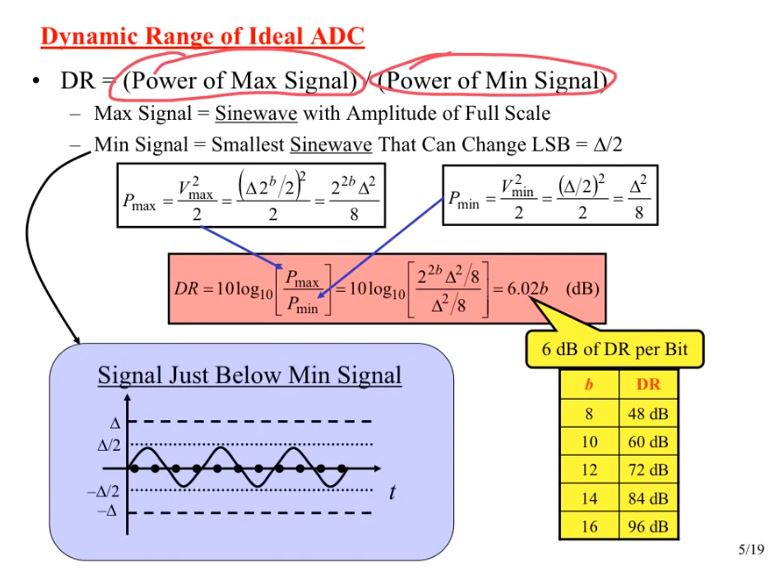
\includegraphics[width = 0.7\textwidth, frame]{Figures/Sampling/dynamic_range_ideal_adc}
\caption{Dynamic Range of an Ideal ADC}
\label{fig:Sampling:dynamic_range_ideal_adc}
\end{figure}


\subsection{Error Analysis of the Quantization Error}

Since qunantization error is unpredictable, we use statistical analysis and probability laws to describe the error.


\begin{equation}
\begin{array}{rcl}
e_q[k] \, &=& \, x[k] \, - \, x_q[k] \\\\
\displaystyle\frac{- \text{step}}{2} &\leq \, e_q[k] \, &\leq \, \displaystyle\frac{+ \text{step}}{2} \\ \\
\text{step} \, &=& \, \displaystyle\frac{\text{Range}}{\text{nb of Levels}} \\ \\
&=& \, \displaystyle\frac{\text{Range}}{2^{\left(\,\text{nb of bits + 1} \, \right)}  }
\end{array}
\end{equation}


\newpage
Error Analysis is shown in \autoref{fig:Sampling:quantizaiton_error_analysis}.

\begin{figure}[h]
\centering
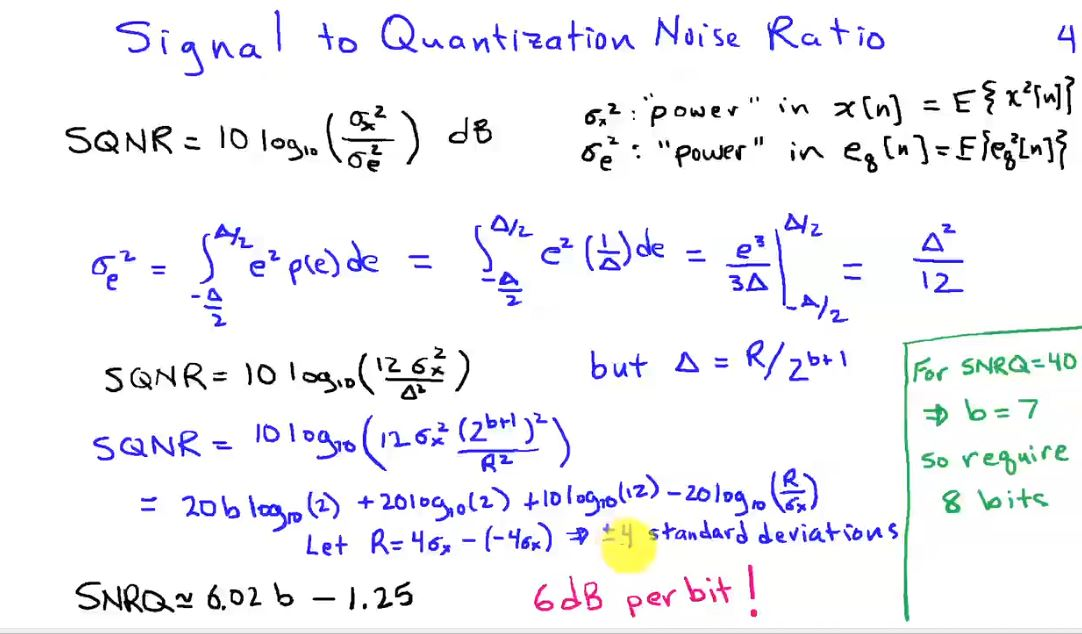
\includegraphics[width = 0.7\textwidth, frame]{Figures/Sampling/quantizaiton_error_analysis}
\caption{Qunatization Error Analysis}
\label{fig:Sampling:quantizaiton_error_analysis}
\end{figure}

\begin{itemize}

\item 

\begin{equation}
\begin{array}{rcl}
\text{SNQR} 	\, &=& \, 10 \, \text{log}_{10} \left(\, \displaystyle\frac{\sigma_x^2}{\sigma_e^2} \, \right) \\ \\
			& \approx & \, 6.02 \, - \, 1.25 \text{ dB/bit}		
\end{array}
\end{equation}


\item The analysis done is under particular assumptions for this statistical analysis:

	\begin{enumerate}
	\item $e_q[k]$ is a stationary random process with a uniform continuous distribution 
	
	\item $e_q[k]$ values are uncorrelated
	
	\item $e_q[k]$ and $x[k]$ are independent 
	\end{enumerate}

\end{itemize}


\newpage
In \autoref{fig:Sampling:quantizaiton_error_example}, we have an example of quantized and non-quantized sin.



\begin{figure}[h]
\centering
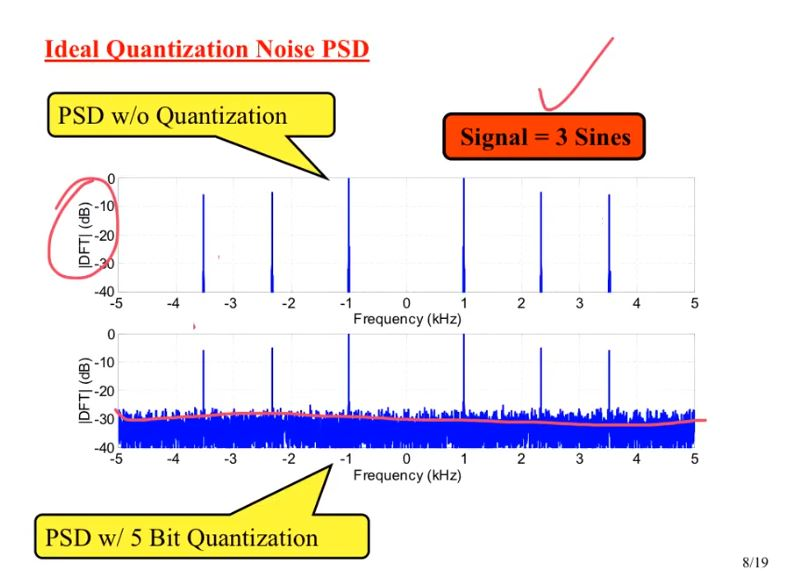
\includegraphics[width = 0.7\textwidth, frame]{Figures/Sampling/quantizaiton_error_example}
\caption{Qunatization Error Example}
\label{fig:Sampling:quantizaiton_error_example}
\end{figure}


\begin{itemize}

\item We can see that the power sepctral density in the quantized part is flat over all the frequency ranges


\item If we use fewer bit in the quantization process, the noise floor will get up

\end{itemize}


\newpage
\underline{SNQR for Full Scale Sine wave:}\\

\begin{figure}[h]
\centering
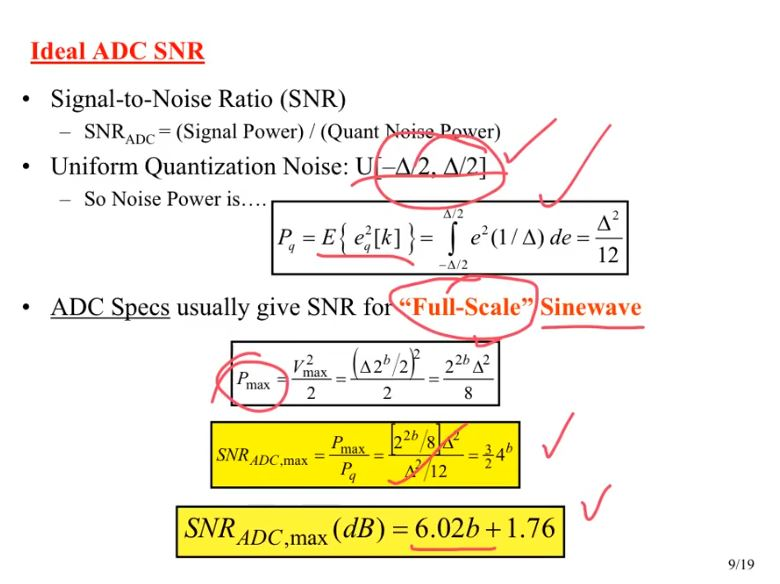
\includegraphics[width = 0.7\textwidth, frame]{Figures/Sampling/snr_full_sin_wave}
\caption{SNR for full sin wave}
\label{fig:Sampling:snr_full_sin_wave}
\end{figure}


\begin{itemize}
\item The SNQR in \autoref{fig:Sampling:snr_full_sin_wave} is a little bit optimistic because we are assuming a full range for the sin wave
\end{itemize}

We can generalize more the SNQR as in \autoref{fig:Sampling:snr_peak_factor}, where use the idea of peak factor to see the exact SNQR.


\newpage
\begin{figure}[h]
\centering
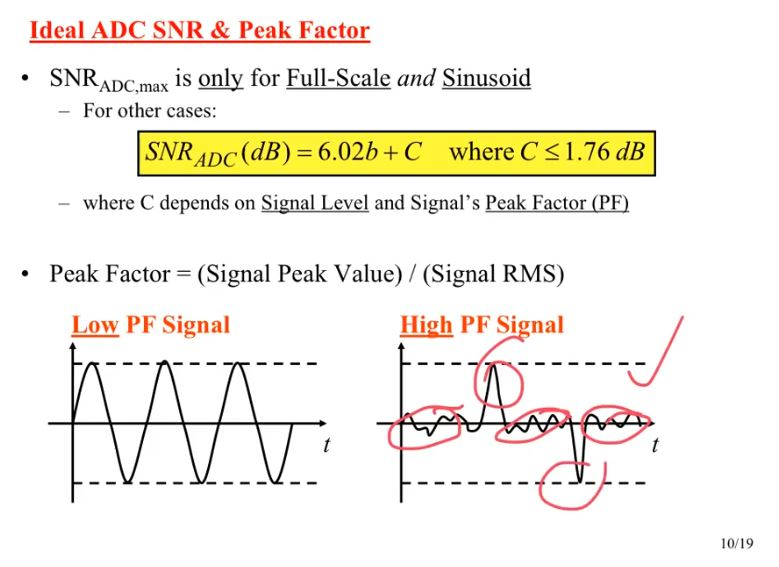
\includegraphics[width = 0.7\textwidth, frame]{Figures/Sampling/snr_peak_factor}
\caption{SNR and peak factor}
\label{fig:Sampling:snr_peak_factor}
\end{figure}

\autoref{fig:Sampling:snr_peak_factor_relation} shows the relation of SNQR and peak factor in dB.


\begin{figure}[h]
\centering
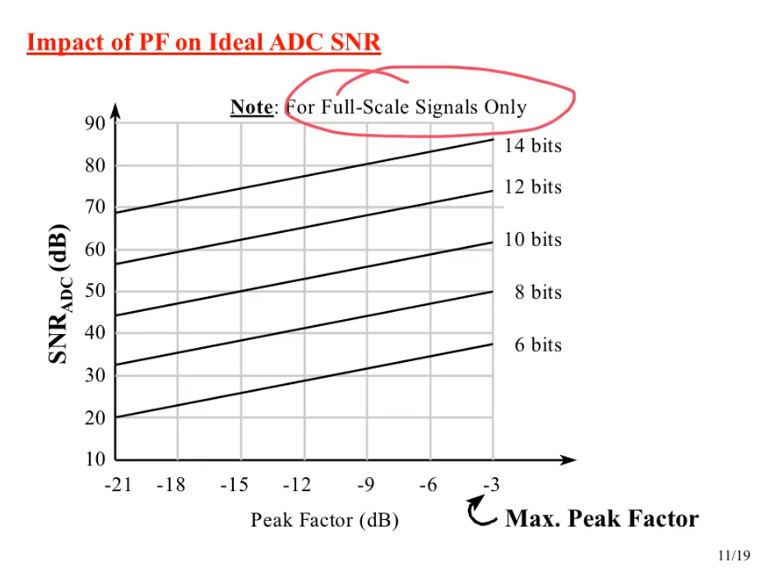
\includegraphics[width = 0.7\textwidth, frame]{Figures/Sampling/snr_peak_factor_relation}
\caption{SNR and peak factor relation}
\label{fig:Sampling:snr_peak_factor_relation}
\end{figure}

\begin{itemize}
\item The more the signal is peaky for a fixed number of bits, the more SNQR is low
\end{itemize}


\subsection{More Source of Errors}

\autoref{fig:Sampling:more_error} shows more sources of errors we can get

\begin{figure}[h]
\centering
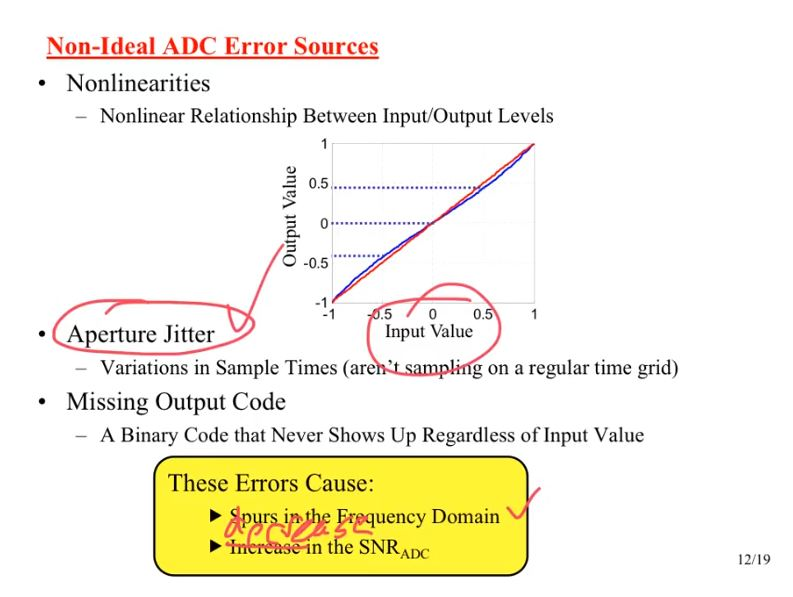
\includegraphics[width = 0.7\textwidth, frame]{Figures/Sampling/more_error}
\caption{SNR and peak factor relation}
\label{fig:Sampling:more_error}
\end{figure}

\begin{itemize}

\item Jitter: comes from clock circuitry we use to do the sampling


\item These errors also shows decrease in the SNQR

\end{itemize}

\autoref{fig:Sampling:spurse} shows how the spruse comes into the amplitude spectrum plots in addition to the noise floor.

\begin{figure}[h]
\centering
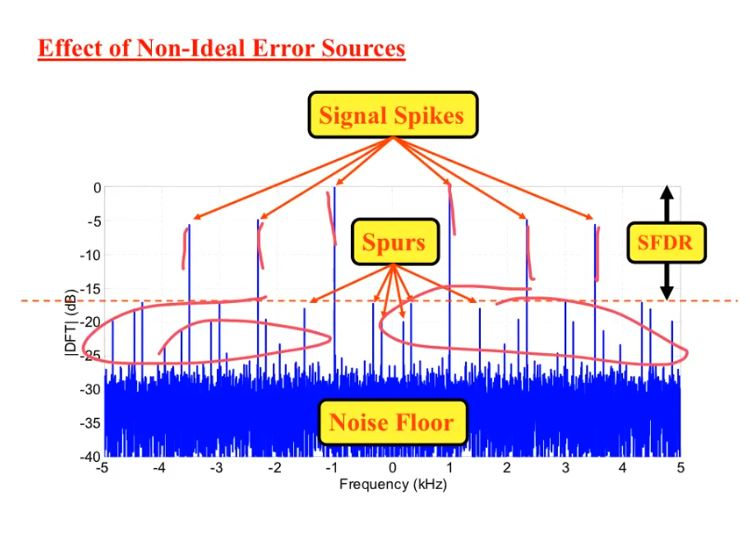
\includegraphics[width = 0.7\textwidth, frame]{Figures/Sampling/spurse}
\caption{Spurse Errors in the Spectrum}
\label{fig:Sampling:spurse}
\end{figure}

\begin{itemize}
\item SFDR set the distance between the actual signals and the spurse
\end{itemize}


\subsection{Specs for ADC}

\begin{figure}[h]
\centering
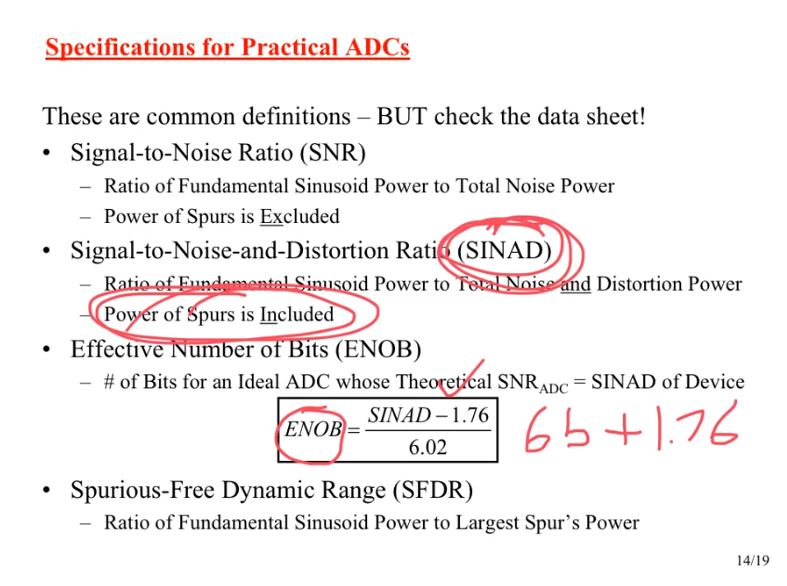
\includegraphics[width = 0.7\textwidth, frame]{Figures/Sampling/ADC_Specs}
\caption{Most common specfication on ADC}
\label{fig:Sampling:ADC_Specs}
\end{figure}

\begin{itemize}

\item ENOB: take into consideration the actual number of bits due SINAD (spurse errors)

	\begin{itemize}
	\item It is the algebraic solution of $\text{SINAD} \, = \, 6 \, \text{bits} \, + \, 1.76$
	
	\item Due to hardware imperfections (spurse), in theory we could have 8 bits, but in reality it may comes down in to 6 bits
	\end{itemize}

\end{itemize}



\newpage
\section{Oversampling and $\Sigma-\Delta$ Converter}

We have seen that oversampling have several advantages. Now let's relate the oversampling to the SNQR.



\begin{itemize}

\item Since we are sampling much higher than the signal bandwidth, we can assume that the signal bandwidth is small compared to $\displaystyle\frac{F_s}{2}$, and the spectrum reside in a small region of the interval $\left[\, \displaystyle\frac{- F_s}{2} \, ; \, \displaystyle\frac{+ F_s}{2} \right] $


\item So we have less noise in the signal spectrum $\rightarrow$ SNQR improve


\item So also ENOB improves

	\begin{itemize}
	\item However at the cost of a higher $F_s$
	\end{itemize}

\item But this is an inefficient trade-off: because we obtain 1 bit per 6 dB

	\begin{itemize}
	\item Computation shown in \autoref{fig:Sampling:oversampling_SNQR_relation}
	
	\begin{figure}[h]
\centering
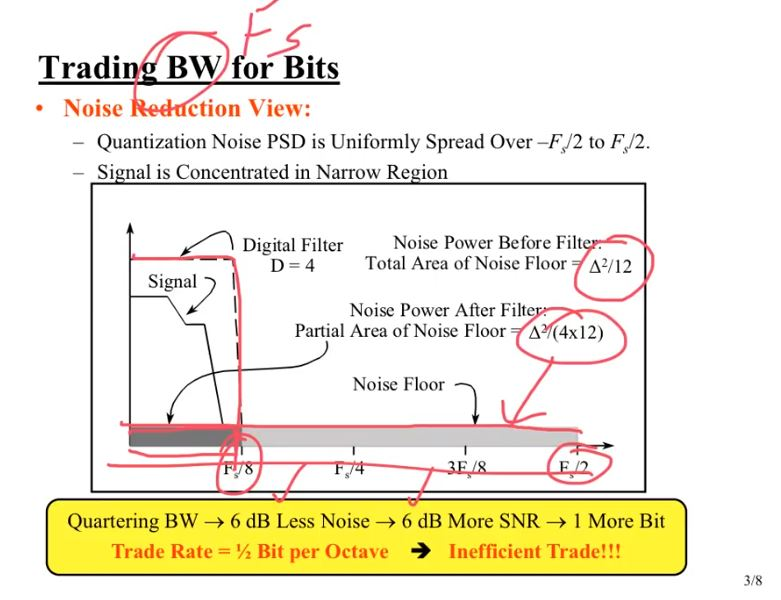
\includegraphics[width = 0.7\textwidth, frame]{Figures/Sampling/oversampling_SNQR_relation}
\caption{Oversampling and SNQR relation}
\label{fig:Sampling:oversampling_SNQR_relation}
\end{figure}	

	\item The noise power is the area under the curve then we divide powers
	
	\end{itemize}

\item So engineers start to search for a better trade-off

\item The idea of $\Sigma-\Delta$ converter: don't touch the signal but push the noise outside the signal spectrum

\newpage
\item Intuition and results are shown in \autoref{fig:Sampling:sigma_delta_noise_shaping}.

	\begin{figure}[h]
\centering
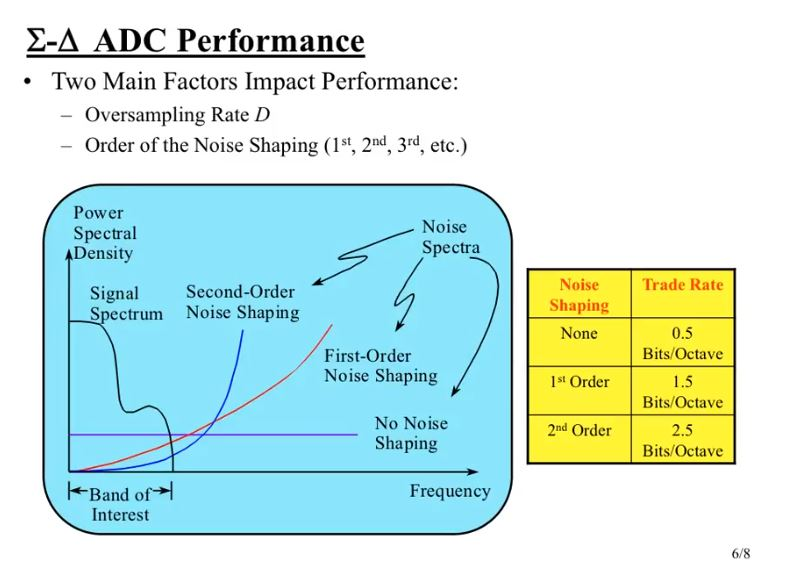
\includegraphics[width = 0.7\textwidth, frame]{Figures/Sampling/sigma_delta_noise_shaping}
\caption{Noise shaping effect}
\label{fig:Sampling:sigma_delta_noise_shaping}
\end{figure}	

	\begin{itemize}
	\item The more we increase the order of noise shaping, the area of the noise decrease and hence SNQR and ENOB increase for the \tbi{band of interest}
	\end{itemize}


\end{itemize}




\chapter{Bandpass Sampling}

Now we move to what we call bandpass sampling or higher order sampling. Before getting directly into the process, we talk first about bandpass signals in general, and how to represent them.

\begin{itemize}

\item Bandpass signal are encountered in RF application (communication and radar )


\item The amplitude spectrum is centered at a center frequency $f_c$

\item When a receiver process a transmitted signal, they don't process it in the bandpass form, they turn into what we call \tbi{equivalent low pass signal}, which is a \tbi{generalization of the idea of phasor}.

\end{itemize}

There are 3 ways of sampling in bandpass cases:

\begin{enumerate}
    \item Integer band positioning
    
    \item Non Integer Band positioning
    
    \item Quadrature sampling, which use IQ representation of a signal
    
\end{enumerate}


\section{Integer Band Positioning}

\todo{Integer Band Positioning}

\textit{To write it later}


\section{Non-Integer Band Positioning}

\todo{Non- Integer Band Positioning}

\textit{To write it later}


\newpage
\section{Quadrature Sampling}

Before, we review the concept of IQ representation.

\subsection{Review of Phasor Notation}

\underline{Phasor Idea:}\\

\begin{figure}[h]
\centering
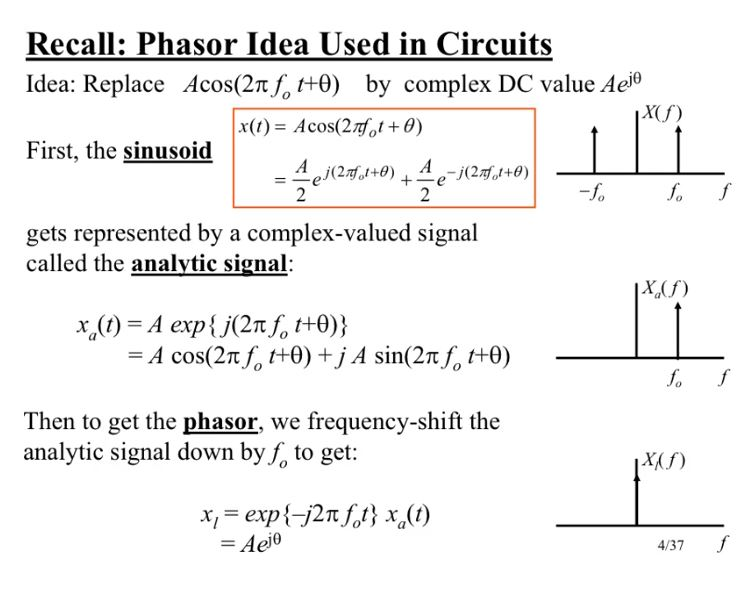
\includegraphics[width = 0.7\textwidth, frame]{Figures/Sampling/bandpass_to_lowpass_cosine}
\caption{Equivalent Low pass signal to a cosine signal}
\label{fig:Sampling:bandpass_to_lowpass_cosine}
\end{figure}

\begin{itemize}

\item We have some bandpass signal $x(t) \, = \, A \, \text{cos}\left(\, 2 \pi f_0 \, + \, \theta  \,\right)$

\item Using Euler formula, we obtain 2 dirac function at $f_0$ and $- f_0$

\item Turn the signal into analytically form by suppressing the negative frequency component at $-f_0$

\item Then we shift the component at $+f_0$ to dc by multiplying by $\text{exp}\left(\, -j 2 \pi f_0 t \,\right)$

	\begin{itemize}
	\item The obtained signal is called $x_{low-pass}$ which is \tbi{complex value signal}
	\end{itemize}

\end{itemize}


\newpage
\subsection{Equivalent Low Pass Signal}

We can generalize this idea into a general bandpass signal, as shown in \autoref{fig:Sampling:bandpass_to_lowpass_general}.


\begin{figure}[h]
\centering
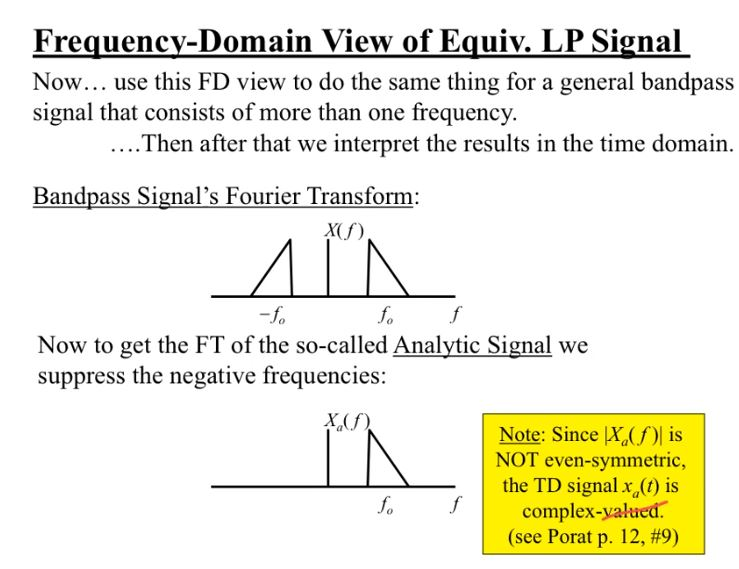
\includegraphics[width = 0.7\textwidth, frame]{Figures/Sampling/bandpass_to_lowpass_general}
\caption{Equivalent Low pass signal to a general bandpass signal}
\label{fig:Sampling:bandpass_to_lowpass_general}
\end{figure}


\begin{itemize}

\item Be aware that since $X_{\text{analyticall}}(f_c)$ has no symmetry around the y-axis, this means that $x_{\text{analyticall}}(t)$ is \tbi{complex signal}

\end{itemize}

\newpage
So we start by a real value bandpass signal, and turn it into a complex value low pass signal.  \\

A system point of view for implementing the suppression of the negative frequency part is shown in \autoref{fig:Sampling:hilbert_bandpass_lowpass}, where $H(f_c)$ is known as Hilbert transform.

\begin{figure}[h]
\centering
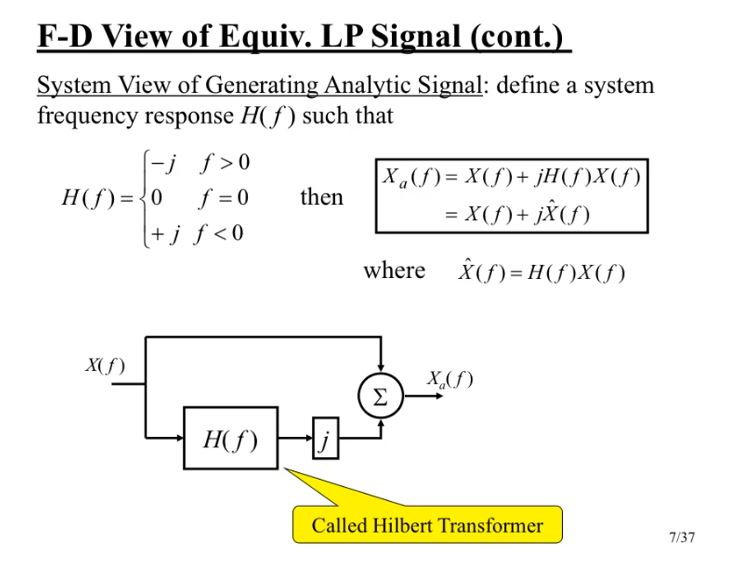
\includegraphics[width = 0.7\textwidth, frame]{Figures/Sampling/hilbert_bandpass_lowpass}
\caption{System point of view to implement the suppression of negative frequency spectrum}
\label{fig:Sampling:hilbert_bandpass_lowpass}
\end{figure}


\begin{itemize}

\item We apply Hilbert transform to $X_{\text{band-pass}}(f_c)$, then add the output with the original signal $X_{\text{band-pass}}(f_c)$

\end{itemize}

\newpage
After we obtain $X_{\text{analyticall}}(f_c)$ which is a complex signal, we shift down the frequency spectrum and hence we obtain $X_{\text{low-pass}}(f_c)$  as shown in \autoref{fig:Sampling:shift_frequency_down}. 

\begin{figure}[h]
\centering
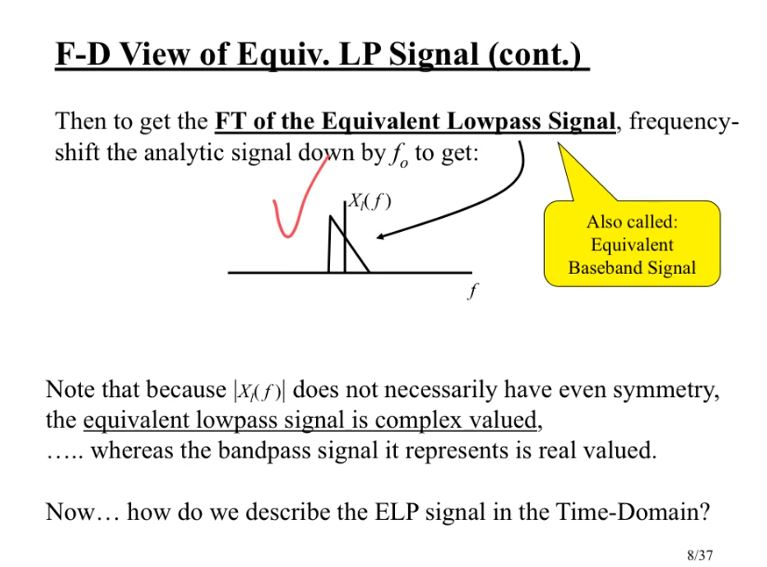
\includegraphics[width = 0.7\textwidth, frame]{Figures/Sampling/shift_frequency_down}
\caption{Shifting down the frequency spectrum of $X_{\text{analyticall}}(f_c)$}
\label{fig:Sampling:shift_frequency_down}
\end{figure}


\subsection{Recap}

So as a recap of the process in terms of formulas:

\begin{enumerate}

\item We begin from a general band-pass signal $x_{\text{band-pass}}(t)$

\item Obtain its analytic form:

\begin{equation}
\begin{array}{rcl}
X_{\text{analytic}}(f_c) \, &=& \, X_{\text{band-pass}}(f_c) \, + \, j \, X_{\text{Hilber}}(f_c) \\ \\
x_{\text{analytic}}(t) \, &=& \, x_{\text{band-pass}}(t) \, + \, j \, x_{\text{Hilber}}(t) \\ \\
\end{array}
\end{equation}

\item Down frequency shifting to obtain $x_{\text{Eq-Baseband}}(t) \in \mathbb{C}$:

\begin{equation}
\begin{array}{rcl}
x_{\text{Eq-Baseband}}(t) \, &=& \, \text{exp}\left(\, -j 2 \pi f_{\text{center}} \, t \,\right) \, \times \, x_{\text{analytic}}(t) \\ \\
	&=& \, \text{exp}\left(\, -j 2 \pi f_{\text{center}} \, t \,\right) \, \times \, \left[\,  x_{\text{band-pass}}(t) \, + \, j \, x_{\text{Hilber}}(t) \,\right]
\end{array}
\end{equation}

\item Since  $x_{\text{Eq-Baseband}}(t)$ is a \tbi{complex signal}, we can \tbi{express it in a rectangular form} known also as in-phase and quadrature form

\begin{equation}
\begin{array}{rcl}
x_{\text{Eq-Baseband}}(t) \, &=& \, \text{exp}\left(\, -j 2 \pi f_{\text{center}} \, t \,\right) \, \times \, x_{\text{analytic}}(t) \\ \\
	&=& \, \text{exp}\left(\, -j 2 \pi f_{\text{center}} \, t \,\right) \, \times \, \left[\,  x_{\text{band-pass}}(t) \, + \, j \, x_{\text{Hilber}}(t) \,\right] \\ \\
	&=& \, x_{\text{in-phase}}(t) \, + \, j \, x_{\text{quadrature}}(t)
\end{array}
\end{equation}

\item  The purpose know is to find the relation between $x_{\text{band-pass}}(t)$ and in-phase and quadrature of $x_{\text{Eq-Baseband}}(t)$.

\begin{equation}
\begin{array}{rcl}
x_{\text{band-pass}}(t) \, &=& \, x_{\text{in-phase}}(t) \, \text{cos}\left(\, 2 \pi \, f_{\text{center}} \, t \,\right) + \, x_{\text{quadrature}}(t) \, \text{sin}\left(\, 2 \pi \, f_{\text{center}} \, t \,\right) \\ \\

\text{Similarly but less important} \\ 
x_{\text{Hilber}}(t) \, &=& \, x_{\text{in-phase}}(t) \, \text{sin}\left(\, 2 \pi \, f_{\text{center}} \, t \,\right) + \, x_{\text{quadrature}}(t) \, \text{cos}\left(\, 2 \pi \, f_{\text{center}} \, t \,\right) 
\end{array}
\end{equation}


\item Final form using polar form between bandpass signal and equivalent baseband signal

\begin{equation}
\begin{array}{rcl}
x_{\text{band-pass}}(t) \, &=&\, \text{Amp}(t) \, \times \, \text{cos}\left(\, 2 \pi \, f_{\text{center}} \, t \, + \, \text{phase}(t) \,\right)\\ \\
\end{array}
\label{Eq:Sampling:based_band_general_form_time_domain}
\end{equation}

where $\begin{cases}
x_{\text{Eq-Baseband}}(t) \, = \, \text{Amp}(t)\,\times \, \text{exp}\left[\, j \,\times \, \text{phase}(t) \,\right] \\ \\
\text{Amp}(t) \, = \, \sqrt{ x_{\text{in-phase}}^2(t) \, + \, x_{\text{quadrature}}^2(t)} \\ \\
\text{phase}(t) \,  = \, \text{tan}^{-1}\left[\, \displaystyle\frac{x_{\text{in-phase}}(t)}{x_{\text{quadrature}}(t)} \,\right] 
\end{cases}$

	\begin{itemize}
	
	\item The equivalent baseband signal $x_{\text{Eq-Baseband}}(t)$ has the same envelope and phase of the original bandpass signal $x_{\text{band-pass}}(t)$ 	
	
	\item The conditions for equation (\ref{Eq:Sampling:based_band_general_form_time_domain}) is that the amplitude and the phase vary slowly compared to carrier signal. \\
	
	If not, equation (\ref{Eq:Sampling:based_band_general_form_time_domain}) won't be bandpass signal in necessarily.
	\end{itemize}

\end{enumerate}

\section{Generation of I and Q components}




As a recap, we have:

\begin{equation}
\begin{array}{rcl}
x_{\text{band-pass}}(t) \, &=&\, \text{Amp}(t) \, \times \, \text{cos}\left(\, 2 \pi \, f_{\text{center}} \, t \, + \, \text{phase}(t) \,\right)\\ \\
\end{array}
\label{Eq:Sampling:based_band_general_form_time_domain_recap}
\end{equation}


In communication and radar signal processing, we usually process the I and Q components of the bandpass signal where:

\begin{equation}
\begin{array}{rcl}
x_{\text{in-phase}}(t) \, &=& \, \text{Amp}(t) \, \times \, \text{cos}\left[\, \text{phase}(t) \, \right] \\ \\
x_{\text{quadrature}}(t) \, &=& \, \text{Amp}(t) \, \times \, \text{sin}\left[\, \text{phase}(t) \, \right] \\ \\
\end{array}
\label{Eq:Sampling:inpahse_quadrature_signals}
\end{equation}

\newpage
To implement these signals of equation (\ref{Eq:Sampling:inpahse_quadrature_signals}), we begin first from manipulating equation using trigonometric identities as shown in \autoref{fig:Sampling:IQ_trigonometric_identities}, then building these signals using analog devices as shown in \autoref{fig:Sampling:qudrature_impelmentation}.


\begin{figure}[h]
\centering
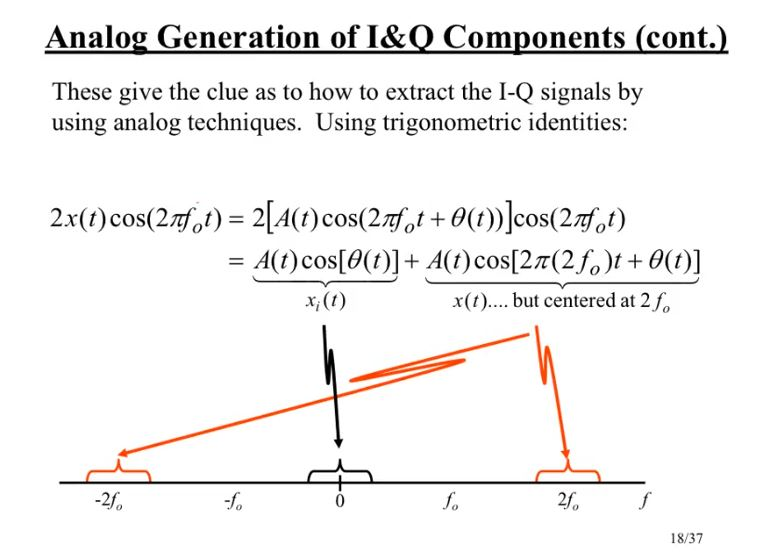
\includegraphics[width = 0.7\textwidth, frame]{Figures/Sampling/IQ_trigonometric_identities}
\caption{Inphase term generation }
\label{fig:Sampling:IQ_trigonometric_identities}
\end{figure}

\begin{itemize}

\item We use the trigonometric identities of the argument of a cos

\item Notice that we obtained the in-phase term, but with a high frequency component centered at $2\, f_{\text{ceneter}}$, so we need to use a low pass filter

\end{itemize}


\begin{figure}[h]
\centering
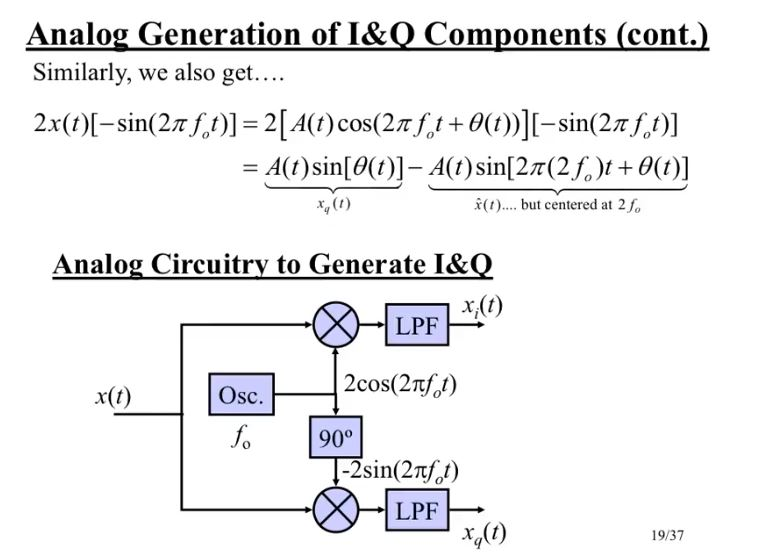
\includegraphics[width = 0.7\textwidth, frame]{Figures/Sampling/qudrature_impelmentation}
\caption{IQ generation and implementation using analog devices}
\label{fig:Sampling:qudrature_impelmentation}
\end{figure}

\begin{itemize}

\item The multiplication is a mixer and the phase shift is implemented using a phase shifter

\item The cos signal is generated using an oscillator

\end{itemize}

Also, the in-phase and quadarature components can be generated digitally, as shown in, using some DSP processor.

\begin{itemize}

\item Instead of a mixer, we can do multiplication numerically

\item Instead of an oscillator, we can do generate the cos numerically also

\end{itemize}


\section{Sampling Dilemma using I and Q Components}

Suppose we have generate the I and Q components and we want to process them in a system for some purpose. Usually, we put some ADC after the I and Q to do the processing in discrete time.\\

According to Shannon theorem, we need to sample twice as fast the highest frequency component, which is $B$ according to , if we take the $X_{\text{Eq-Baseband}}(f_c)$ amplitude spectrum.\\

However, the original band pass signal $X_{\text{Bandpas}}(f_c)$ has a bandwidth of $B$, so according to Shannon, we need to sample at $2 \, B$.

\begin{figure}[h]
\centering
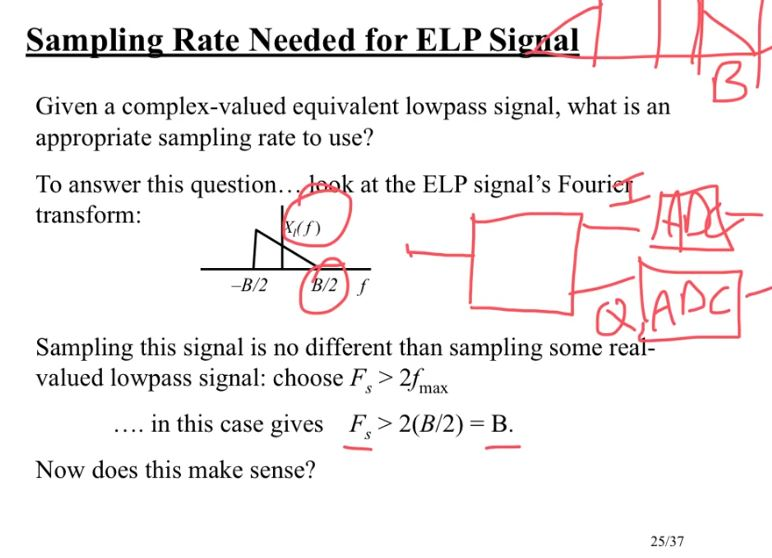
\includegraphics[width = 0.7\textwidth, frame]{Figures/Sampling/sampling_IQ}
\caption{IQ sampling}
\label{fig:Sampling:sampling_IQ}
\end{figure}

\newpage
But we need not to forget that $X_{\text{Eq-Baseband}}(f_c)$ is composed from 2 signals, and each signal is sampled at a rate of $B$, which make sense.

\begin{figure}[h]
\centering
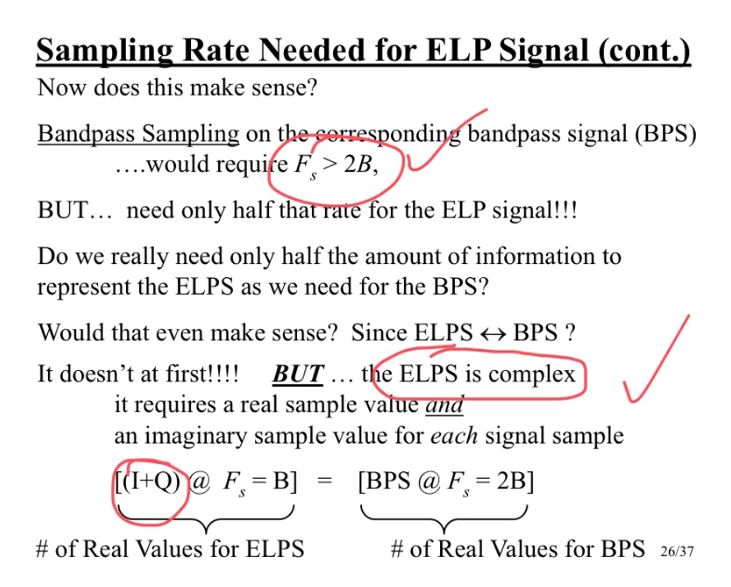
\includegraphics[width = 0.7\textwidth, frame]{Figures/Sampling/sampling_IQ_2}
\caption{IQ sampling: each component is sampled at a rate of $B$}
\label{fig:Sampling:sampling_IQ_2}
\end{figure}


\newpage
\subsection{Integer band positioning}


\begin{figure}[h]
\centering
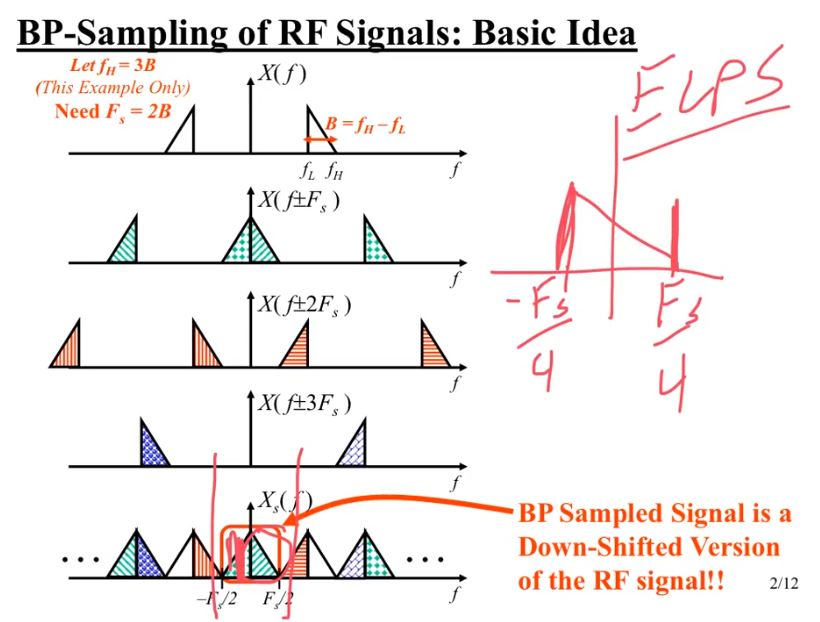
\includegraphics[width = 0.7\textwidth, frame]{Figures/Sampling/bandpass_sampling_ex_1}
\caption{Bandpass sampling example 1}
\label{fig:Sampling:bandpass_sampling_ex_1}
\end{figure}

\begin{itemize}

\item We have a bandpass signal of bandwidth $B$ and $f_{\text{high}} \, = \, 3B$

\item The theory tells us that we need to sample at twice the maximum frequency in the signal, so $F_s \, = \, 6B$


\item However, in the example of \autoref{fig:Sampling:bandpass_sampling_ex_1}, we sample at $F_s \, = \, 2B$


\item When we sample $F_s \, = \, 2B$, the theory tells to add the replicate of the spectrum at multiple of $F_s$

	\begin{itemize}
	\item Each portion of the spectrum (positive and negative) will be shifted at multiple of $F_s$
	\end{itemize}


\item At the end we obtain $X_{\text{sampled}}(f_c)$

	\begin{itemize}

	\item To reconstruct the bandpass signal, we low pass the signal then shifted to obtain the equivalent base band signal
	
	
	\end{itemize}



\end{itemize}


\newpage
\underline{General Case:}\\


\begin{figure}[h]
\centering
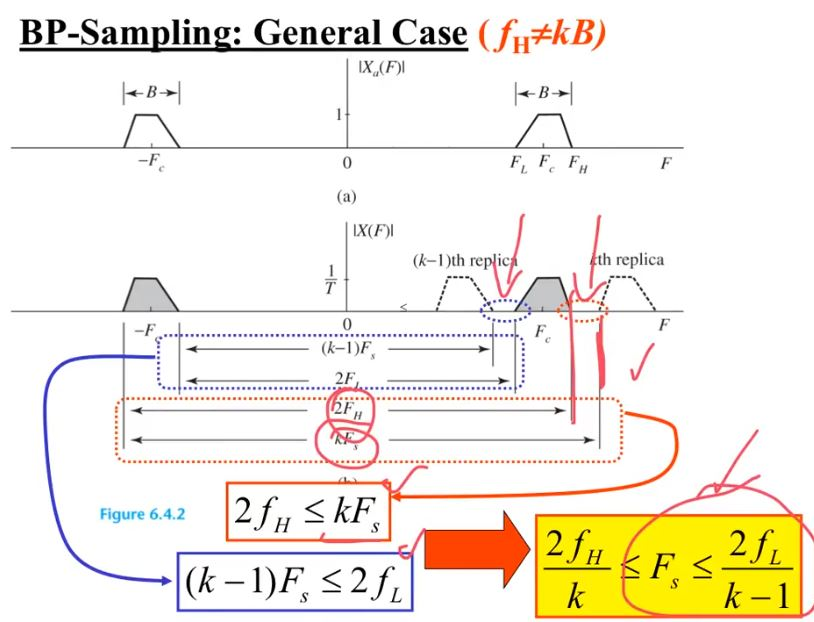
\includegraphics[width = 0.7\textwidth, frame]{Figures/Sampling/bandpass_sampling_general_case_non_integer}
\caption{Bandpass sampling non integer case}
\label{fig:Sampling:bandpass_sampling_general_case_non_integer}
\end{figure}

\begin{itemize}

\item We want that the images don't overlap with the original spectrum of the bandpass signal

\item The 2 inequality contstraints comes from $f_{\text{low}}$ and $f_{\text{high}}$

\item The larger $k$ we have, the lower $F_s$ we can choose.

	\begin{itemize}
	\item However, we don't have an idea about $k$ yet
	\end{itemize}

\newpage
\item Now we formulate a bound on $k$ shown in \autoref{fig:Sampling:bandpass_sampling_general_case_non_integer_bound_k}.


\begin{figure}[h]
\centering
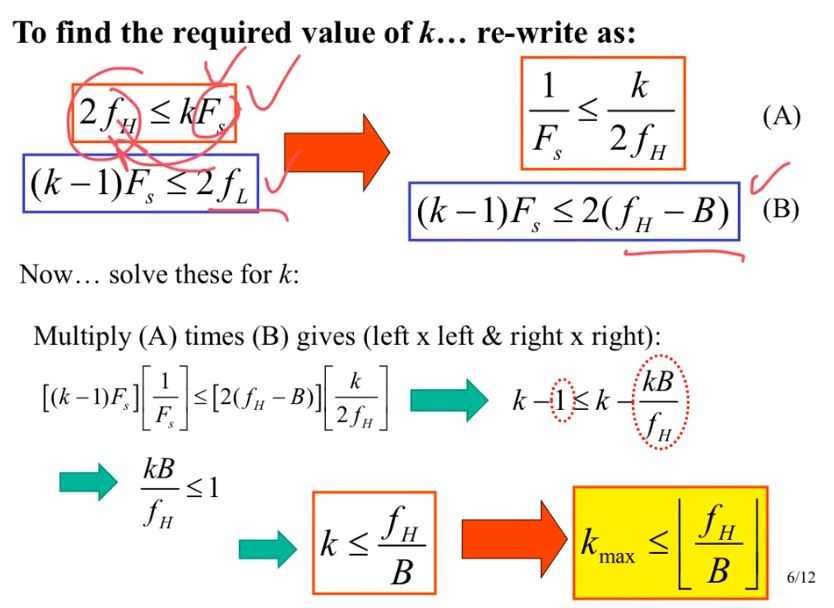
\includegraphics[width = 0.7\textwidth, frame]{Figures/Sampling/bandpass_sampling_general_case_non_integer_bound_k}
\caption{Bandpass sampling non integer case: bounding $k$}
\label{fig:Sampling:bandpass_sampling_general_case_non_integer_bound_k}
\end{figure}


\item As summary:

\begin{equation}
\begin{array}{rcl}
\displaystyle\frac{2 \, f_{\text{high}}}{k} \, &\leq& \, F_s \,\, \, \, \leq \, \displaystyle\frac{2 \,\left( \,  f_{\text{high}} \, - \, \text{Bandwidth} \, \right)}{k \, - \, 1} \\ \\
k \, &\leq& \, \displaystyle\frac{2 \, f_{\text{high}}}{\text{Bandwidth}} 
\end{array}
\label{Eq:Sampling:bandpass_sampling_bounds}
\end{equation}

\newpage
Plotting equations (\ref{Eq:Sampling:bandpass_sampling_bounds}) give us plot shown in \autoref{fig:Sampling:bandpass_sampling_general_case_plots}.


\begin{figure}[h]
\centering
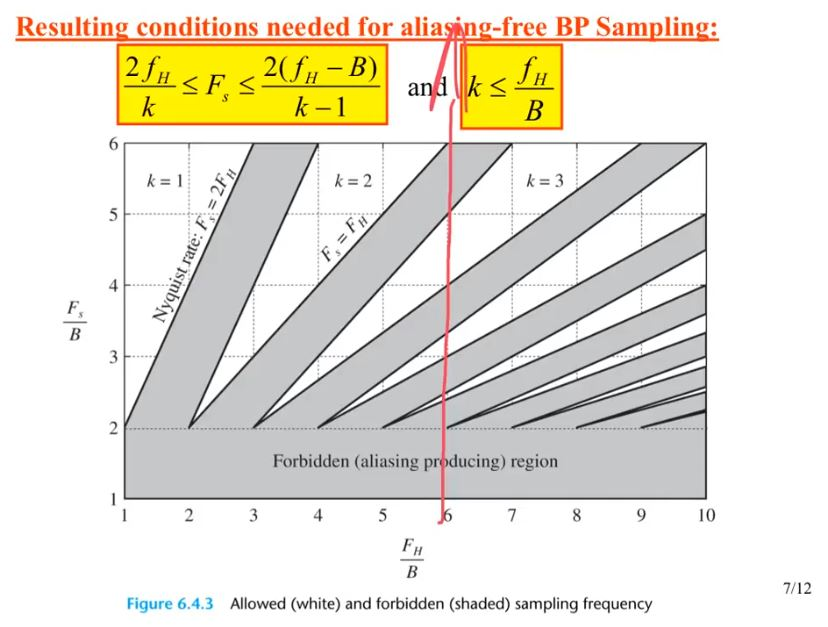
\includegraphics[width = 0.7\textwidth, frame]{Figures/Sampling/bandpass_sampling_general_case_plots}
\caption{Bandpass sampling plot: $F_s$ function of $f_{\text{high}}$}
\label{fig:Sampling:bandpass_sampling_general_case_plots}
\end{figure}

	\begin{itemize}
	\item The plots are normalized over the bandwidth $B$, which makes plotting the equation more easy
	
	\item $k \, = \, 1$: we are operating on the standard Nyquiste rate
	
	
	\item if we have $\displaystyle\frac{f_{\text{high}}}{\text{ bandwidth}} \, = \, 6$, we can operate at multiple $k$: 1,2, 3 and 4 and even 5 (the higher $k$ the lower is $F_s$)
	
	\newpage
	\item However, we have to pay attention at $k \, = \, 5$
	
	\begin{figure}[h]
\centering
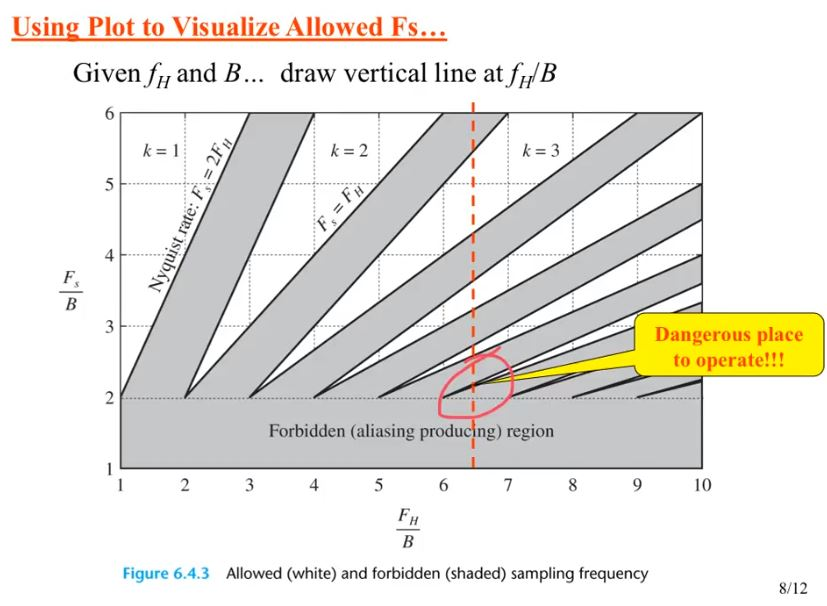
\includegraphics[width = 0.7\textwidth, frame]{Figures/Sampling/bandpass_sampling_general_case_plots_2}
\caption{Bandpass sampling plot: dangerous area we need to pay attention from}
\label{fig:Sampling:bandpass_sampling_general_case_plots_2}
\end{figure}

	\item From this dangerous place, comes the idea of guard band shown in \autoref{fig:Sampling:bandpass_sampling_guard_bands}
	
	
	\begin{figure}[h]
\centering
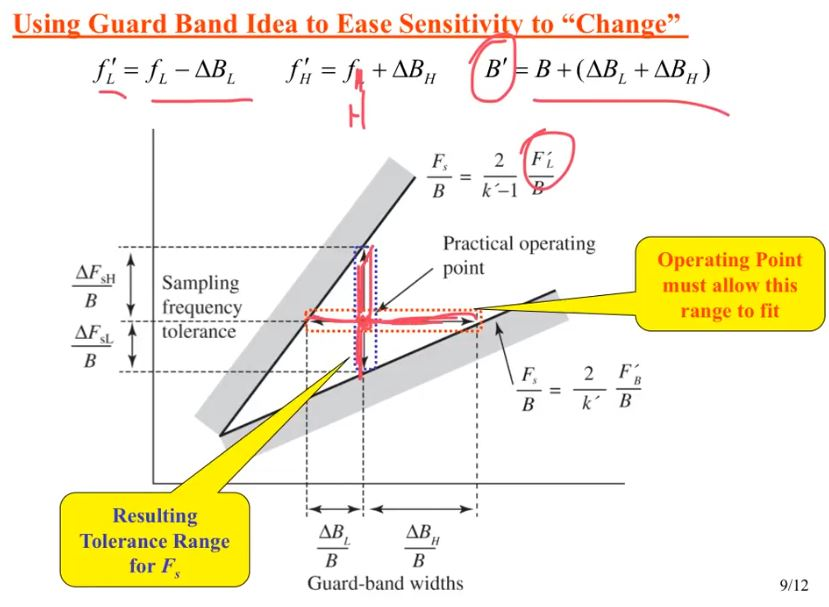
\includegraphics[width = 0.7\textwidth, frame]{Figures/Sampling/bandpass_sampling_guard_bands}
\caption{Bandpass sampling plot:putting some guard bands}
\label{fig:Sampling:bandpass_sampling_guard_bands}
\end{figure}
	
	\end{itemize}

\end{itemize}



\chapter{Convolution}

\section{Introduction}

\todo{Conv Intro} \textit{Conv Intro: To write it down later}.

\section{Definition}

The definition of convolution between 2 signals $x$ and $h$ is:

\begin{equation}
\begin{array}{rcl}

y(t) \, &=& \, \displaystyle \int_{-\infty}^{+\infty} x(\tau) \, h\left(\,t \, - \tau\, \right) d \tau \\ \\

y[k] \, &=& \, x[k] \, * \, h[k] \\ \\
 &=& \displaystyle\sum_{m \, = \, - \, \infty}^{+ \, \infty} x[m] \, h[k \, - \, m] 		
\end{array}
\label{Eq:conv:formula}
\end{equation}

\underline{Notes for \autoref{Eq:conv:formula}:}

\begin{itemize}

\item $h\left(\,t \, - \tau\, \right)$: there is an inversion with respect to time axis (the $-$), then a delay by $t$

    \begin{itemize}
    \item  The integration is with respect to $\tau$, so $\tau$ is the time axis

    \item  The inversion with respect to time, that is  $h(-\tau)$, we flip $h(\tau) \rightarrow$ we have a symmetry (mirror) with respect to $y$ axis
    \end{itemize}

\item  So the shifting will be with respect to $t$ or $m$ in discrete time case: it can be $< \, 0$ or $> \, 0$

    \begin{itemize}
    \item To evaluate the $\displaystyle\int$ or $\displaystyle\sum$ in \autoref{Eq:conv:formula}, we need to take all shifting cases
    \end{itemize}

\end{itemize}

\newpage
\section{Properties}

\underline{Width Property:}\\

$h_1[k]$ has a length of $m_{h_1}$ and $h_2[k]$ has a length of $m_{h_2}$, the resultant signal will have a length of $m_{h_1}  \, + \,m_{h_2} \, - \, 1 $.\\


\underline{Start and Stop time:}\\

\begin{itemize}

\item Start time of $y[k] \, = \, $ start of $x \, + \,$ start of $h$

	\begin{itemize}
	\item Where the start of $x$ and start of $h$ is from the non zero values
	\end{itemize}

\item Stop time of  $y[k] \, = \, $ stop of $x \, + \,$ stop  of $h$

	\begin{itemize}
	\item Where the stop t of $x$ and stop  of $h$ is from the non zero  values
	\end{itemize}

\end{itemize}

\newpage
\section{Example in Continuous Time}

\subsection{Example 1}
\label{sub:ex1_convolution}

Given is shown in \autoref{fig:Convolution:ex1_cont_time}

\begin{figure}[h]
\centering
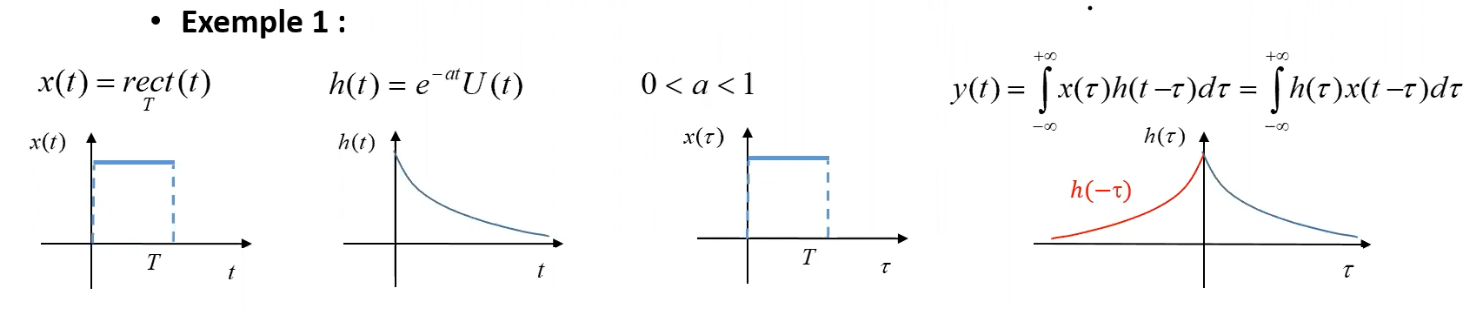
\includegraphics[width = 1.0\textwidth, frame]{Figures/Convolution/ex1_cont_time}
\caption{Example 1 given}
\label{fig:Convolution:ex1_cont_time}
\end{figure}

Before solving, some comments regarding the example:

\begin{itemize}

\item The signal $x(t)$ is time shifted with respect to $T$, it's not like the standard rect function which starts from $\displaystyle\frac{-T}{2} \rightarrow \displaystyle\frac{T}{2}$

\item  Remember that now the new time axis is $\tau$ and not $t$.

    \begin{itemize}
        \item $t$ will act as some constant which can have different cases
    \end{itemize}

\end{itemize}

Now to solve this example, we need to study different time shift cases for $h(\tau)$, but after inversion, that is shifting for $h(-\tau)$. The shifting cases are illustrated in \autoref{fig:Convolution:ex1_time_shift_cases}.

\begin{figure}[h]
\centering
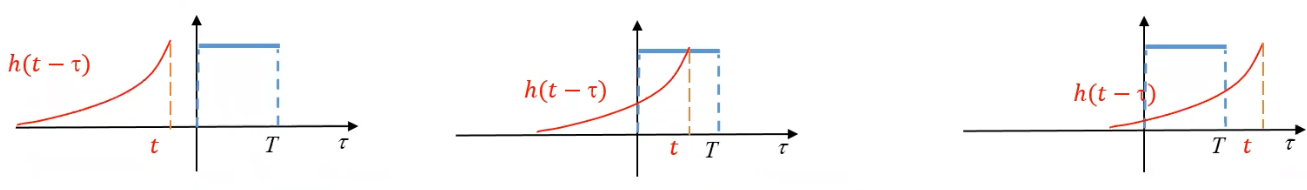
\includegraphics[width = 1.0\textwidth, frame]{Figures/Convolution/ex1_time_shift_cases}
\caption{Example 1 time shifting cases}
\label{fig:Convolution:ex1_time_shift_cases}
\end{figure}

\begin{itemize}

\item Tor $t \, < \, 0$: there is no common area between $x$ and $h$, so $y(t) \, = \, 0$ for $t \, \leq \, 0$

\item  For $t \, > \, 0$:  the signal $x$ finishes at a duration $T$, but $h$ can continue beyond $T$, so in case of $>0$, we distinguish 2 cases: 

    \begin{enumerate}
    \item $0 \,<\, t \, < \, T$:  the boundaries of common surface is from $\tau \, = \, 0 \rightarrow \, \tau \, = \, t$. Using \autoref{Eq:conv:formula}, we have:


$\begin{array}{rcl}
     y(t) &=& \displaystyle \int_{-\infty}^{+\infty} x(\tau) \, h\left(\,t \, - \tau\, \right) d \tau  \\ \\
      &=& \displaystyle \int_{0}^{t} 1 \, \times \, e^{-a \, (t \, - \, \tau)} \, d \tau
\end{array}$

Since the integration is with respect to $\tau$, we can all the non $\tau$ variables ($t$ and $a$) act as constant and we can get them out of the integral

\newpage
$\begin{array}{rcl}
 y(t) &=& e^{-a \, t} \displaystyle \int_{0}^{t} e^{a \, \tau} d\tau \,   \\ \\
    &=& e^{-a \, t}  \left[ \displaystyle\frac{e^{a\tau}}{a} \right]_{0}^{t} \\ \\ 
    &=& \displaystyle\frac{e^{-a \, t}}{a} \, (e^{a \, t} \, - \, 1) \\ \\ 
    &=& \, \displaystyle\frac{1}{a} \, \times \, \left[ \,e^{-a \, t} \, \times \, \left( \, e^{at} \, - \, 1 \,\right) \, \right] \\ \\
    &=& \displaystyle\frac{1}{a} \, \left(\, 1 \, - \, e^{-a \, t}   \, \right)    
\end{array} $\\

\item  $t \, > \, T$: in this case the common area from $\tau \, = \, 0 \rightarrow \, \tau \, = \, T$

Solving we get:\\

$\begin{array}{rcl}
y(t) &=& \displaystyle \int_{-\infty}^{+\infty} x(\tau) \, h\left(\,t \, - \tau\, \right) d \tau  \\ \\
    &=& \displaystyle \int_{0}^{T}  1 \, \times \, e^{-a \, (t \, - \, \tau)} \, d \tau \\ \\
    &=& e^{-a \, t}  \left[ \displaystyle\frac{e^{a\tau}}{a} \right]_{0}^{T} \\ \\ 
    &=& \, \displaystyle\frac{e^{-a \, t}}{a} \, (e^{a \, T} \, - \, 1)
\end{array}$

Rearranging the constant terms we get:


$\begin{array}{rcl}
y(t) \, = \, \left(\, \displaystyle\frac{e^{a \, T} \, - \, 1}{a} \,\right) \, \times \, e^{-a \, t} \text{ for } t \, > \, T
\end{array}$    
    \end{enumerate}

    
\end{itemize}

As a recap, the solution is:

\begin{equation}
y(t) \, = \, 
\begin{cases}
       0 \quad \text{for } t \, < \, 0  \\ \\
        \displaystyle\frac{1}{a} \, \left(\, 1 \, - \, e^{-a \, t}   \, \right) \quad \text{for } 0 \, < \, t \, < T \\ \\
        \left(\, \displaystyle\frac{e^{a \, T} \, - \, 1}{a} \,\right) \, \times \, e^{-a \, t} \text{ for } t \, > \, T
\end{cases} 
\end{equation}



\newpage
\subsection{Example 2}

\underline{Given:} compute the convolution between $x(t)$ and $h(t)$ given in \autoref{Eq:conv:given_ex2}

\begin{equation}
\begin{array}{rcl}
     x(t) &=& \text{some signal}  \quad t \, \in \, ]- \infty \, ,\, - \infty  [   \\ \\
    h(t) &=& \,  \displaystyle\frac{1}{T} \, \text{rect(t)} \quad t \in \left[ \displaystyle\frac{-T}{2} \, , \, \displaystyle\frac{T}{2}  \right]
\end{array}
\label{Eq:conv:given_ex2}
\end{equation}




\underline{Solution:}\\

The signal $x(t)$ is assumed to be some general signal, and the only information we have is the that $x(t)$ exist for all value of $t$.

As for $h(t)$, it is centered at $t \, = \, 0$ , and has a duration $T$ from $\displaystyle\frac{-T}{2} \, \rightarrow \, \displaystyle\frac{T}{2}$.\\

The $\mathrm{1}^\mathrm{st}$ step is always as seen in \ref{sub:ex1_convolution} is the time inversion of $h(\tau)$ with respect to the $y$ axis. Since we have a $\text{rect}(t)$ signal, the inversion will result in the same signal since the rect signal is already symmetric with respect to the $y$ axis.\\

After we have $h(-\tau)$, we start shifting it with different values of $t$. In other words, $h(-\tau)$ is centered at 0, now it will be centered at $t$, and the $t$ can be $< \, 0$ or $>\, 0$, as shown in \autoref{fig:Convolution:rect_shifted}. 

\begin{figure}[h]
\centering
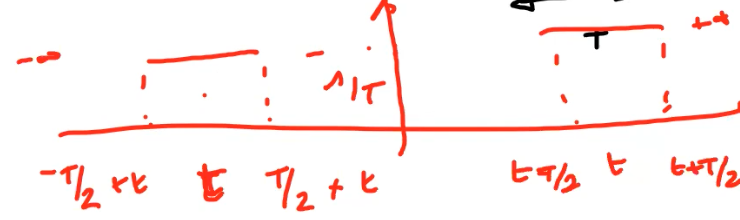
\includegraphics[width = 0.9\textwidth, frame]{Figures/Convolution/rect_shifted}
\caption{Shifting rect signal with different $t$ values}
\label{fig:Convolution:rect_shifted}
\end{figure}

\newpage
Applying \autoref{Eq:conv:formula} for different values of $t$ give the following cases:\\

\underline{$t \, < \, 0$}:


$\begin{array}{rcl}
 y(t) \, &=& \, \displaystyle \int_{-\infty}^{+\infty} x(\tau) \, h\left(\,t \, - \tau\, \right) d \tau  \\ \\
     &=& \, \displaystyle \int_{- \frac{-T}{2} \, + \,t}^{\frac{T}{2} \, + \,t} x(\tau) \, \times \displaystyle\frac{1}{T} \, \times \, 1 \, d\tau \\ \\
     &=& \, \displaystyle\frac{1}{T} \, \int_{- \frac{-T}{2} \, + \,t}^{\frac{T}{2} \, + \,t} x(\tau) \, d\tau
\end{array}$

\underline{$t \, > \, 0$}:\\

For $t \, > \, 0$, we have the same computation since the integral bounds will be the same.\\

The expression $ \displaystyle\frac{1}{T} \, \int_{- \frac{-T}{2} \, + \,t}^{\frac{T}{2} \, + \,t} x(\tau) \, d\tau$ is similar to taking the average of a signal $x(t)$. Recall that the average of a signal $x(t) \, = \, \displaystyle\frac{1}{T} \, \int_{-\frac{-T}{2}}^{\frac{T}{2}} x(t) \, dt$.

So we can say that $\displaystyle\frac{1}{T} \, \int_{- \frac{-T}{2} \, + \,t}^{\frac{T}{2} \, + \,t} x(\tau) \, d\tau$ is taking the average but with different values of $t$. 

That's why $\displaystyle\frac{1}{T} \, \text{rect(t)}$ is called an average filter, since the result of the filtering is taking the average of signal $x(t)$ for all values of $t$.\\

\underline{Note:} see simulation in \verb|MATLAB|.

\newpage
\section{Examples in Discrete Time}

\subsection{Finite Short Signals}
\label{Sub:TimeDomainDiscrete:Example_Short_Signlas}

To do later.


\subsection{Long or Infinite Signal Approach}

In the example of \autoref{Sub:TimeDomainDiscrete:Example_Short_Signlas}, the signals were having few values for some indexes, so the definition of equation (\ref{Eq:conv:formula}) were applicable and we can compute $c[k]$ for each $k$ index. But what if we have some long signals, or some infinite duration signals ? we need a more applicable approach.\\


The method is called \tbi{sliding tapes approach}, where it consist to shift $h[k]$ along the index axis, and compute the $c[k]$ for each time we do the shifting of $h[k]$. The sliding tapes approach can be summarized by doing the following steps:

\begin{enumerate}

\item Plot $f[k]$ and $h[k \, - \, m]$.

\item Shift $h[k \, - \, m]$ to far to the left (large $k$).

\item Multiply and Sum Signals (do the dot product).

\item Shift $k$ until new intermediate signal results.

\item Repeat 3 and 4 until done.

\end{enumerate}

\underline{Example 1:}\\

Let's compute the convolution between:

\begin{itemize}
\item $x[k] \, = \, \alpha^k \, u[k]$, where $0 \, \leq \, \alpha \, \leq \, 1$, so its a damping exponential.

\item $h[k] \, =  \, u[k]$.
\end{itemize}

First, let's recall the definition: $ x[k] \, * \, h[k] \, 
 = \displaystyle\sum_{m \, = \, - \, \infty}^{+ \, \infty} x[m] \, h[k \, - \, m] $.\\

\newpage
We need to able to sketch $x[m]$ and $h[k \, - \, m]$. The sketch is shown in \autoref{fig:Convolution:Example_1_SlidingTapes}.

\begin{figure}[h]
\centering
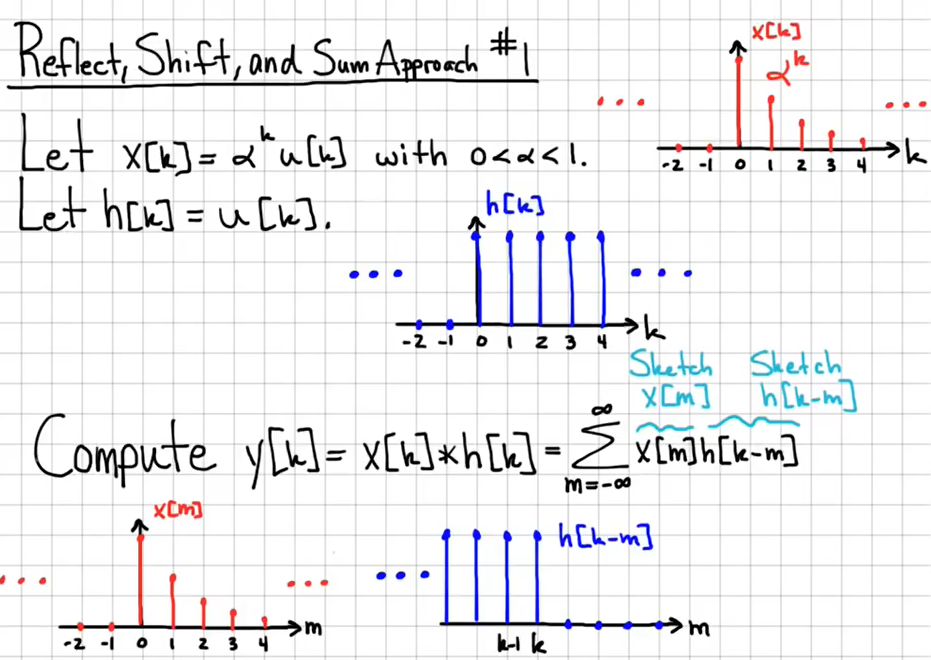
\includegraphics[width = 0.7\textwidth, frame]{Figures/Convolution/Example_1_SlidingTapes}
\caption{Sketching $x[m]$ and $h[k \, - \, m]$}
\label{fig:Convolution:Example_1_SlidingTapes}
\end{figure}

\begin{itemize}

\item $x[m]$ is quite easy because is the same as $x[k]$

\item $h[k \, - \, m]$ is the tricky one: it is a time reversed then shifted signal

	\begin{itemize}
	\item We first do time reversing, so the $h[-m]$ part (reflection with respect to the y axis.)
	
	\item Then we shift to the left
	\end{itemize}

\end{itemize}

The difference between $h[k \, - \, m]$ and $h[k]$ is that:

\begin{itemize}
\item $h[k]$ will turn on at $k \, = \, 0$ and still on until some $k$ value

\item $h[k \, - \, m]$ will be turned off at $k$, so it is the opposite of $h[k]$.
\end{itemize}

It is very important when plotting $h[k \, - \, m]$ to let $k$ be a variable, notice that in \autoref{fig:Convolution:Example_1_SlidingTapes} we didn't specify the origin of $h[k \, - \, m]$, we let it, because for each value of $k$, we will have a different $h[k \, - \, m]$.\\

\newpage
We will study the cases for 2 cases: $k \, < \, 0 $, where we take as example $k \, = \, -2$, and $k \, \geq \, 0$, where $k \, = \, 2$. These cases are shown in \autoref{fig:Convolution:Example_1_SlidingTapes_K_Cases}.

\begin{figure}[h]
\centering
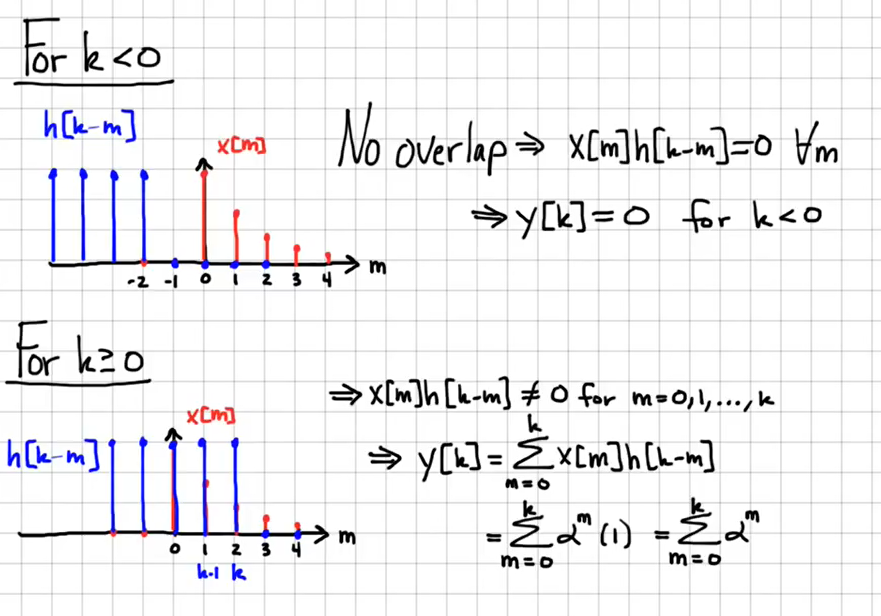
\includegraphics[width = 0.7\textwidth, frame]{Figures/Convolution/Example_1_SlidingTapes_K_Cases}
\caption{$h[k \, - \, m]$ for $k \, < \, 0 $ and $k \, \geq \, 0$}
\label{fig:Convolution:Example_1_SlidingTapes_K_Cases}
\end{figure}

\begin{itemize}

\item For any $k \, < \, 0 $, there will be no overlapping between $h[k \, - \, m]$ and $x[m]$, so the result of the convolution will be 0 for $k \, < \, 0 $.

\item For $k \, \geq \, 0$, there is overlapping between the 2 signals, and this overlapping stop till $k$, so the upper limit of the summation will be till $m \, = \, k$ instead of $m \, = \, + \infty$.

	\begin{itemize}
	\item And sine $x[m] \, = \, 0$ for $m \, < \,0$, so the lower limit of the summation will start from $m \, = \, 0$ instead of $m \, = \, - \infty$.
\end{itemize}	

For  $k \, \geq \, 0$, $h[k \, - \, m] \, = \, 1$.

\end{itemize}


The series for $k \, \geq \, 0$ can be solved using the following formula:

\begin{equation}
\displaystyle\sum_{n \, = \,0}^{N \, - \, 1} \alpha^n \, = \, \begin{cases}
N \quad \text{for } \alpha \, = \, 1 \\ \\
\displaystyle\frac{1 \, - \, \alpha^N}{1 \, - \, \alpha} \quad \text{any complex } \alpha\, \neq \, 1
\end{cases}
\label{Eq:Convolution:Series_Formula}
\end{equation}

\newpage
The computation are shown in \autoref{fig:Convolution:Example_1_SlidingTapes_y}, along with final answer of the convolution $y[k]$.

\begin{figure}[h]
\centering
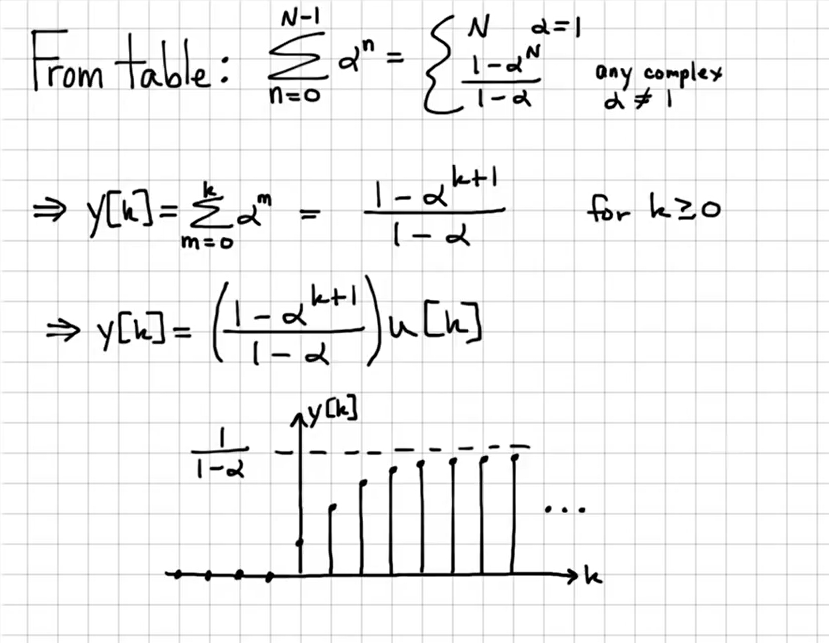
\includegraphics[width = 0.7\textwidth, frame]{Figures/Convolution/Example_1_SlidingTapes_y}
\caption{$y[k]$}
\label{fig:Convolution:Example_1_SlidingTapes_y}
\end{figure}

Notice that when computing $y[k]$, we add $+1$ to $k$, because the formula of equation (\ref{Eq:Convolution:Series_Formula}) add plus 1 to the upper limit $\left( \, N \, - \, 1 \, \right)$. Also the signal $y[k]$ converge to the limit $\displaystyle\frac{1}{1 \, - \, \alpha}$ as $k \, \rightarrow \, + \, \infty$.\\


\underline{Example 2:}\\

Example 2 is shown in \autoref{fig:Convolution:Example_2_SlidingTapes}.

\begin{figure}[h]
\centering
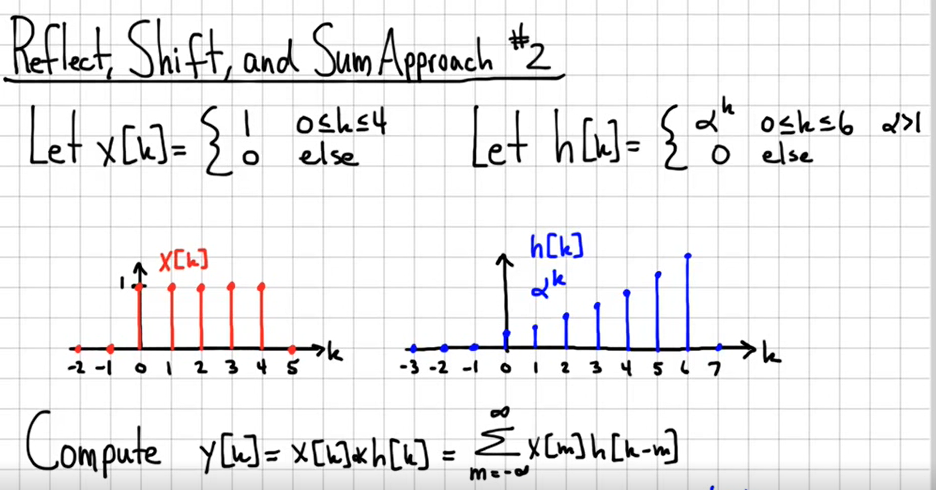
\includegraphics[width = 0.7\textwidth, frame]{Figures/Convolution/Example_2_SlidingTapes}
\caption{Question for Example 2}
\label{fig:Convolution:Example_2_SlidingTapes}
\end{figure}

\newpage
First step is to plot $x[m]$ and $h[k \, - \, m]$. The plot is shown in \autoref{fig:Convolution:Example_2_SlidingTapes_Sketching}.

\begin{figure}[h]
\centering
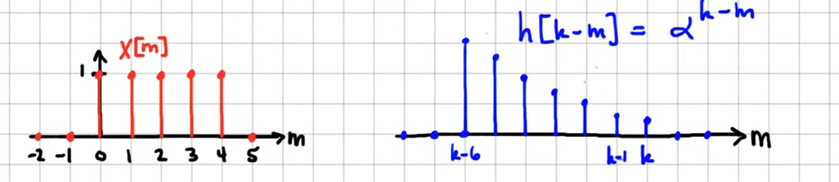
\includegraphics[width = 0.7\textwidth, frame]{Figures/Convolution/Example_2_SlidingTapes_Sketching}
\caption{Sketching $x[m]$ and $h[k \, - \, m]$}
\label{fig:Convolution:Example_2_SlidingTapes_Sketching}
\end{figure}

Again, $h[k \, - \, m]$ is time reversed first and then shifted to the left. We let $k$ to be a variable, and we will study different cases for $k$. Notice that $h[k \, - \, m]$ now start at index $m \, = \, k \, - \, 6$ and stop for index $m \, = \, k$.\\

The approach to compute the solution is the same as in example 1, but here we have more cases to be considered for $k$. All the cases are shown  below from \autoref{fig:Convolution:Example_2_SlidingTapes_Cases_1}  $\rightarrow$ \autoref{fig:Convolution:Example_2_SlidingTapes_Cases_3}.\\


\begin{figure}[h]
\centering
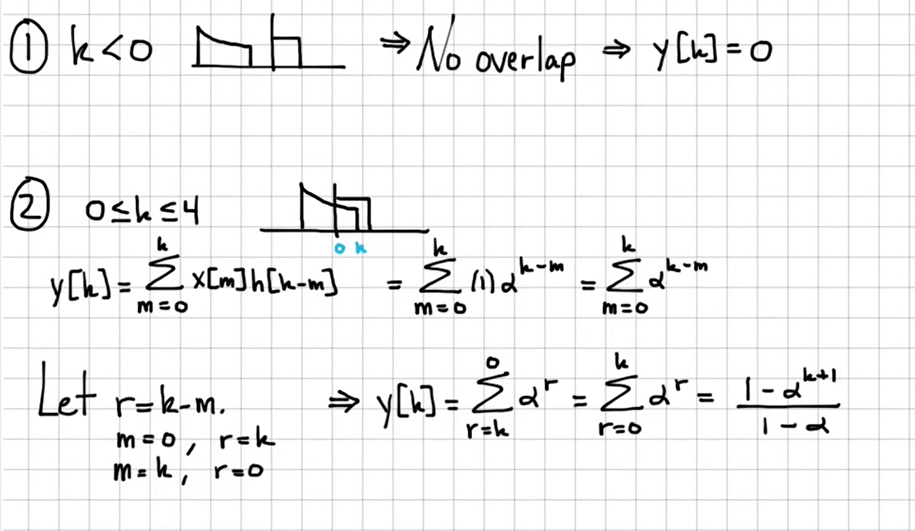
\includegraphics[width = 0.7\textwidth, frame]{Figures/Convolution/Example_2_SlidingTapes_Cases_1}
\caption{$k \, < \, 0$ and $0 \, \leq \, k \, \leq \, 4$}
\label{fig:Convolution:Example_2_SlidingTapes_Cases_1}
\end{figure}


\newpage
In \autoref{fig:Convolution:Example_2_SlidingTapes_Cases_1}, we have made a change of variable $r \, = \, k \, - \, m$ so we can use equation (\ref{Eq:Convolution:Series_Formula}), and also flip the order of series from $\displaystyle\sum_{r \, = \, k}^0 \, \rightarrow \, \displaystyle\sum_{r \, = \, 0}^k$.


\begin{figure}[h]
\centering
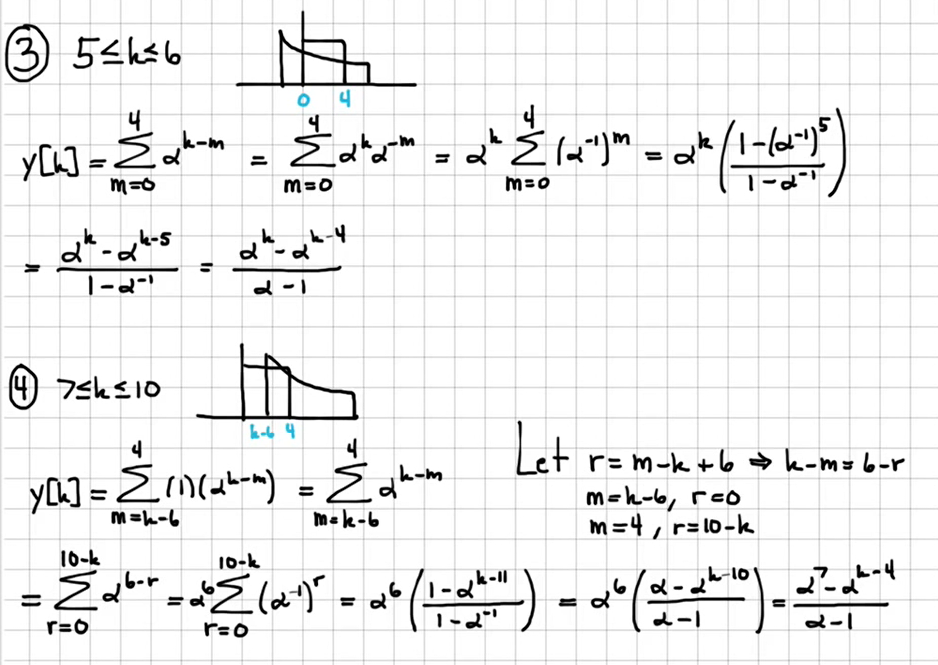
\includegraphics[width = 0.7\textwidth, frame]{Figures/Convolution/Example_2_SlidingTapes_Cases_2}
\caption{$5 \, \leq \, k \, \leq \, 6$ and $7 \, \leq \, k \, \leq \, 10$}
\label{fig:Convolution:Example_2_SlidingTapes_Cases_2}
\end{figure}

\newpage
\begin{figure}[h]
\centering
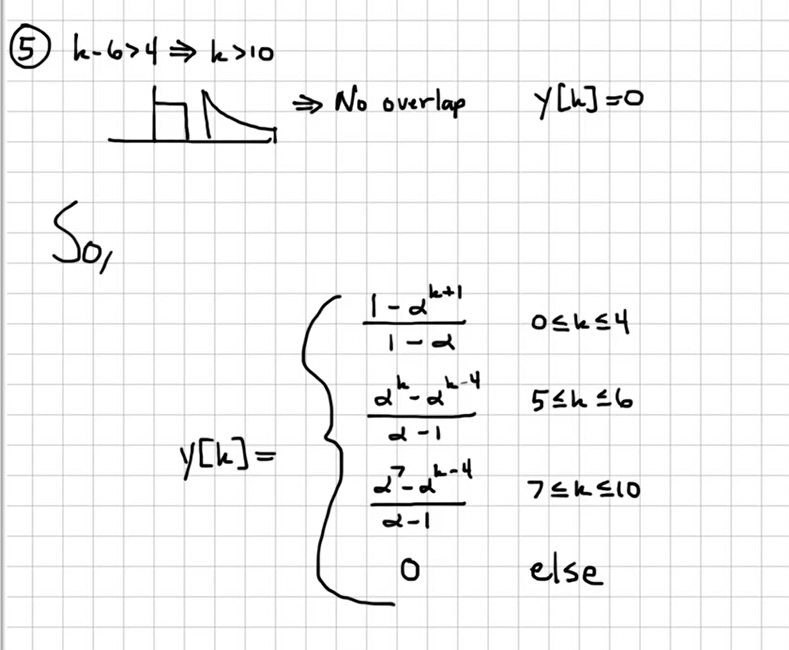
\includegraphics[width = 0.7\textwidth, frame]{Figures/Convolution/Example_2_SlidingTapes_Cases_3}
\caption{$k \, - \, 6 \, > \, 4$ and summing the cases}
\label{fig:Convolution:Example_2_SlidingTapes_Cases_3}
\end{figure}



\chapter{Correlation}

\section{Definition}

First we start by the definition.

\begin{equation}
\begin{array}{lll}
R_{xy}(\tau) \, &=& \, \displaystyle\int_{-\infty}^{\infty} x(t) \, y^\star(t \, - \, \tau) \\ \\
R_{xy}[k]\, &=& \, \displaystyle\sum_{n = -\infty}^{\infty} x[n] \, y^\star[n \, - \, k] 
\end{array}
\end{equation}

Some points:

\begin{itemize}

\item We note that with respect to a convolution, the $\mathrm{2}^\mathrm{nd}$ signal $y(t)$ is only delayed in time by $\tau$, and there is no time flipping operation (in convolution, we have the 2).

\item For a periodic signal with a period $N$, the $R_{xy}[k]$ will be also periodic.

\item Length of signal:

    \begin{itemize}
        
        \item Crosscorrolation: length $x[n] \, = \, N$ , length $y[n] \, = \, M$, we have the $R_{xy}[k]$ length equal to $N + M - 1$ 

        
        \item For autocorollation: for a length $N \rightarrow 2\, N \, - \, 1$

        
    \end{itemize}

\end{itemize}



\chapter{Discrete Time Fourier Transform}


\section{Relation between DTFT and impulse sampled CTFT}


\begin{equation}
\begin{array}{rcl}
\omega_c \left(\text{rad/sec}\right) \, &=& \, \omega_d \, \times \, F_s \\ \\
&=& \, \displaystyle\frac{\omega_d}{T_s} 
\end{array}
\end{equation}




%*****************************************************
%*****************************************************
%*****************************************************


\chapter{The Discrete Fourier Transform}

\section{Introduction}

The discrete Fourier transform is a \tbi{numerical technique} which computes the DTFT (discrete time Fourier transform) and CTFT (continuous time Fourier transform). In other words, there is \tbi{no transformation from time to frequency domain}.


\section{Formula and Direct Results}

\underline{Goal:} Compute Numerically DTFT and CTFT. We start by DTFT.\\

\underline{Note:} To see the derivation, review the slides.


\subsection{Discrete time case: DFT of DTFT}

Let $f[k]$ a discrete signal with index $k$, of length $N_0$.


\begin{equation}
\begin{array}{rcl}
\text{DFT}\{f[k]\} \, &=&\, F_r \\
						&=& \, F(r \, \Omega_0) \\
					   &=&\, \displaystyle\sum_{k \, = \, 0}^{N_0 \, - \, 1} \, f[k] \, \text{exp} \left(\, -j r \Omega_0 \, k   \,\right)
\end{array}
\label{Eq:DFT:dft_for_dtft}
\end{equation}
 
where $\begin{cases}
r \, = \, 0,1,2, \rightarrow \, N_0 \, - \, 1 \\
\Omega_0 \, = \,  \displaystyle\frac{2 \, \pi}{N_0} \, = \, \text{freqeuncy step at which we sample the DTFT spectrum}
\end{cases}$\\


\underline{Inverse DFT case:}\\

\begin{equation}
\begin{array}{rcl}
f[k] \, &=&\, \displaystyle\frac{1}{N_0} \, \displaystyle\sum_{r \, = \, 0}^{N_0 \, - \, 1} \, F_r \, \text{exp} \left(\, -j r \Omega_0 \, k   \,\right)
\end{array}
\end{equation}

\newpage
\subsection{Continuous time case: DFT of CTFT}

\begin{itemize}

\item Let $f(t)$ be a continuous time signal of duration $\tau$.

\item Sample the signal $f(t)$ over a period $T_0 \, \leq \, \tau$, where $T_s$ is the sampling time. 

	\begin{itemize}
	\item The \tbi{number of sample} we get is $N_0 \, = \, \displaystyle\frac{T_0}{T_s} \, = \, T_0 \, \times \, F_s$
	\end{itemize}

\item Formula:

\begin{equation}
\begin{array}{rcl}
\text{DFT}\{f[t]\} \, &=&\, F_r \\
						&=& \, F(r \, \omega_0) \\
					   &=&\, \displaystyle\sum_{k \, = \, 0}^{N_0 \, - \, 1} \, f_k \, \text{exp} \left(\, -j r \Omega_0 \, k   \,\right)
\end{array}
\end{equation}

where $\begin{cases}

\omega_0 \, = \, 2 \, \pi \, F_0 \, \text{rad/s} \, (\text{from spectral sampling theorem}) \\
\Omega_0 \, = \, \omega_0 \, T_s \, = \,   \displaystyle\frac{2 \, \pi}{N_0} \, = \, \text{sampling interval at wihich we sample the spectrum of the CTFT} \\
f_k \, = \, T_s \, f(k \, T_s)
\end{cases}$ 



\end{itemize}


\section{Examples}

\subsection{Continuous time case: Infinite Time}
\label{Sub:DFT:Continuous_time_Infinite_Time}

The signal is: $x(t) \, = \, \text{exp}(-0.5 \, t) \, u(t) \leftrightarrow \, X(\omega) \, = \, \displaystyle\frac{1}{j \, \omega\, + \, 0.5}$.\\

The Fourier transform can be found by any look up table.


\begin{figure}[h]
\centering
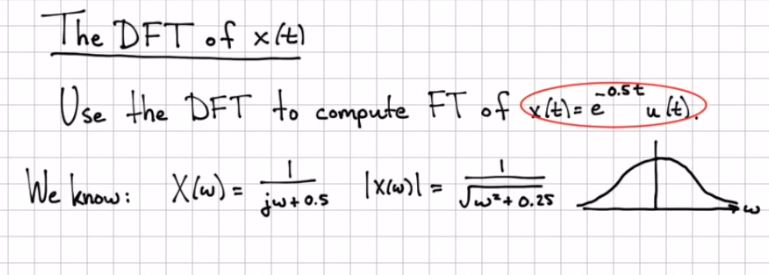
\includegraphics[width = 0.7\textwidth, frame]{Figures/DFT/example_cont_time}
\caption{Given: Infinite time and infinite frequency signal}
\label{fig:DFT:example_cont_time}
\end{figure}


\begin{itemize}

\item To compute the DFT, we need to sample in the time domain ($f_k$) , and take samples in the frequency domain ($\Omega_0$).

\item However $x(t)$ in infinite in time and hence infinite in frequency, and there is no max frequency to apply the sampling period to.

	\begin{itemize}
	\item Need to do some engineering judgment about this.
	\end{itemize}

\item We can put the following criteria: what is the value of $\omega$ at which the frequency content is bellow 2 \% ?

	\begin{itemize}
	\item So we capture 98 \% of the frequency content of the signal
	
	\item This value of $\omega \, = \, 50 \text{rad/s} \leftrightarrow \, B \, = \,  \displaystyle\frac{25}{\pi}$ Hz as shown in \autoref{fig:DFT:capture_sampling_period}
	
\begin{figure}[h]
\centering
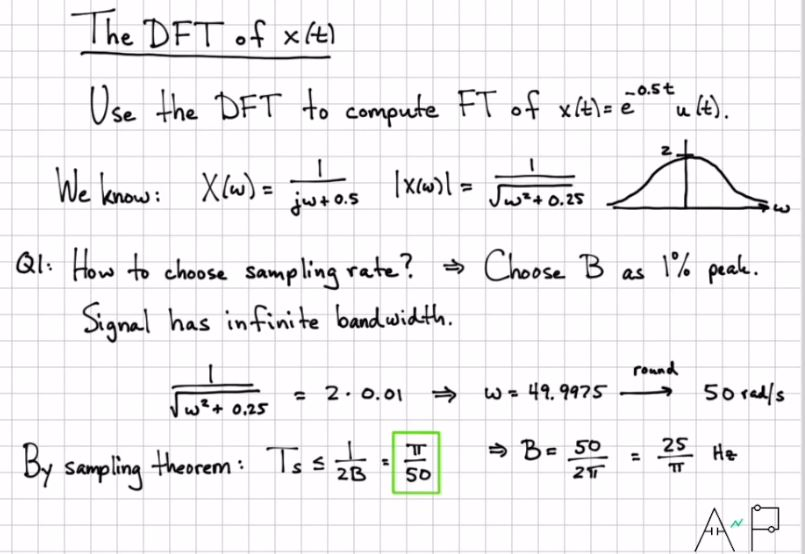
\includegraphics[width = 0.7\textwidth, frame]{Figures/DFT/capture_sampling_period}
\caption{Solving for the sampling period $T_s$}
\label{fig:DFT:capture_sampling_period}
\end{figure}

	\item The we solve for the $T_s$ and we get that we need to sample at a rate $\displaystyle\frac{\pi}{50}$ seconds (this the minimum, we could sample faster, we see the effect of this later) 
	
	\end{itemize}

\item After we solve for $T_s \, = \, \displaystyle\frac{\pi}{50}$ s, there is another question to be asked: for \tbi{how long do we need to sample}?

	\begin{itemize}
	\item This signal is going forever, we can't just keep sampling forever
	\end{itemize}

\item So we need to solve for $T_0$

\newpage
\item We know that the signal is a decaying exponential, we can see for some value of $T_0$ where the amplitude value of $x(t)$ are very low, and by this we are not throwing some high value amplitude (information)

\item Computation shown in \autoref{fig:DFT:when_stop_sample}.

\begin{figure}[h]
\centering
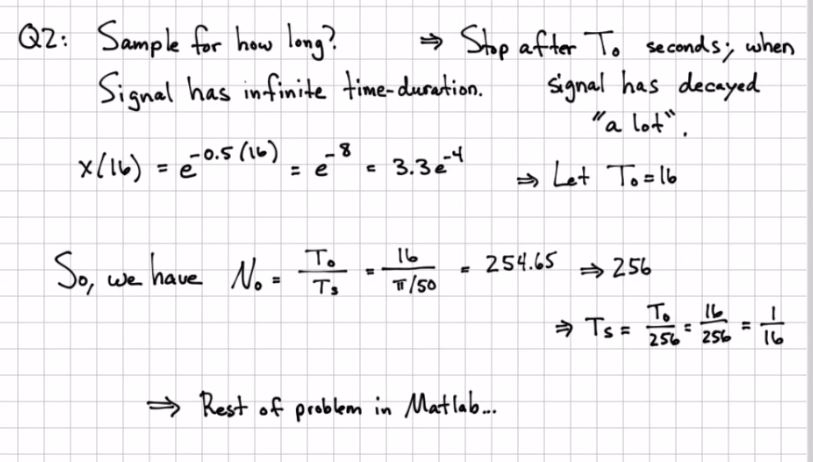
\includegraphics[width = 0.7\textwidth, frame]{Figures/DFT/when_stop_sample}
\caption{Solving for the sampling period $T_s$}
\label{fig:DFT:when_stop_sample}
\end{figure}

	\begin{itemize}
	\item We try for example for $T_0 \, = \, 16$s, we get $x(16) \, = \, 3.3 \, e^-4$, very small number
	
	\item If we choose $T_0 \, = \, 16$, the number of sample we get in this period using a sampling rate $T_s \, = \, \displaystyle\frac{\pi}{50}$ is: $N_0 \, = \, \displaystyle\frac{T_0}{T_s} \, = \, 254.65$
	
	
	\item However, the number of samples we need to grab need to be integer, so let's say we need to grab 256 samples
	
	\item We resolve again for $T_s$ using $N_0 \, = \, 256$ samples, and we get $T_s \, = \, \displaystyle\frac{1}{16}$ seconds
	
	\end{itemize}

\end{itemize}


The rest of the problem is done via coding.


As a summary we have:

\begin{itemize}

\item First question we ask since the signal $x(t)$ isn't band limited in the frequency domain: how do we choose the sampling rate $T_s$

	\begin{itemize}
	\item $T_s \, = \, \displaystyle\frac{1}{16}$ seconds
	\end{itemize}
	
\item $\mathrm{2}^\mathrm{nd}$ question: for how long we keep sampling ?

	\begin{itemize}
	\item $T_0 \, = \, 16$ s, which give $N_0 \, = \, 256$ samples/second
	such that $T_s \, = \, \displaystyle\frac{1}{16}$ s
	\end{itemize}

\end{itemize}


\underline{Some Tuning and Analysis:}\\

2 factors influence the results of the DFT values: the sampling period $T_s$ and signal duration $T_0$, which specify for how long we keep doing sampling. Let's try to change each factor while fixing the other.\\

\underline{Changing signal duration $T_0$:}\\


The results of the computation are shown in \autoref{fig:DFT:cont_time_signal_duration}.

\begin{itemize}

\item The base line is the first row where $F_s \, = \, 16 \text{ sample}/\,\text{s}$ and $T_0 \, = \, 16$s, as in the theoretical part

\item First we truncate (throw away) the signal allot, which means $T_0$ decrease (decrease to 2 s in our choice)

	\begin{itemize}
	\item Since $\Omega_0 \, = \, \displaystyle\frac{2 \, \pi}{N_0}$ and $N_0 \, = \, \displaystyle\frac{T_0}{T_s}$, so we get less number of coefficient for DFT computation
	
	\item And notice that the values of the DFT in the $\mathrm{2}^\mathrm{nd}$ plot are below the blue curve
	\end{itemize}	 

\item When we increase the signal duration (truncate less) things tend to be better.

\end{itemize}

As a conclusion, even if the sampling rate $F_s$ is good enough but we truncate the signal allot in the time domain, the spectral representation will not be good and we loss frequency content of the signal.

\begin{figure}[h]
\centering
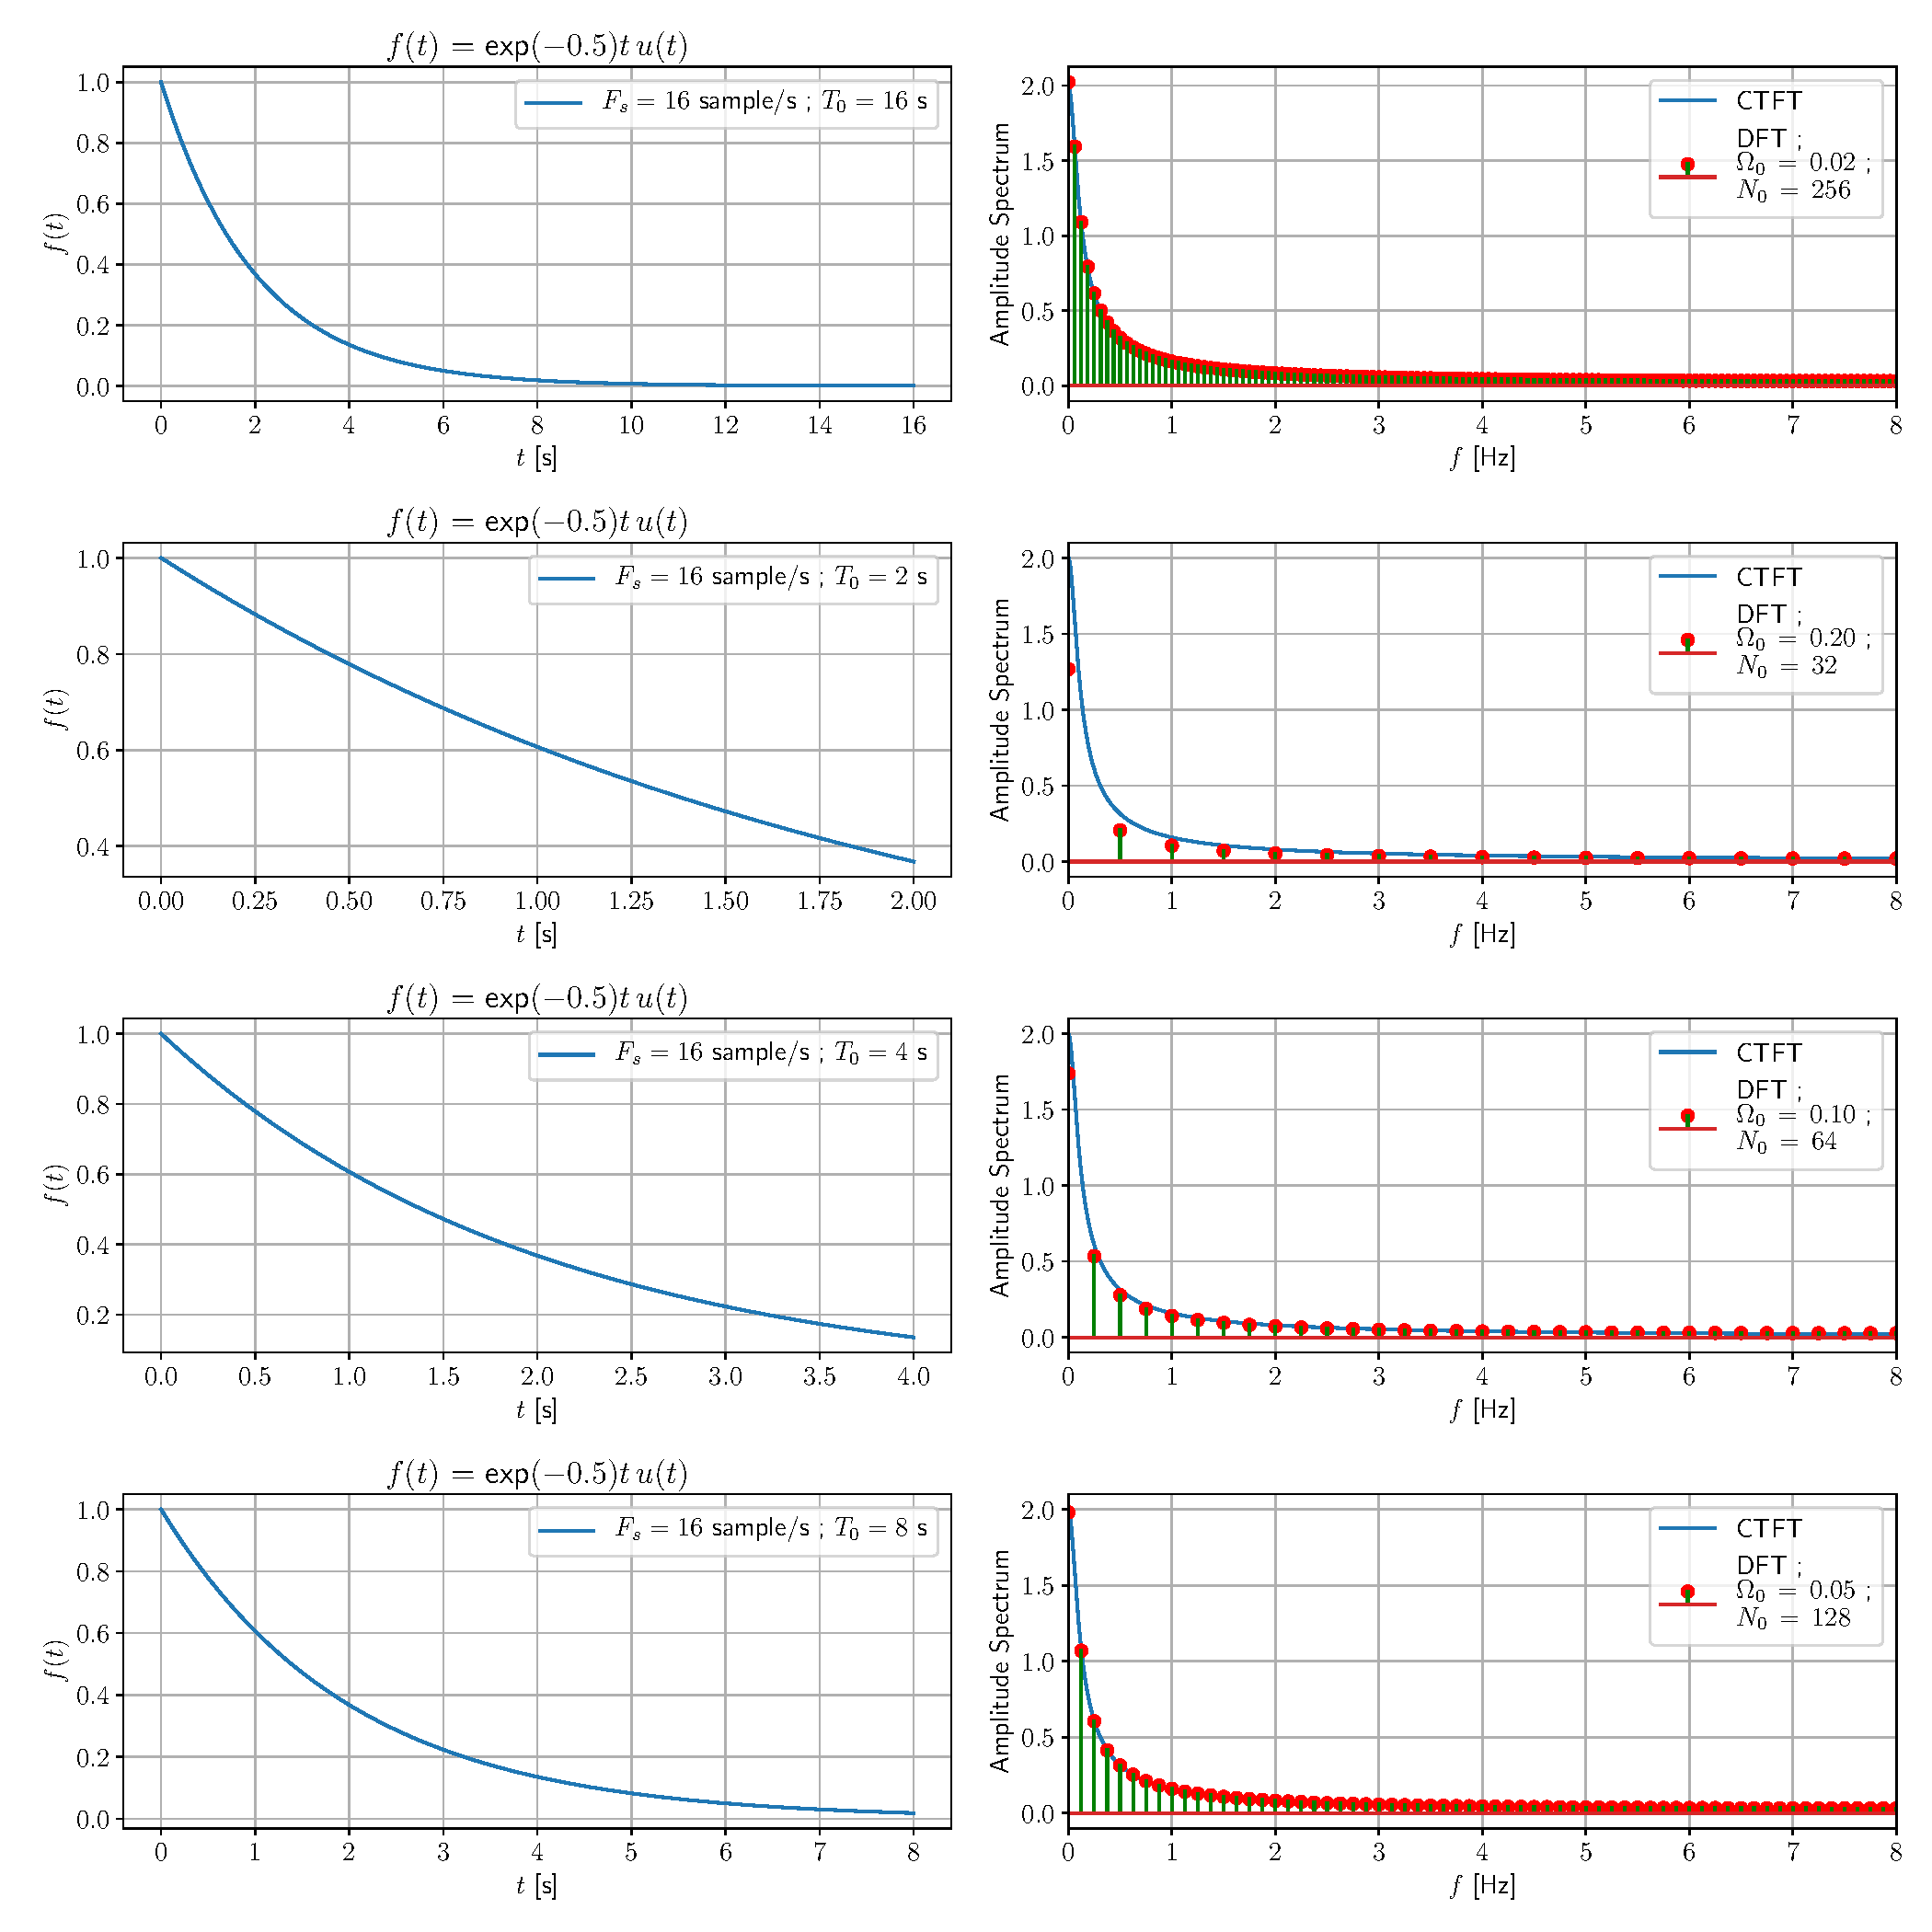
\includegraphics[width = 0.7\textwidth, frame]{Figures/DFT/DFT_Continous_time_signal_duration}
\caption{DFT results for example of \autoref{fig:DFT:example_cont_time}: Signal Duration $T_0$ and its effect on DFT}
\label{fig:DFT:cont_time_signal_duration}
\end{figure}

\newpage
\underline{Changing the sampling rate $F_s$:}\\

Results are shown in \autoref{fig:DFT:cont_time_sampling_rate}.

\begin{figure}[h]
\centering
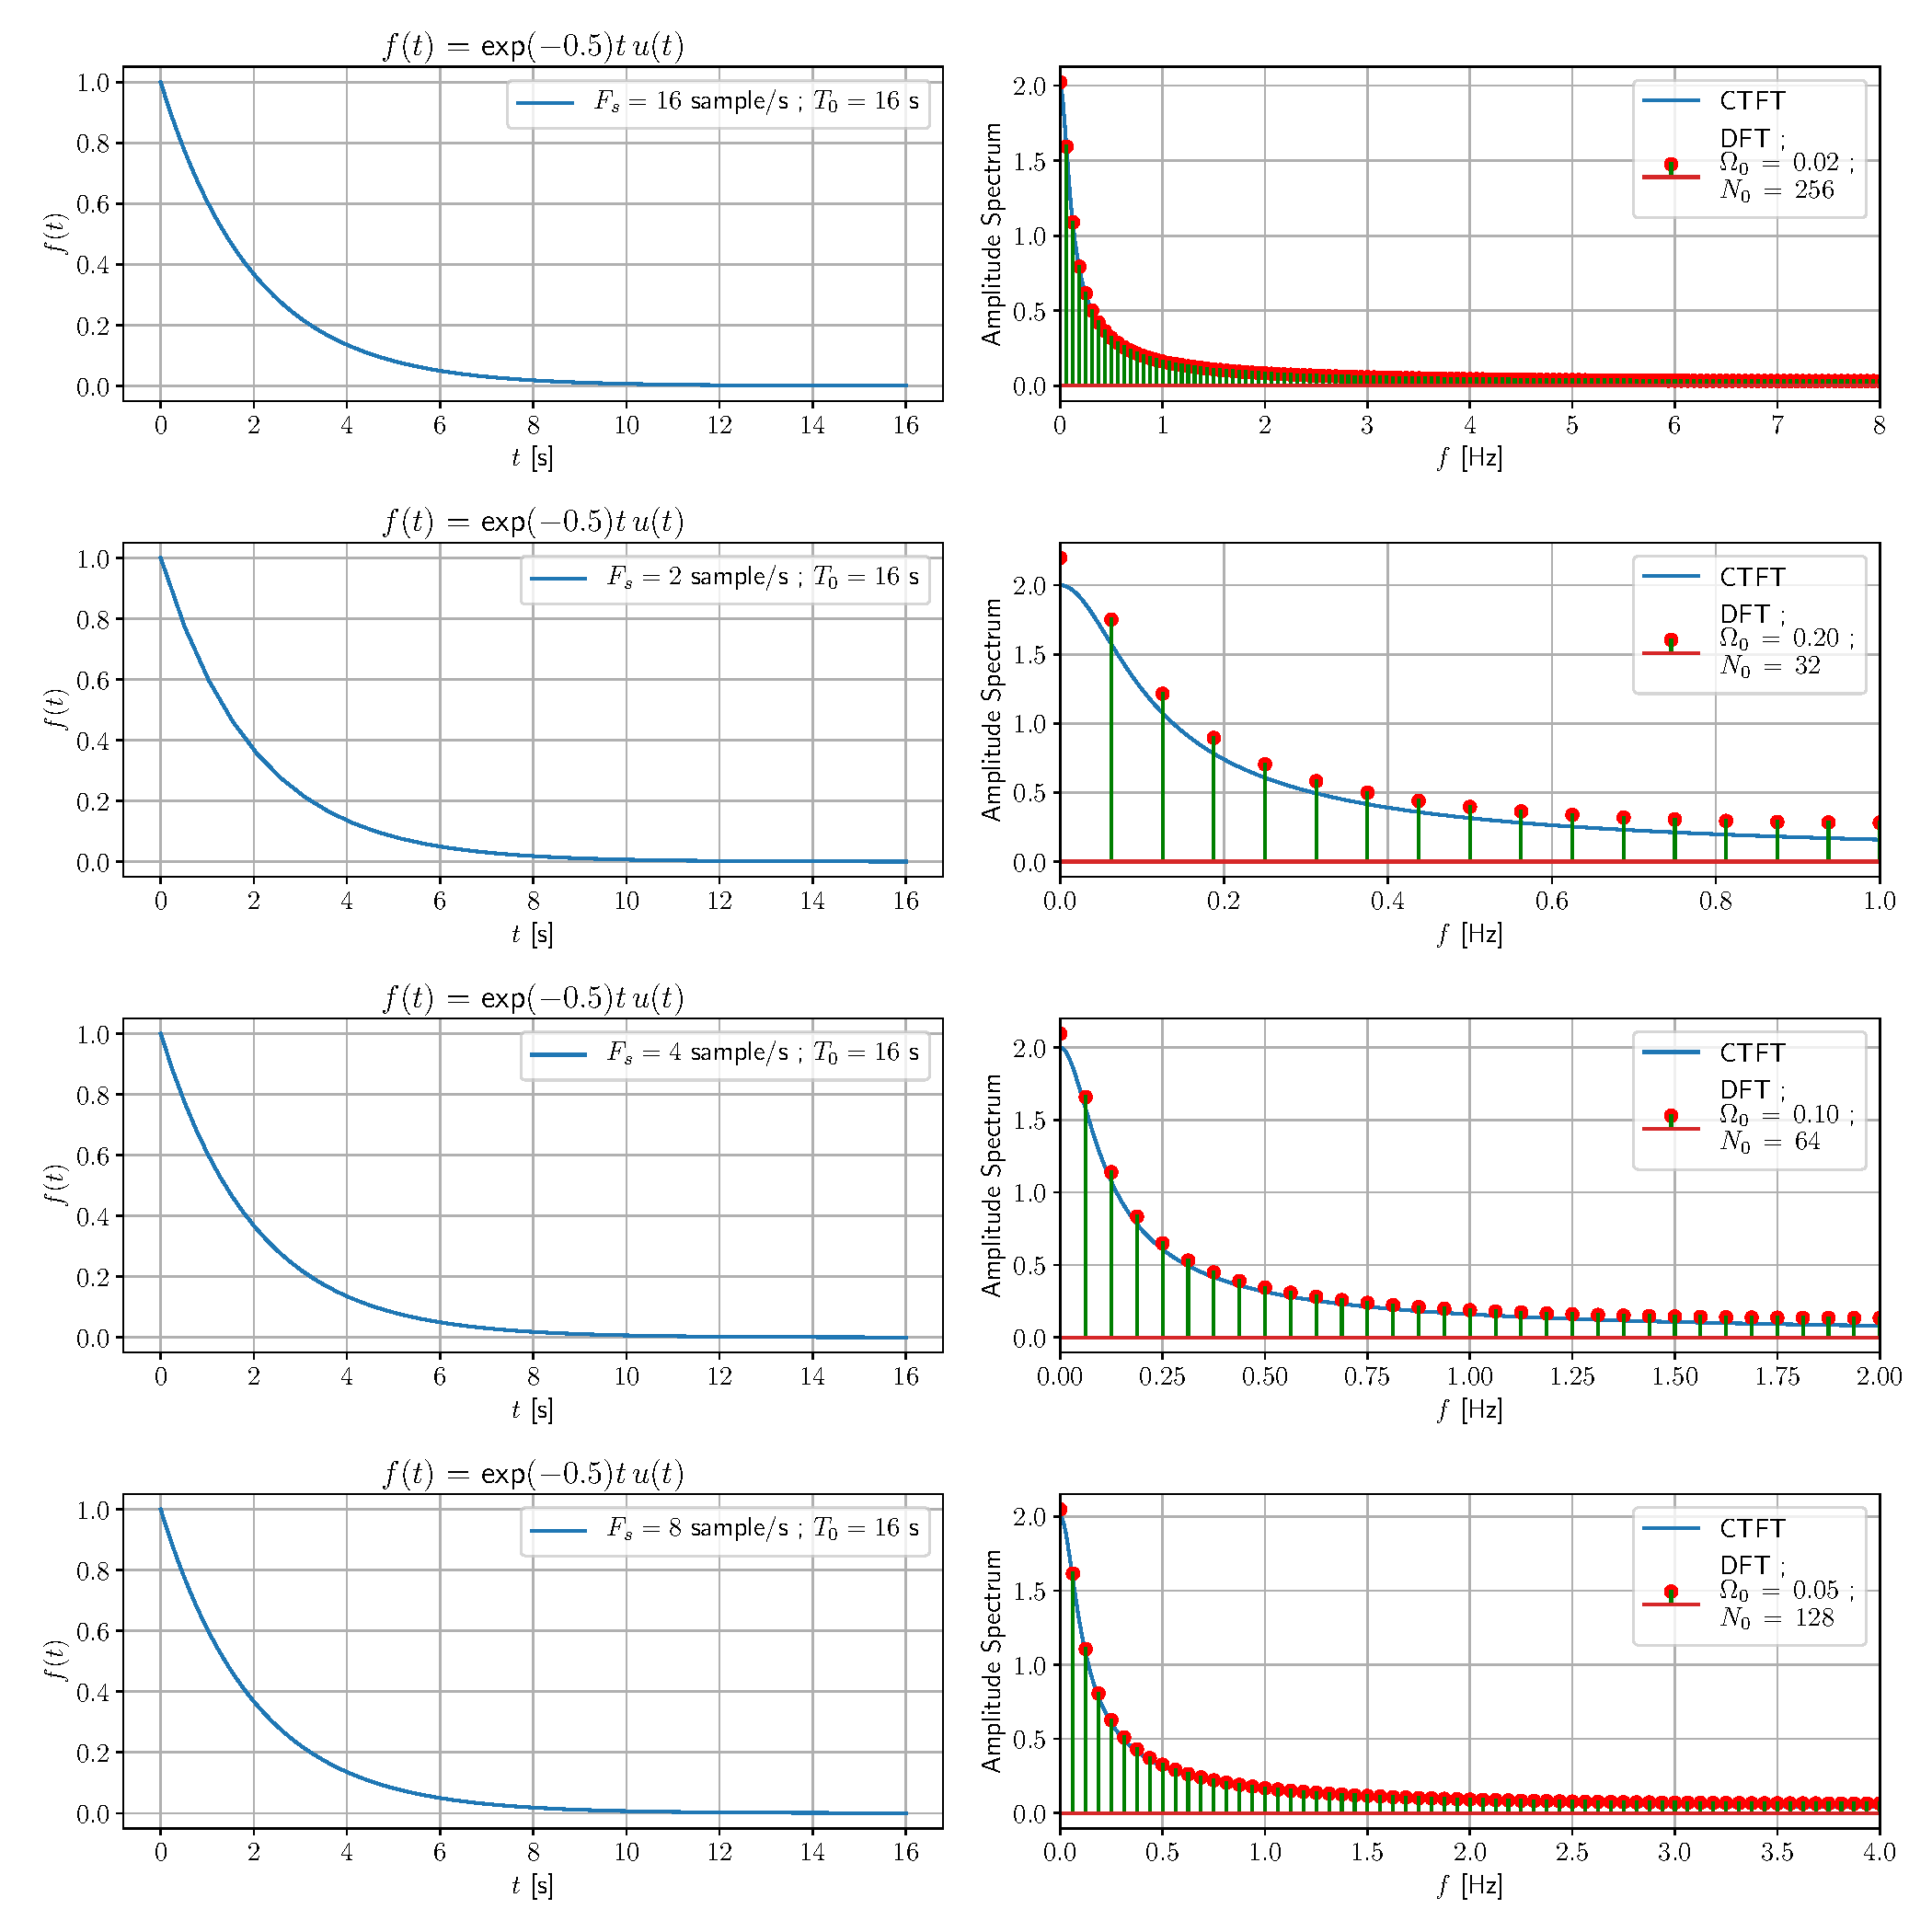
\includegraphics[width = 0.7\textwidth, frame]{Figures/DFT/DFT_Continous_time_sampling_rate}
\caption{DFT results for example of \autoref{fig:DFT:example_cont_time}: Sampling rate $F_s$ and its effect on DFT}
\label{fig:DFT:cont_time_sampling_rate}
\end{figure}

\begin{itemize}

\item As usual the first plot is the base line: $F_s \, = \, 16 \text{ sample/s}$ and $T_0 \, = \, 16$s.

\item Notice that for example when $F_s \, = \, 2 \text{ sample/s}$ (8 times less than the true one), the DFT values are above the true curve of the CTFT.

\end{itemize}



\newpage
\subsection{Discrete Time: Finite Length Signal}

The problem is shown in \autoref{fig:DFT:discrete_case_finite_length}.

\begin{figure}[h]
\centering
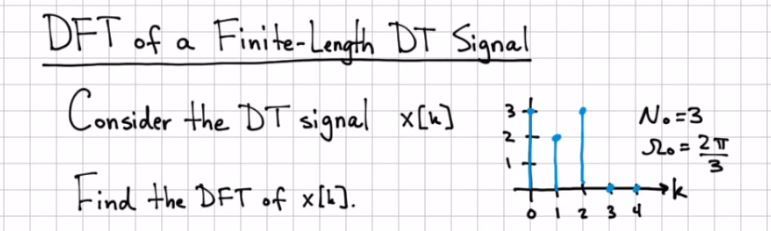
\includegraphics[width = 0.7\textwidth, frame]{Figures/DFT/discrete_case_finite_length}
\caption{Discrete time signal: finite length}
\label{fig:DFT:discrete_case_finite_length}
\end{figure}

\begin{itemize}

\item It has 3 non-zero values at indices 0,1 and 2, so $N_0 \, = \, 3$

\item Since $N_0 \, = \, 3$, so the DFT components for the DTFT will be also 3: $r: 0 \, \rightarrow \, 2$

\item The \tbi{sampling interval} at which we compute the DFT coefficient values is $\Omega_0 \, = \, \displaystyle\frac{2\, \pi}{N_0} \, = \, \displaystyle\frac{2\, \pi}{3}$

	\begin{itemize}
	\item So we compute the value at $0 \, \Omega_0 \, , 1 \, \Omega_0\,$ and $2 \, \Omega_0 $
	\end{itemize}

\end{itemize}


Since the values of the DFT are only 3, we can do the computation by hand easily using equation (\ref{Eq:DFT:dft_for_dtft}). The computations are shown in \autoref{fig:DFT:discrete_case_finite_length_computation} 


\begin{figure}[h]
\centering
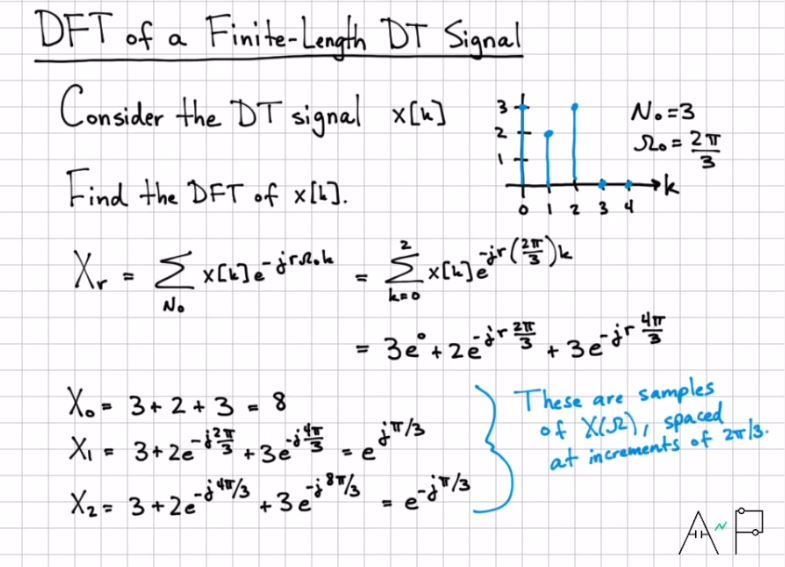
\includegraphics[width = 0.7\textwidth, frame]{Figures/DFT/discrete_case_finite_length_computation}
\caption{Computing DFT values of the DTFT using equation (\ref{Eq:DFT:dft_for_dtft})}
\label{fig:DFT:discrete_case_finite_length_computation}
\end{figure}

	\begin{itemize}
	\item First we compute a formula as a function of $r$ for all values of time index $k$
	
	\item Then we plug each value of $r$ to obtain $X_0 \, , \, X_1$ and $X_2$
	\end{itemize}

\newpage
Now to compare the result of the DFT values, we compute also the expression of DTFT, detailed in \autoref{fig:DFT:dtft_expression}.

\begin{figure}[h]
\centering
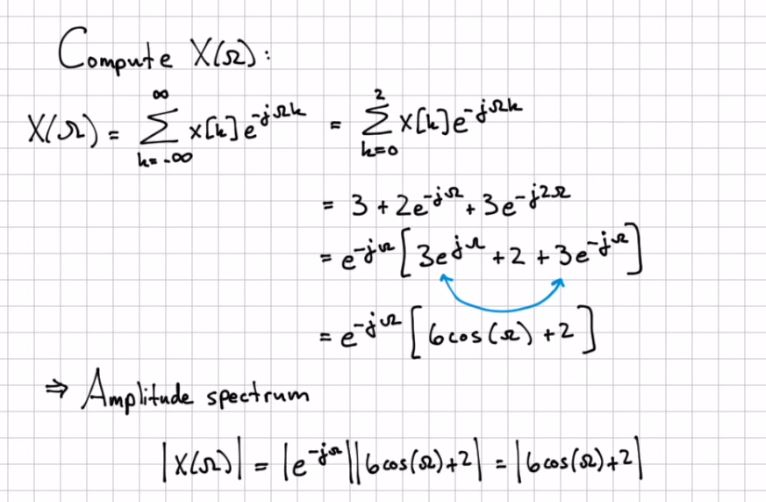
\includegraphics[width = 0.7\textwidth, frame]{Figures/DFT/dtft_expression}
\caption{Computing DTFT expression for comparison with DFT values}
\label{fig:DFT:dtft_expression}
\end{figure}

\newpage
\underline{Results and Analysis:}\\

Results are shown in \autoref{fig:DFT:discrete_case_finite_length_results}.

\begin{figure}[h]
\centering
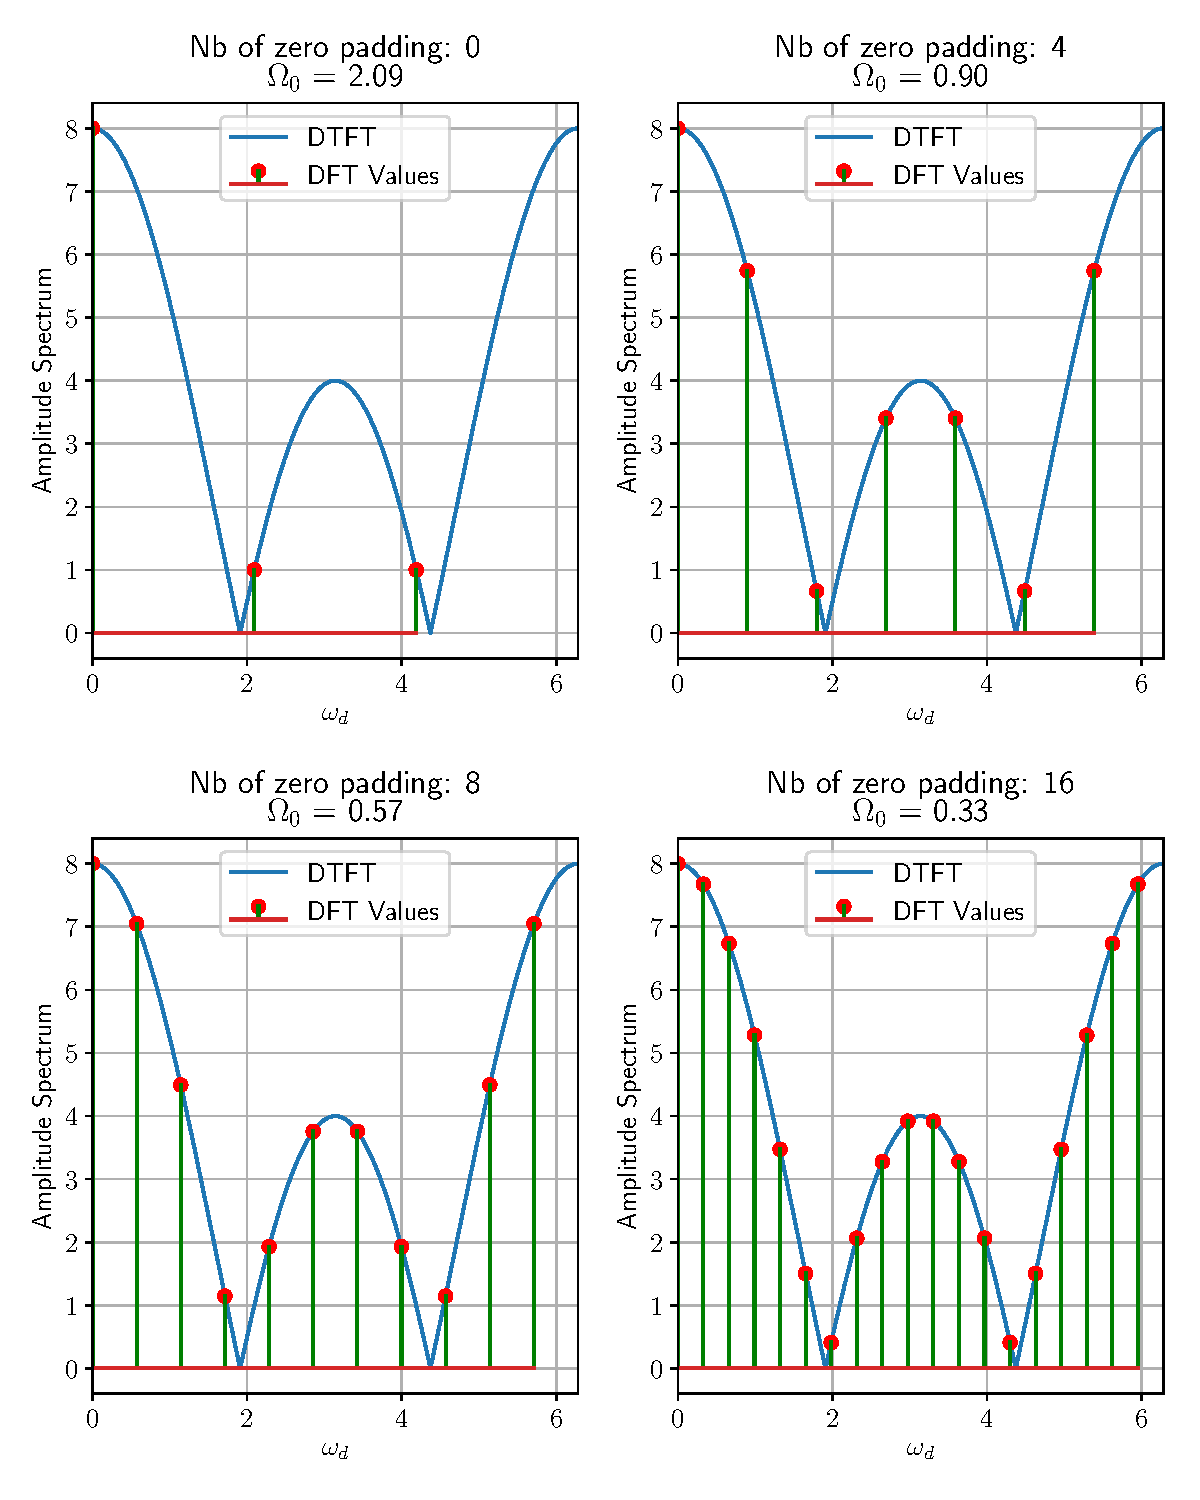
\includegraphics[width = 0.7\textwidth, frame]{Figures/DFT/DFT_Discrete_time_Finite_Length}
\caption{Results of Example of  \autoref{fig:DFT:discrete_case_finite_length} \\ $ 0 \, \leq \,  \omega_d \leq \, 2 \, \pi$}
\label{fig:DFT:discrete_case_finite_length_results}
\end{figure}

\begin{itemize}

\item The result are also made with respect to \tbi{zero padding} effect

	\begin{itemize}
	\item We pad (add) zeros values to the signal in the time (discrete) domain
	
	\item This won't affect the signal, only the number of samples will increase
	
	\end{itemize}

	\item Recall that the sampling interval $\Omega_0 \, = \, \displaystyle\frac{2\, \pi}{N_0}$ where $N_0$ is the length of the signal
	
	\item If we add more samples $N_0$, $\Omega_0$ will decrease and hence we take more samples of the spectrum of the DTFT.

\end{itemize}

\newpage
\subsection{Discrete Time: Infinite Length Signal}

Now we move with infinite length discrete time signal. As in \ref{Sub:DFT:Continuous_time_Infinite_Time}, since we are dealing with infinite length sequence, we need to truncate the signal in the time (discrete) domain and make the index sampling $k$ between 0 and $N_0 \, - 1$. Given are shown in \autoref{fig:DFT:discrete_case_Infinite_length_given}

\begin{figure}[h]
\centering
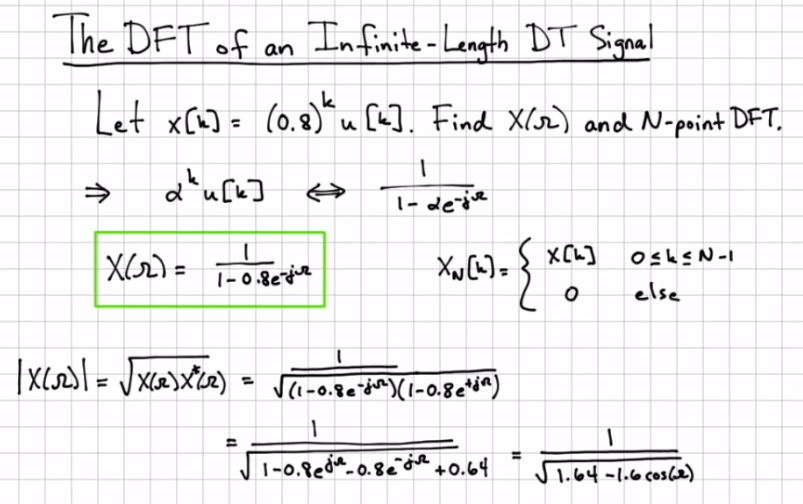
\includegraphics[width = 0.7\textwidth, frame]{Figures/DFT/DFT_Discrete_time_Infinite_Length_given}
\caption{DFT for infinite length discrete time signal}
\label{fig:DFT:discrete_case_Infinite_length_given}
\end{figure}

Results are shown in \autoref{fig:DFT:discrete_case_Infinite_length_results}.

\begin{itemize}

\item $k$ is the sampling index in the discrete time domain

\item The base $a \, = \, 0.8$ in all cases

\item $p$ is the number of samples we get:

	\begin{itemize}
	\item The more $p$ we get, the \tbi{less we truncate the signal in the discrete time domain}, and hence the DTFT using the loop formula and the DFT values will get more accurate to analytical DTFT formula
	\end{itemize}

\end{itemize}
 
\newpage
\begin{figure}[h]
\centering
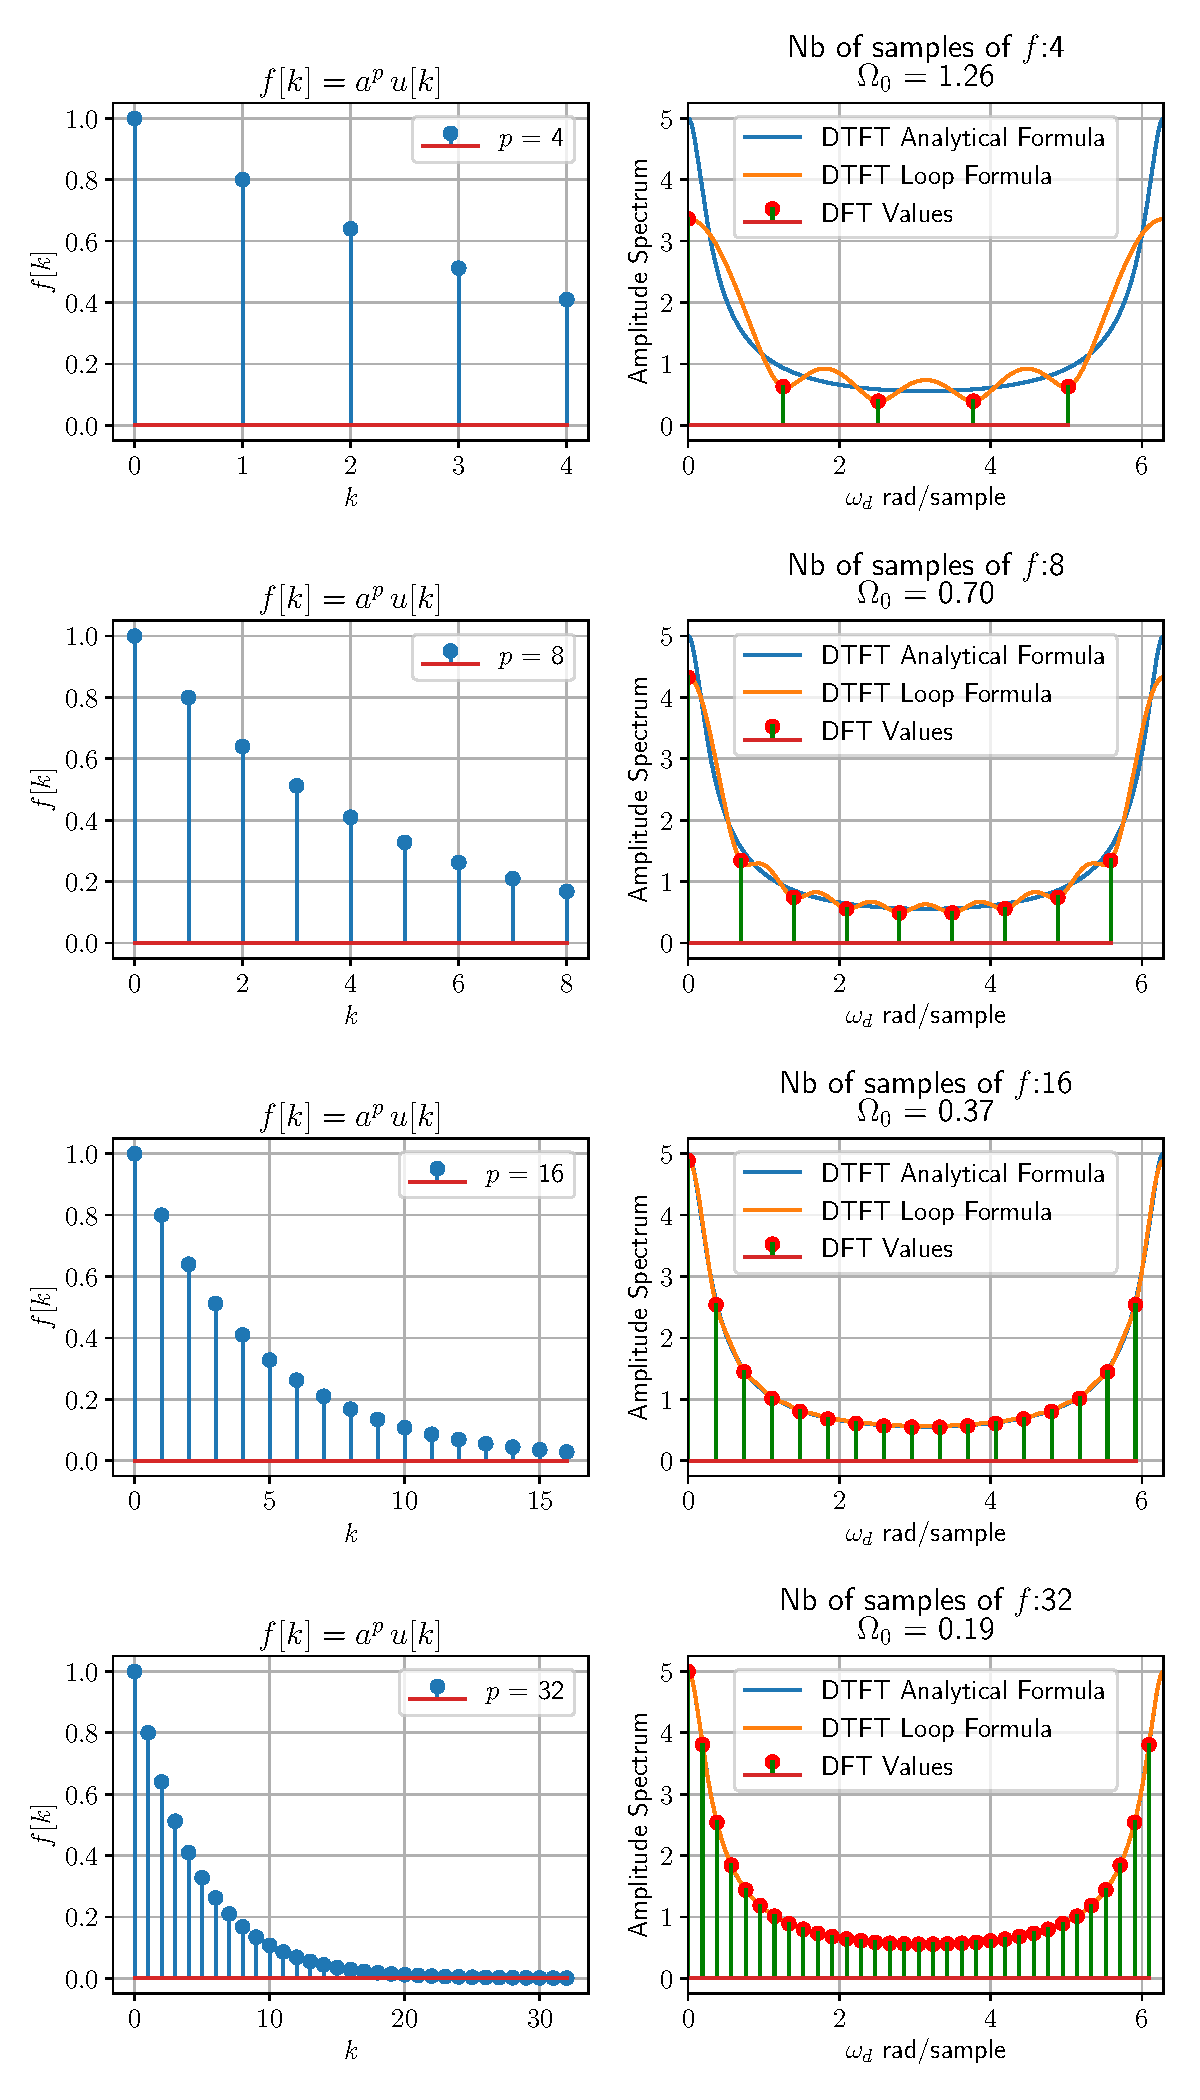
\includegraphics[width = 0.6\textwidth, frame]{Figures/DFT/DFT_Discrete_time_Infinite_Length}
\caption{Result of example of \autoref{fig:DFT:discrete_case_Infinite_length_given}}
\label{fig:DFT:discrete_case_Infinite_length_results}
\end{figure} 




\newpage

\section{Resolution and Zero Padding}

After taking all possible cases of DFT computations for continuous and discrete time signals, we do some analysis of frequency resolution using 2 sin function.

\begin{figure}[h]
\centering
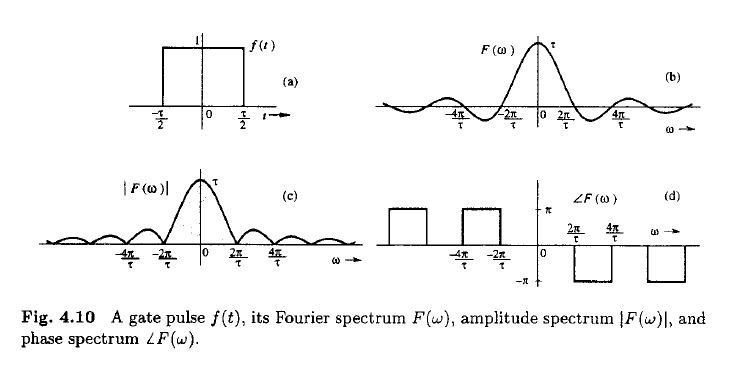
\includegraphics[width = 0.7\textwidth, frame]{Figures/DFT/rect_Fourier_transform}
\caption{rect Fourier Transform}
\label{fig:DFT:rect_Fourier_transform}
\end{figure} 

\begin{itemize}

\item Recall that $\text{sin}(\omega_0 \, t) \leftrightarrow \, j\,\pi \, \left[\, \delta(\omega_c \,- \, \omega_0) \, + \, \delta(\omega_c \,+ \, \omega_0)  \,\right]$

\item When we compute the Fourier transform of $\text{sin}(\omega_0)\, t$, the signal in theory has domain  $-\infty < \, t \, <\, + \infty$, but in reality we need to truncate the signal (or cut it), so we multiply it by a rect (pulse)

	\begin{itemize}
	\item Recall that $\text{rect} \left(\, \displaystyle\frac{t}{\tau} \,\right) \, \leftrightarrow \, \text{sinc} \left(\,\displaystyle\frac{\omega_c \, \tau}{2} \, \right)$ shown in \autoref{fig:DFT:rect_Fourier_transform}.

	\end{itemize}

\end{itemize}

Important Note about Data truncation:

\begin{itemize}

\item Let $f(t)$ some signal we want to study and $w(t)$ some window function we use where $\begin{cases}
f(t) \leftrightarrow F(\omega_c) \\
w(t) \leftrightarrow W(\omega_c) 
\end{cases}$

\item Truncation is done by multiplying the function by some window. Mathematically: 


\begin{equation}
f_w(t) \, = \, f(t) \, \times \, w(t) \leftrightarrow \, F_w(\omega_c) \, = \, F(\omega_c) \, * \, W(\omega_c)
\label{Eq:DFT:windowing_1} 
\end{equation}

	\begin{itemize}
	
	\item $f_w(t)$ denote the window signal resulting from windowing the original signal $f(t)$
	
	\item Multiplication in the time domain result in convolution in the frequency domain
	
	\item By the convolution width property, the width of the resulting signal will be the sum of the width of the 2 signal
	
	\item So as an intuition, the bandwidth of $F(\omega_c)$ will increase by the amount of the bandwidth of window function we use $W(\omega_c)$
	\end{itemize}



\item Solving equation (\ref{Eq:DFT:windowing_1}):

\begin{equation}
\begin{array}{rcl}
F_w(\omega_c) \, &=& \, F(\omega_c) \, * \, W(\omega_c) \\ \\
				 &=& \, \left(\, j\,\pi \, \left[\, \delta(\omega_c \,- \, \omega_0) \, + \, \delta(\omega_c \,+ \, \omega_0)  \,\right]   \,\right) \, * \, \text{sinc} \left(\,\displaystyle\frac{\omega_c \, \tau}{2} \, \right) \\ \\
				&=& \, \text{sinc} \left(\,\displaystyle\frac{ \tau \, \times \, (\omega_c \, - \omega_0) }{2} \, \right) \, + \, \text{sinc} \left(\,\displaystyle\frac{ \tau \, \times \, (\omega_c \, + \omega_0) }{2} \, \right) 
\end{array}
\label{Eq:DFT:windowing_2}
\end{equation}

	\begin{itemize}
	\item We have the use the property of convolution with dirac function: when convolving a function with a dirac function, the function will be shifted to the dirac location.
	\end{itemize}

\item Equation (\ref{Eq:DFT:windowing_2}) is illustrated in \autoref{fig:DFT:window_effect}

\begin{figure}[h]
\centering
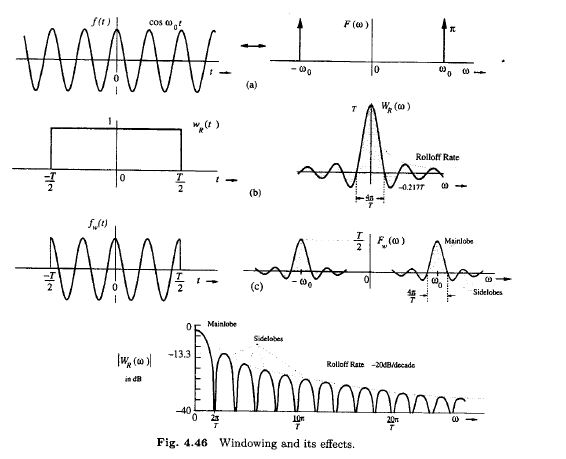
\includegraphics[width = 0.7\textwidth, frame]{Figures/DFT/window_effect}
\caption{Window effect: \tbi{spectral spreading} and \tbi{leakage}}
\label{fig:DFT:window_effect}
\end{figure} 


	\begin{itemize}
	
	
	\item The wider the window we use, the less we truncate
	
		
	\begin{itemize}
	\item Since the bandwidth of the signal is inversely proportion
	\end{itemize}
	
	
	\end{itemize}




\end{itemize}

\newpage
\subsection{1 Sinusoidal Analysis}

Consider the signal $f(t) \, = \,2 \, \text{sin} \left(\,2 \pi 500 t \,\right)$. where $F_s \, = \, 8000$ sample/s.

The study again will be by changing 2 factors: number of samples we take in the time domain (so window length) and zero padding.\\


\underline{Zero Padding Effect:}\\

We fix in this study the number of samples in the time domain (window length) and see the effect of zero padding.\\

\tbi{Rule:} zero padding doesn't effect the frequency resolution. In our case, the main lobe width will be the same whatever zero padding factor we use.

The only thing zero padding give is more sampling of the frequency spectrum, so we can get more point when plotting.

Results are shown in \autoref{fig:DFT:Spectral_Analysis_1_Sin_zero_padding}.


\begin{figure}[h]
\centering
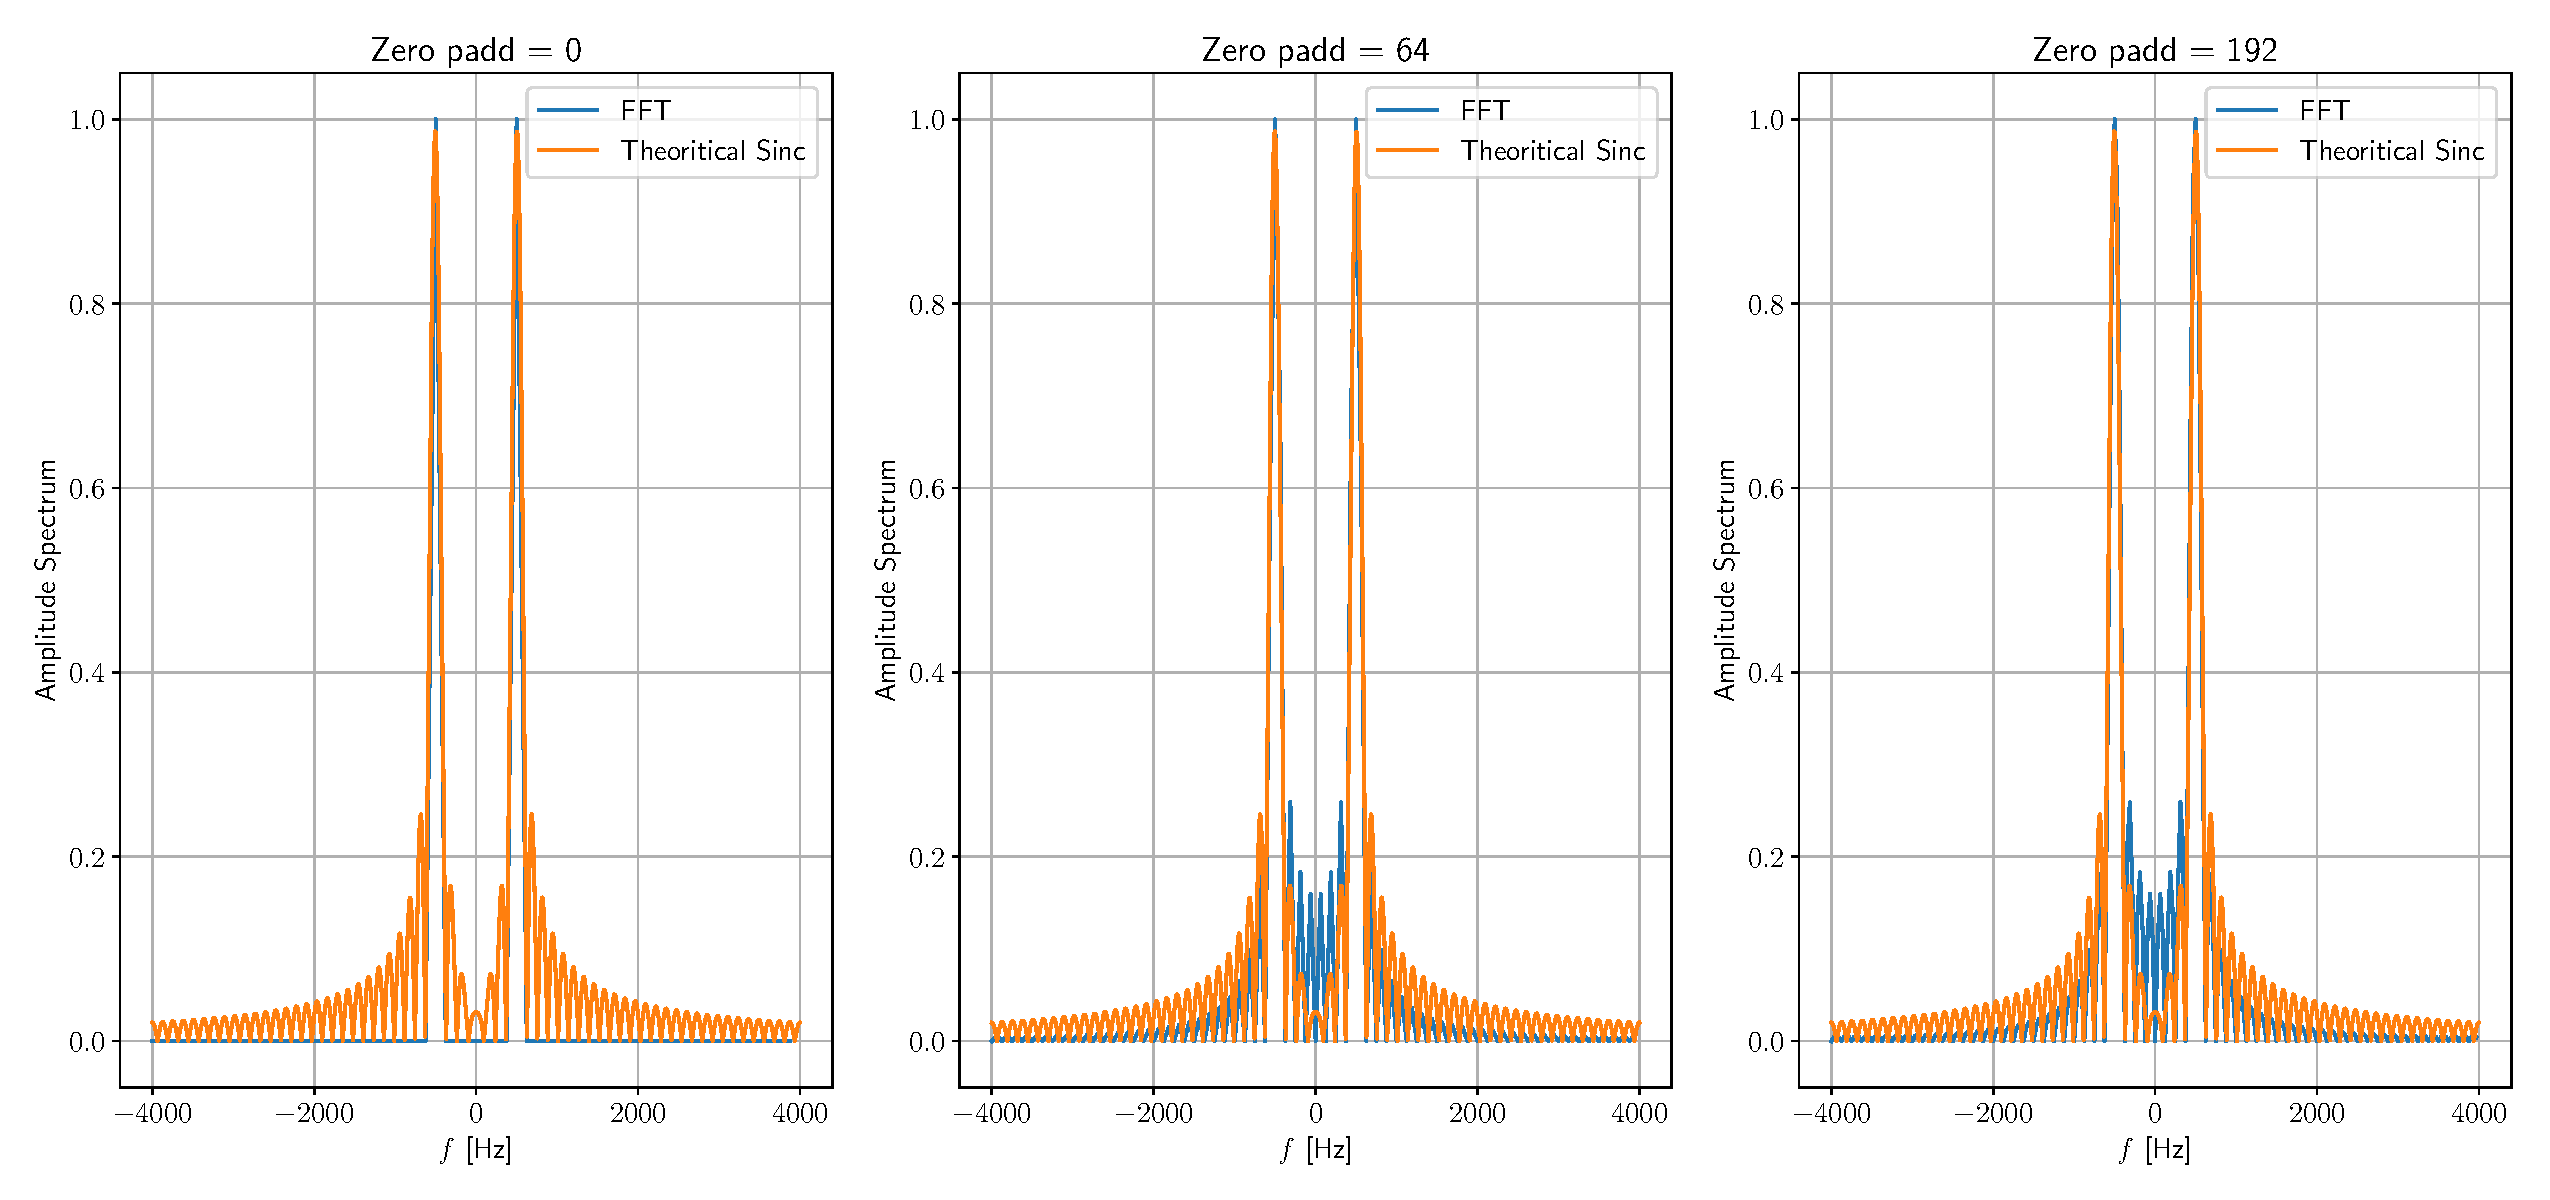
\includegraphics[width = 0.7\textwidth, frame]{Figures/DFT/Spectral_Analysis_1_Sin}
\caption{Zero Padding Effect: More samples in the frequency domain}
\label{fig:DFT:Spectral_Analysis_1_Sin_zero_padding}
\end{figure} 



%*****************************************************
%*****************************************************
%*****************************************************


\chapter{The Discrete Fourier Transform (Enhanced)}

\underline{Reference:} This way of introduction via the DTFT is from \cite{DSP_Proakis}.

\section{Introduction}

\begin{itemize}
    \item The DFT is a tool to approximate CTFT and DTFT
    
    \item First in \cite{DSP_Proakis} he talk about approximating DTFT
    
    \item Motivation for DFT:
    
        \begin{itemize}
            \item In analysing data, we always have samples and not continous time signals
            
            \item Even if we want to plug in $x[n]$ in the formula of the DTFT, we need also to evaluate on infinite grid over $[\-pi \, + \pi]$, and in computer we can't do this $\rightarrow$ this rise the need of approximation and evaluating DTFT over finite grid in $[\-pi \, + \pi]$
        \end{itemize}
    
    
    \item Be aware when using IDFT, the formula is for $N$ points, and it doesn't include zero padding option
    
        \begin{itemize}
            \item In other words, if use $M \, > \, N$ points for DFT, the IDFT use only the original $N$ points
        \end{itemize}
    
    
    \item After finishing up with the DTFT, we will see the relation between the DTFT, CTFT and DFT
    
    
    \item FFT is an algorithm to implement the DFT in an efficient manner
    
        \begin{itemize}
            \item Although people say \textit{the} FFT, but in reality there is many version of the FFT
        \end{itemize}
    
\end{itemize}


\section{Finite Duration Case}

\begin{itemize}
    \item In this section, the focus were on the understanding of the DFT for the DTFT of some finite duration signal $x[n]$
    
    
    \begin{itemize}
        \item How to take the frequency step
        
        \item How to compute the DFT Formula
        
        \item The idea of zero-padding and how it enhance the only the shape of the DFT spectrum
    \end{itemize}
    
    
\end{itemize}


\section{Infinite Duration Case}
\label{Sec:DFT:Infinite_Duration}
Now we move to the infinite duration case.

\begin{itemize}
    
\item \underline{Slide 11:}
    
        \begin{itemize}
            \item When doing this example, Prof Mark started with the case of a finite duration signal, then armed with this kind of understanding, we will tackle infinite duration case
            
            
            \item Now some person wonder: practical signal are always finite in duration, and no signal can just keep going forevever.\\
            
            Well, the infinity here may come from different cases:
            
            
            \begin{enumerate}
                \item Perhaps we are analysing some signal, which is very long and we don't have enough memory to store all (the finite) value of $x[n]$
                
                \item Maybe we are doing some radar processing, and we can't just keep waiting so long, and we need to just capture the signal and quickly analyze it (electronic warfare case)
            \end{enumerate}
            
            
        \end{itemize}
    

\item The infinite duration case can be modeled as windowing operation for the infinite duration signal 

    \begin{itemize}
        \item In frequency domain, it will be a convolution
        
        \item This will induce smearing in the DTFT spectrum of the $x[n]$
    \end{itemize}
   
   
   
\newpage    
\item So an \tbi{important point:} the DFT will help us see only the smeared spectrum of $x[n]$ as shown in \autoref{fig:DFT:what_DFT_give_us}

\begin{figure}[h]
\centering
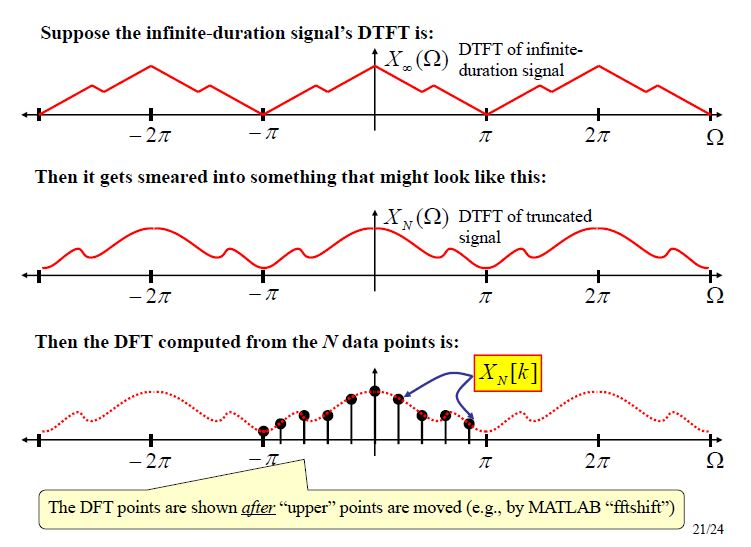
\includegraphics[width = 0.5\textwidth, frame]{Figures/DFT/what_DFT_give_us}
\caption{The DFT give us the smeared spectrum only}
\label{fig:DFT:what_DFT_give_us}
\end{figure} 



    \begin{itemize}
    
    \item The $\mathrm{2}^\mathrm{nd}$ is the smeared spectrum due to windowing 
    
    \item It is important to understand that the DFT will give us only the $\mathrm{2}^\mathrm{nd}$ row of \autoref{fig:DFT:what_DFT_give_us}
        
        \item In other words, truncation or windowing (source of error) cause a smeared spectrum (type of error)
        
        \item Another source of error is due to aliasing ( this is the $\mathrm{2}^\mathrm{nd}$ type of error we will explore its source later this later)
    \end{itemize}


    
\end{itemize}

\section{DFT for Spectral Analysis}

Now we move on for the practical use case of the DFT.

Say we have some signal we are interesting in analyzing its spectral content:

\begin{itemize}
    \item It could be a radar signal available only for a \tbi{short time}
    
    \item It could be some RF signal captured by an antenna, downcevert it and shifting it using a mixer then pass it through an ADC (or the ADC is near the antenna, and the ADC is in the bandpass mode)
\end{itemize}


\underline{\tbi{Design criteria}}: the real issue in DFT is when we reduce the samples we have for whatever the reason (signal available for only small time,$\cdots$) the resolution of the spectral component decrease.

So the big challenge is to do spectral analysis with high resolution with small amount of data.


\newpage
\subsection{Modeling the Truncation Problem}

\begin{figure}[h]
\centering
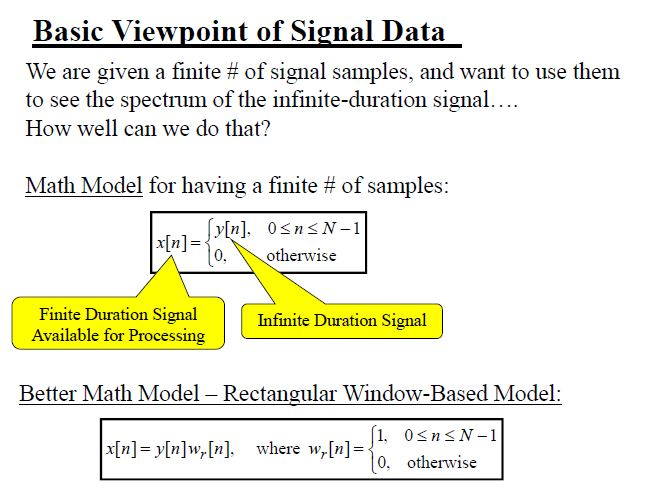
\includegraphics[width = 0.5\textwidth, frame]{Figures/DFT/truncation_modeling_1}
\caption{Truncation: using the rect window}
\label{fig:DFT:truncation_modeling_1}
\end{figure} 

\begin{itemize}
    
    \item We have some infinite signal $y[n]$ we can't collect it (recall from \autoref{Sec:DFT:Infinite_Duration} what are the other sources of infinity)
    
    \item The actual finite signal we have is $x[n]$
    
    \begin{itemize}
        \item A better mathematical modeling is the multiplication by the rect window
    \end{itemize}
    
    
    \item Be aware that in reality, all we do is collecting $N$ samples
    
    \begin{itemize}
        \item But to analyze this problem mathematically, we use the windowing idea: all the samples are given into some window and outside this window the values of these samples are 0
    \end{itemize}
    
\end{itemize}

The multiplication in time domain give us a convolution in the frequency domain, as shown in \autoref{fig:DFT:truncation_modeling_2}

\begin{figure}[h]
\centering
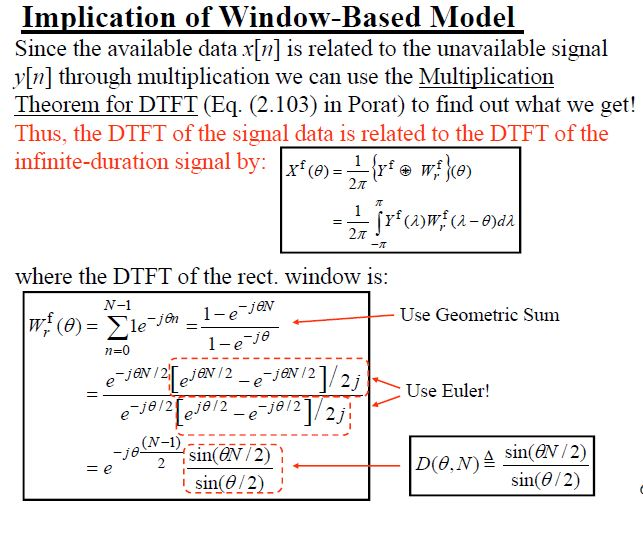
\includegraphics[width = 0.5\textwidth, frame]{Figures/DFT/truncation_modeling_2}
\caption{Truncation: using the rect window}
\label{fig:DFT:truncation_modeling_2}
\end{figure} 

\begin{itemize}
    \item The DTFT of a rect is not exactly a sinc function: it is a Drichlet function
\end{itemize}

In \autoref{fig:DFT:truncation_modeling_3}, we have the amplitude spectrum of the Drichlet for 2 values of $N$

\begin{figure}[h]
\centering
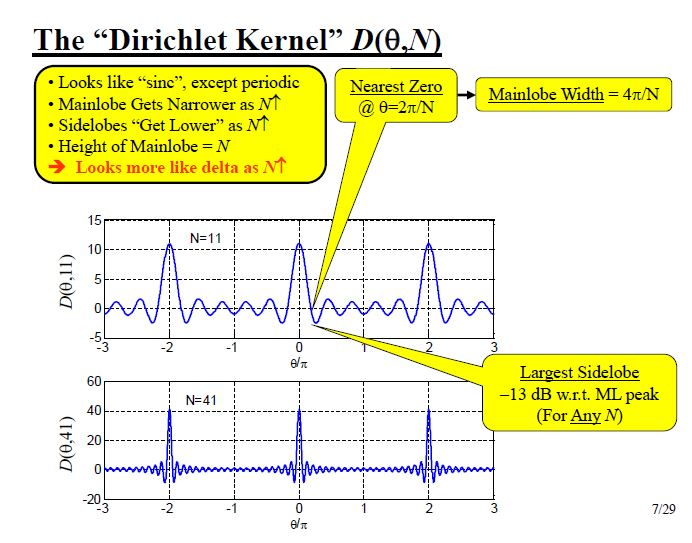
\includegraphics[width = 0.5\textwidth, frame]{Figures/DFT/truncation_modeling_3}
\caption{Truncation: using the rect window}
\label{fig:DFT:truncation_modeling_3}
\end{figure}

\begin{itemize}
    \item for a bigger $N$, 
    
    \begin{itemize}
    
        \item The mainlobe width get's smaller, converging into a delta $\leftrightarrow$ less leakage

        \item the maximum get's bigger
        
        \item But the side lobes won't get smaller 
    
    \end{itemize}
    
    
\end{itemize}


\autoref{fig:DFT:truncation_example_effect} show an example of the convolution example

\begin{figure}[h]
\centering
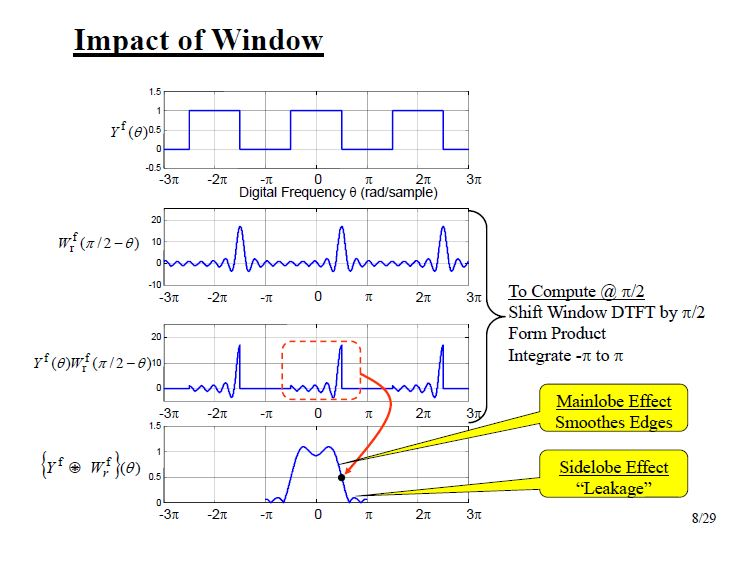
\includegraphics[width = 0.5\textwidth, frame]{Figures/DFT/truncation_example_effect}
\caption{Truncation: Exmaple}
\label{fig:DFT:truncation_example_effect}
\end{figure}

\begin{itemize}
    \item $Y(\theta)$ is the true DTFT
    
    
    \item In the $\mathrm{2}^\mathrm{row}$ we have the Drichlet shifted at $\displaystyle\frac{\pi}{2}$
    
    \item We do the multiplication and then do the intergral to obtain 1 value at the last line
    
    \item if we want to obtaine other values, we repeat the same process (sliding the window) for other values then $\displaystyle\frac{\pi}{2}$
    
    \item Notice that if the Drichlet main lobe was thinner (like a Dirac), the transition band would be sharper in the last row    
    
\end{itemize}


\section{Example}

This section take the causal exponential example, and try to simulate it to illustrate all the points we learned so far, which are summarized in \autoref{fig:DFT:Error_Types_DFT_Analysis} \\


\begin{figure}[h]
\centering
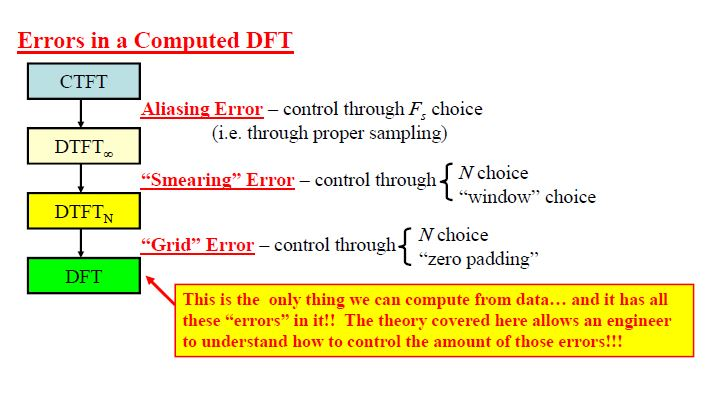
\includegraphics[width = 0.5\textwidth, frame]{Figures/DFT/Error_Types_DFT_Analysis}
\caption{Error Types in a DFT Analysis}
\label{fig:DFT:Error_Types_DFT_Analysis}
\end{figure}

Remember that in real world, all we can do is the DFT, and all the other things we can't do it since we don't necessarily have theoretical expression for the correspondent FT (CTFT or DTFT).


%******************************
%******************************
%******************************



\chapter{DFT V3}

\section{Introduction}

This chapter contains note about the DFT taken from chapter 3 in \cite{book_understanding_dsp}.


\section{Notes}

\begin{itemize}
    \item DFT Equation:
    
    
    \begin{equation}
        X[k] \, = \, \displaystyle\sum_{n \, = \, 0}^N x[n] \, \exp{\left(\, \displaystyle\frac{-j 2\pi \, n }{N} \, k \,\right)}
    \end{equation}
    
where: $\begin{cases}
k: \text{frequency index from } 0 \rightarrow N \, - \, 1 \\ 
x[n]: \text{input sequence of length }  N \\
n: \text{time domain index for the sequence } x[n]
\end{cases}$    
    
\item DFT compute the spectrum content of $N$ equally spaced frequency points    
    
\item $N$: is an important parameters since it determine 

\begin{enumerate}
    \item how much input samples are needed,
    
    \item  the resolution of the frequency domain result
    
    \item The amount of computation
\end{enumerate}
    
\item The frequency spacing: for a sampling rate $F_s$ and $N$ discrete time input sequence, the fundamental frequency in a DFT analysis is:

\begin{equation}
    \text{Fundamental Frequency} \, = \, \displaystyle\frac{F_s}{N}
    \label{Eq:DFTV3:Fundamental_Frequency}
\end{equation}

All the other frequencies will be multiple of \autoref{Eq:DFTV3:Fundamental_Frequency} $\leftrightarrow \, k \, \times \, \displaystyle\frac{F_s}{N}$.    
    
    
\newpage    
\item \underline{Leakage:}\\ 

To illustrate leakage, we give some example.

Suppose we have the following time domain signal:

\begin{equation}
x(t) \, = \, \sin{\left( \, 2 \pi 1000 \, t\,\right)} \, + \, 0.5 \, \cos{\left(\, 2 \pi 2000 \,t \, + \, \displaystyle\frac{\pi}{4}\,\right)}      
\end{equation}

If we take $N \, = \, 8$ and $F_s \, =\, 8000$ Hz, then the frequencies produced by DFT analysis (using $k \, \times \, \displaystyle\frac{F_s}{N}$):$0 \, , \, 1000\, ,\, 2000 , \, \cdots$.

Notice that the frequency bins produced by \autoref{Eq:DFTV3:Fundamental_Frequency} coincide with the  frequencies of $x(t)$. However, in real word signals we can't control usually this choice. This phenomena is what we call \tbi{leakage}.\\

Leakage can be reduced, but can't be eliminated , so we will try to understand it more.\\

The leakage problem is also treated from another starting points in different references:

\begin{itemize}
    \item For example chapter 7 in \cite{DSP_DimitrisManolakis}, they introduce the leakage through the windowing problem, and not directly manipulating the DFT equation
    
    
    \item Also they provide a good examples to illustrate what happens if the DFT bins doesn't coincide with input signal frequency
    
    
    \item The best window to use to minimize the effect of leakage and also provide a tradeoff between leakage and resolution is the Hann window
    
    
\end{itemize}

\todo{Leakage:} to do this in simulation later and \tbi{unify all these concepts}.



    
\end{itemize}








%******************************
%******************************
%******************************



\chapter{Windowing}

\underline{Source:} 

\begin{itemize}

    \item See chapter 6 in \cite{book_a_course_in_DSP_Porat}

    \item See lecture note \textit{Windows for Spectral Analysis of Signals 23} for figures and reference.
\end{itemize}



\section{Design Criteria of a Window}

\begin{itemize}

\item \underline{Slide 3}: focus on the design of window and what we need as characteristics in some particular window

\begin{itemize}
    \item Low side lobes and a rapid rate of decay
    
    \item Narrow main lobe
    
    
    \item Always a tradeoff between these 2
    
\end{itemize}


\item \underline{Slide 4}: The rectangular window has the narrowest main lobe among all the windows we will see

\begin{itemize}
    \item Side-lobe drop off rate: -6 dB/octave: octave is the double of the frequency.
    
    At each double frequency point, the side-lobe magnitude in dB decrease by 6.\\
    
    But around $\pm \pi$, the side-lobes remain constant

    
\end{itemize}

\end{itemize}


\section{Window Comparison}

\begin{itemize}

\item \underline{Slide 5-6}: Barlette Window (known also as triangular)

\begin{itemize}
    \item The idea is to lower the side-lobes level
    
    
    \item So he squared the magnitude of a rect window in frequency domain $\leftrightarrow$ convolution of 2 rect window in the time domain of size $\displaystyle\frac{N}{2}$ per window (to obtain a window of size $N$)
    
    \item As a result of this squaring, the side lobe ratio $ \left( \, \displaystyle\frac{\text{Main lobe amp}}{\text{side lobe amp}} \, \right)$ compared to a rect window has decreased
    
    
    \item Barlett has a continuity near the edge of the window (the continuity will have influence on the rate of decay of the side lobe levels)
    
    
    \item But the cost is a higher main lobe
    
\end{itemize}

\item \underline{Slide 7-8}: Hann window

\begin{itemize}
    \item He did a shifting in the frequency of rectangular window to cancell as much as he can the side lobe
    
    \item The largest side lobe level is bettet then Barlette: it is -32 dB vs -27 dB for Barlette
    
    \item And has a faster rate of decay for the side lobes compared to Barlette
    
    
\end{itemize}


\item \underline{Slide 9-10}: Hamming window

    \begin{itemize}
        \item Hamming took the idea of Hann and play on the amplitude factor
        
        \item He succeeded to obtain a lower side lobe level compared to Hann (- 43 dB compared to -32 dB for Hann)
        
        \item But the decay rate of the side lobes are much slower (6 dB/octave): this is because of the discontinuity of  the Hamming at the edge of the window
        
    \end{itemize}


\end{itemize}


\section{Derivative,Continuity and Rate of Decay}

\todo{Rate of Decay} Rate of Decay and Derivative concept: to be revisited later to see how to take derivatives as examples.

For now, I will write the main ideas

\underline{Slide 11}

\begin{itemize}
    \item In this section, we think in window in continous time to be able to use the concept of derivative
    
    \item For a rect: if we integrate we obtain a triangular function which is continuous, so $p \, = \, 0$ in this case
    
        \begin{itemize}
            \item We can't do derivative because it will give 0 
            
            \item trinagular: it will give us some function if we take the derivative, so $p \, = \, 1$
        \end{itemize}
    
    
\end{itemize}




\chapter{Discrete Time System Implementation}

\section{Introduction}

The big question in this chapter is now how to build discrete time systems.\\

We know that the output of a system at an index $k$ is done via convolution, and there is 2 types of system: FIR and IIR.

\begin{equation}
\begin{array}{rcl}
y[\, k \,] \, &=& \, \displaystyle\sum\limits_{i \, = \, 0}^{k} h[\, i\,] \, x[ \, i \, - \, k \, ] \quad \text{IIR} \\ \\
y[ \, k \,] \, &=& \, \displaystyle\sum\limits_{i \, = \, 0}^{M \, - \, 1} h[\,i \,] \, x[\, i \, - \, k \, ] \quad \text{FIR} \\ \\
\end{array}
\end{equation}


\begin{itemize}

\item Notice that in IIR, the upper limit in $\displaystyle\sum $ is the same as the index of the output signal $y$

	\begin{itemize}
	\item This is a problem, because as $k$ increase, we need to add more terms via $h[i]$
	\end{itemize}

\item However in FIR, the upper limit is constant whatever the index $k$ we need to compute for.

	\begin{itemize}
	\item Each output needs $M$ multiplication and $M \, - \, 1$ additions
	\end{itemize}

\end{itemize}

\newpage
The FIR filter can be taught as the following block diagram:

\begin{figure}[h]
\centering
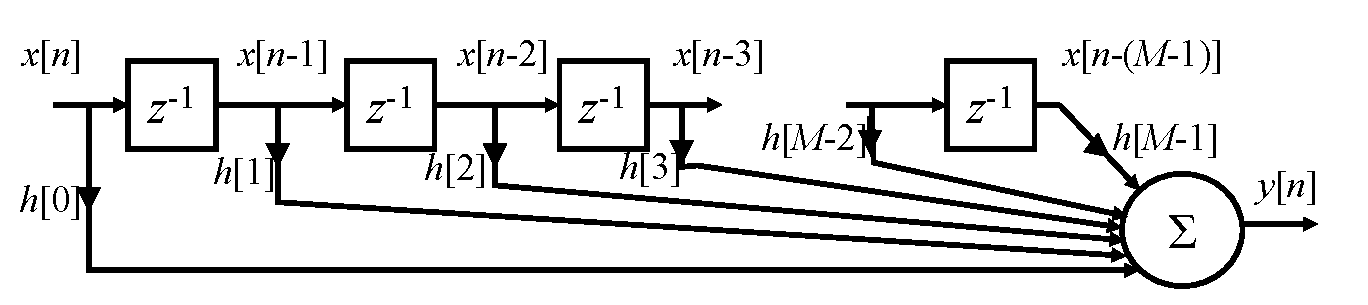
\includegraphics[width = 0.7\textwidth, frame]{Figures/discrete_time_systems/fir_block_diagram}
\caption{FIR Block Diagram}
\label{fig:discrete_time_systems:fir_block_diagram}
\end{figure} 


\begin{itemize}
\item We are assuming causal signal $x[n]$ and system $h[n]$

\item For each clock cycle, so for each value of index $n$:

	\begin{itemize}
	\item $y[0] \, = \, x[0] \, h[0]$, and all the other terms are 0 since we are causal system/signal
	
	\item In the next clock cycle $y[1]$: $x[0]$ gets shifted (the term $x[n \, - \, 1]$), and hence for $n \, = \, 1$ 
	
	
\begin{equation}
\begin{array}{rcl}
y[1] \, &=& \, x[n] \, h[0] \, + \, x[n \, - \, 1] \, + \, h[1] \\ \\
		 &=& x[1] \, h[0] \, + \, x[1 \, - \, 1] \,  h[1] \\ \\
		 &=& x[1] \, h[0] \, + \, x[0] \,  h[1] \, + \, \cdots
\end{array}
\end{equation}	
	
and all the other terms are 0

	\end{itemize}

\end{itemize}


The FIR block diagram shown in is called \tbi{feeforward} because everything is coming in forward direction to the $\displaystyle\sum$ block.


\section{IIR and Recursion}


Theoretically, convolution can implement FIR and IIR, but in IIR it poses problem regarding computation.\\

In this section, we see how we can implement \tbi{some} IIR system using recursion (feedback).\\

Consider the accumulator system:

\begin{equation}
y[n] \, = \, \displaystyle\sum\limits_{i \, = \, 0}^n x[i]
\label{Eq:discrete_time_systems:accumulator}
\end{equation}

which is an IIR system having an impulse response $h[n] \, = \, u[n]$. We can rewrite \autoref{Eq:discrete_time_systems:accumulator} as:

\begin{equation}
\begin{array}{rcl}
y[n] \, &=& \, \displaystyle\sum\limits_{i \, = \, 0}^n x[i] \\ \\		
		&=& \, \displaystyle\sum\limits_{i \, = \, 0}^{n \, - \, 1} x[i] + \, x[n] \\ \\
		&=& \, y[n \, - \, 1] \, + \, x[n]
\end{array}
\label{Eq:discrete_time_systems:accumulator_2}
\end{equation}

So to compute the current output sample $y[n]$, we need to save a value of the past output sample $ y[n \, - \, 1] $ and add the current input sample $x[n]$.\\

\autoref{Eq:discrete_time_systems:accumulator_2} lead to the concept of general $N^{\text{th}}$ order linear constant coefficient difference equation:

\begin{equation}
y[n] \, + \, a_1 \, y[n \, - \, 1] \, + \, \cdots \, + a_N \, y[n \, - \, N] \, = \, x[n] \, + \, b_1 \, x[n \, - \, 1] \, + \, \cdots \, + b_M \, y[n \, - \, M]
\label{Eq:discrete_time_systems:difference_eq}	
\end{equation}

\autoref{Eq:discrete_time_systems:difference_eq} can be rewritten in recursive form:

\begin{equation}
y[n] \, = \, - \, \displaystyle\sum\limits_{k \, = \, 1}^N a_k \, y[n \, - \, k] \, + \, \displaystyle\sum\limits_{k \, = \, 0}^M b_k \, x[n \, - \, k]
\label{Eq:discrete_time_systems:difference_eq_recursive} 
\end{equation}

\autoref{Eq:discrete_time_systems:difference_eq_recursive} can be used to compute the current output sample $y[n]$ using a finite amount of resources.


\section{Block Diagrams}

Block diagrams are the first step in implementing discrete time systems. They help us to define the internal structure of a discrete time systems, so they can help us when writing code or thinking about a specific hardware to implement and deploy discrete time systems.\\

We first begin from a specific example, and then take the results to generalize them.

\newpage
\subsection{First Order Difference Equation and Direct Form} 

Suppose we want to construct the block diagram of the following $\mathrm{1}^\mathrm{st}$ order difference equation:

\begin{equation}
y[n] \, = \, - \, a_1 \, y[n \, - \, 1] \, + \, b_0 \, x[n] \, + \, b_1 \, x[n \, - \, 1]
\label{Eq:discrete_time_systems:first_oder_difference_eq}
\end{equation}

\begin{itemize}

\item It is called $\mathrm{1}^\mathrm{st}$ order because the output samples $y[n]$ and $y[n \,  - \, 1]$ differ only by 1 sample

\item There are 2 delays: from input and output.

\end{itemize}

A straightforward block diagram of \autoref{Eq:discrete_time_systems:first_oder_difference_eq} is shown in 
\autoref{fig:discrete_time_systems:direct_form_1_first_order_diff_eq}.


\begin{figure}[h]
\centering
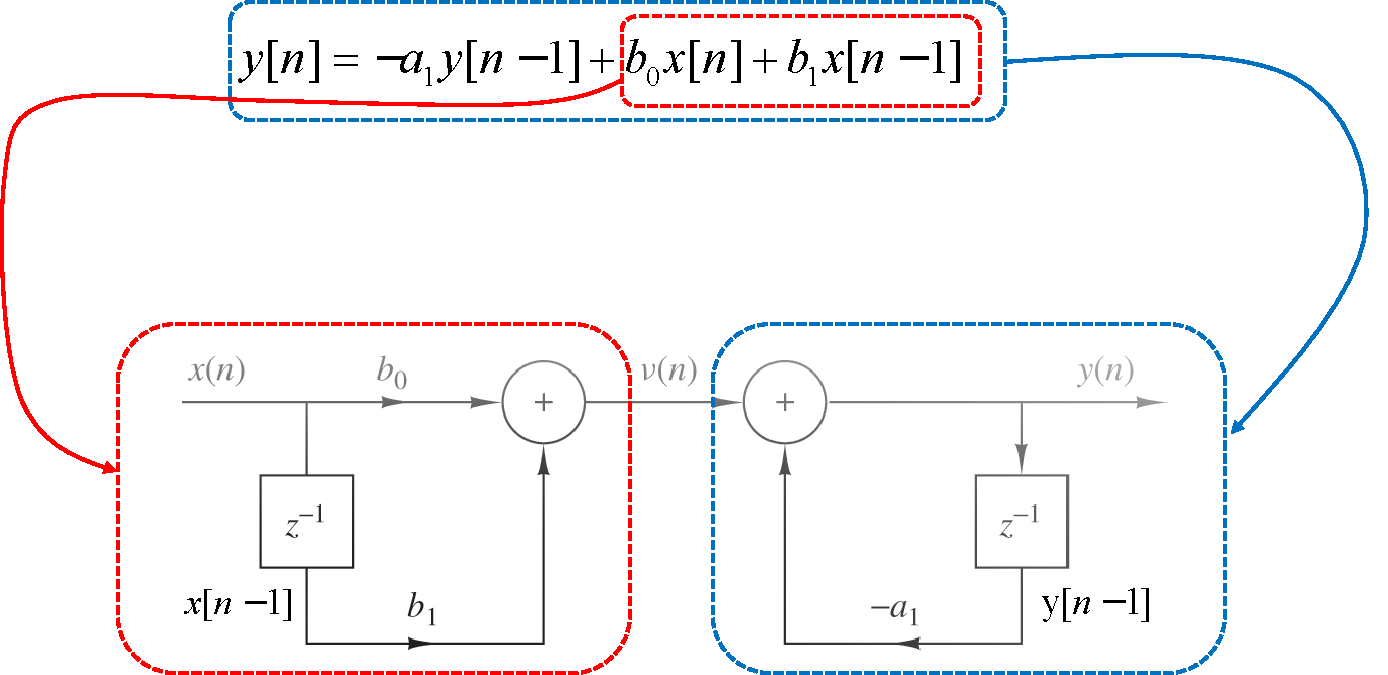
\includegraphics[width = 0.7\textwidth, frame]{Figures/discrete_time_systems/direct_form_1_first_order_diff_eq}
\caption{Direct Form I for $\mathrm{1}^\mathrm{st}$ order difference equation}
\label{fig:discrete_time_systems:direct_form_1_first_order_diff_eq}
\end{figure} 

\begin{itemize}

\item It is called \tbi{direct form I} because the delays of input and output are separated

\end{itemize}

Remember that delays elements are storage units (memory units) which holds previous samples, so the less we have memory the less resources we need.\\

\newpage
We can reduce delays elements by doing a handy trick: since we are working in LTI systems, we can \tbi{interchange the order of the systems without affecting the results}. Theses steps are shown in \autoref{fig:discrete_time_systems:interchange_order}.


\begin{figure}[h]
\centering
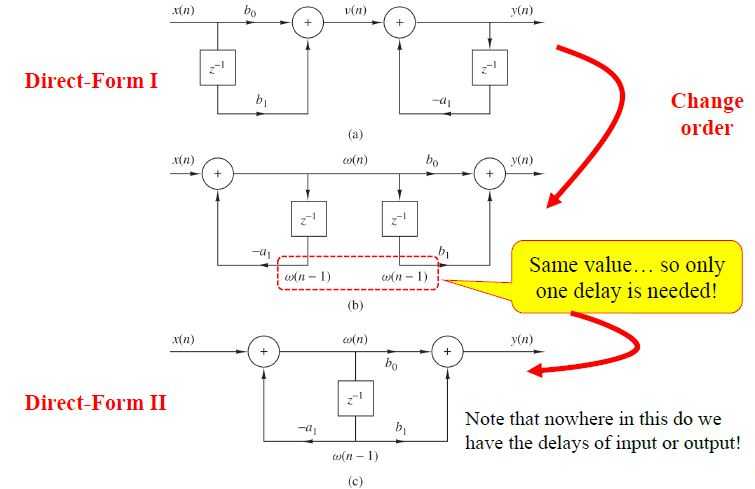
\includegraphics[width = 0.7\textwidth, frame]{Figures/discrete_time_systems/interchange_oder}
\caption{Interchanging order to reduce delay elements}
\label{fig:discrete_time_systems:interchange_order}
\end{figure} 

\begin{itemize}

\item Notice that in b), we have the same \tbi{intermediate number} $\omega(n)$ as input to the same delays, that's why we need 1 delay element only and not 2

\end{itemize}

Final results is shown in \autoref{fig:discrete_time_systems:direct_form_2_first_order}.

\begin{figure}[h]
\centering
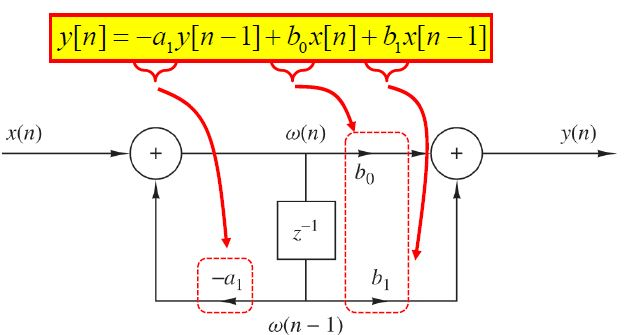
\includegraphics[width = 0.7\textwidth, frame]{Figures/discrete_time_systems/direct_form_2_first_order}
\caption{Direct form II for $\mathrm{1}^\mathrm{st}$ order difference equation}
\label{fig:discrete_time_systems:direct_form_2_first_order}
\end{figure}

\newpage
\subsection{General Direct Form}

Now we can generalize the direct form 1 and 2 from previous sections.


\begin{figure}[h]
\centering
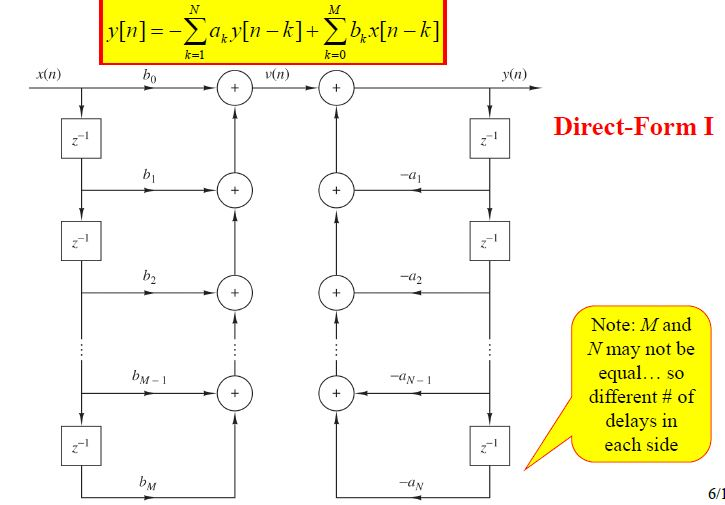
\includegraphics[width = 0.5\textwidth, frame]{Figures/discrete_time_systems/direct_form_1_general}
\caption{Direct form I General Form}
\label{fig:discrete_time_systems:direct_form_1_general}
\end{figure}

\begin{figure}[h]
\centering
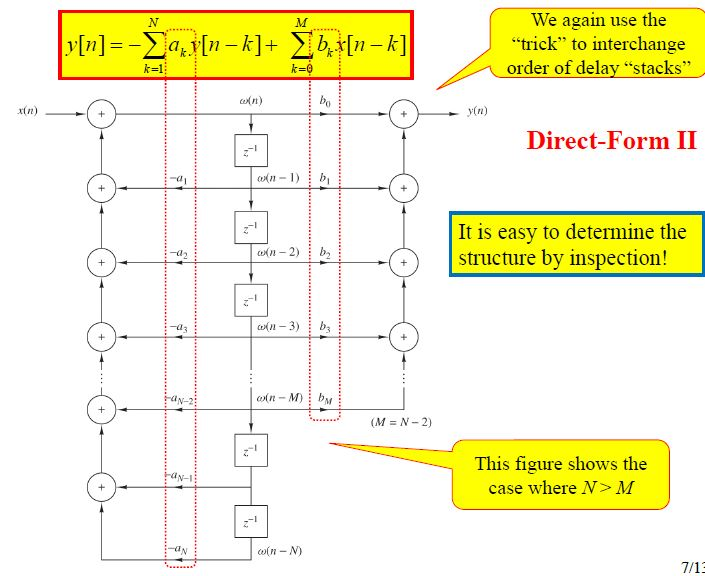
\includegraphics[width = 0.5\textwidth, frame]{Figures/discrete_time_systems/direct_form_2_general}
\caption{Direct form II General Form}
\label{fig:discrete_time_systems:direct_form_2_general}
\end{figure}

\begin{itemize}

\item Note that it is not necessary that $N \, = \, M$, so we can have different delay elements in direct form 1

\item For direct form 2: if $N \, \neq \, M$, we don't take branches always

\end{itemize}


\subsection{Recursion and Non Recursion}

Direct form 2 constitute from 2 parts: the $b_k$ (input coefficients), which are directly fed into the sum blocks, so they are \tbi{non-recursive}

\section{General Filter Design Concept}

Before diving into specific design technique for FIR or IIR, we present some general concept concerning filters in generals.

\begin{enumerate}

\item Discrete time filters present much more advantage over analog filters since we can use digital signal processing


\item Ideal response of a filter can't be achievable since the impulse response is a non-causal (sinc function)


\item We can only implement causal system

	\begin{itemize}
	\item Causal system are proven by Proney-Wiener Theorem, which give us a causal $h[n]$ for square integrable and convergent ln integral
	
		
		\item But also since we want the integral of the ln to converge, we can't allow for $H_{\text{filter}}(\omega_d)$ to take 0 on some interval, or the integral will blow up since ln 0 tends to $+\infty$, but we can have 0 values for some points $\leftrightarrow$ we can't have perfect stop band
				
	\end{itemize}


\item Structure of the Filter:

Proney-Wiener Theorem just says that mathematically we can obtain a causal response $h[n]$, but it doesn't state anything about the structure of the filter.\\

Our goal in filter design is to approximate some desired frequency response $H_{\text{desired}}$ using a rational transfer function.

	\begin{itemize}
	\item Why rational ? because using rational transfer function, we can implement filter using conventional block diagrams
	\end{itemize}

\item Practical Specifications: Every filter type have characteristics when designing: pass band, transition band, and ripples shown in 

\begin{figure}[h]
\centering
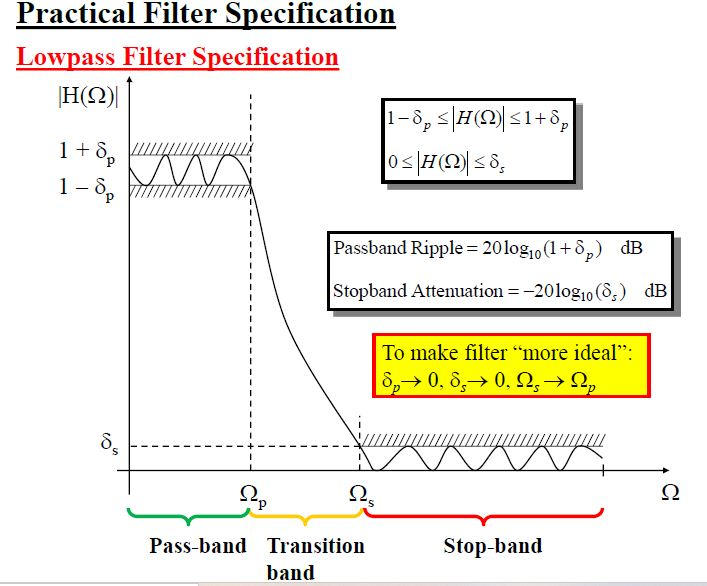
\includegraphics[width = 0.5\textwidth, frame]{Figures/discrete_time_systems/filter_specs}
\caption{Practical Filter Specification}
\label{fig:discrete_time_systems:filter_specs}
\end{figure}


	\begin{itemize}
	\item The more we approach ideal filter case $\leftrightarrow \, \delta_p \rightarrow \, 0 , \, \delta_s \rightarrow \, 0 $ and $\Omega_s \, \rightarrow \, \Omega_p$ (narrower transition band), the more the designing of the filter (IIR or FIR) become more complex
	
	
	\item Concerning the stop band attenuation: it is $ -20 \text{log}_10 \delta_s $, we put a - to make it positive because when we say attenuation, we say for example attenuation of 40 dB, but in reality it is -40 dB	
	
	\end{itemize}


\item FIR and IIR comparison: To do later.

	

\end{enumerate}



\chapter{FIR Design}

\section{Linear Phase Revisited}

Before diving into the design of FIR filters, we revise the concept of linear phase because it will be used later.\\

If we have some transfer function $H(\omega_d)$, it is called linear phase if the angle spectrum has the form of a straight line.\\

The linear phase is caused because the amplitude spectrum of $H(\omega_d)$ pass through 0, which causes a flip in the angles, as shown in \autoref{fig:FIR:linear_phase_example}.


\begin{figure}[h]
\centering
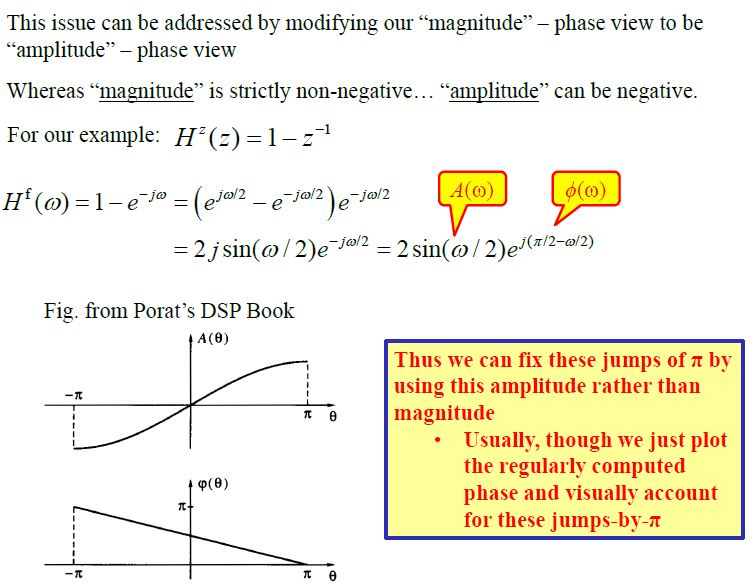
\includegraphics[width = 0.5\textwidth, frame]{Figures/FIR/linear_phase_example}
\caption{An example of linear phase system function}
\label{fig:FIR:linear_phase_example}
\end{figure}

\begin{itemize}

\item Notice that we let the amplitude $A(\omega_d)$ be positive and negative

    \begin{itemize}
        \item Not like MATLAB command \verb|abs| which compute the amplitude spectrum only using positive values
    \end{itemize}

\end{itemize}

In numerical computation using MATLAB, the angle spectrum will be shift by $\pi$, because MATLAB won't allow angle values be bigger then $\pi$.\\

An example is shown in \autoref{fig:FIR:linear_phase_example_matlab}, where every time the angle will be bigger then $\pm \pi$, MATLAB will do a shift by $2 \pi$, and this cause to make the jumps in the plots.\\

\begin{figure}[h]
\centering
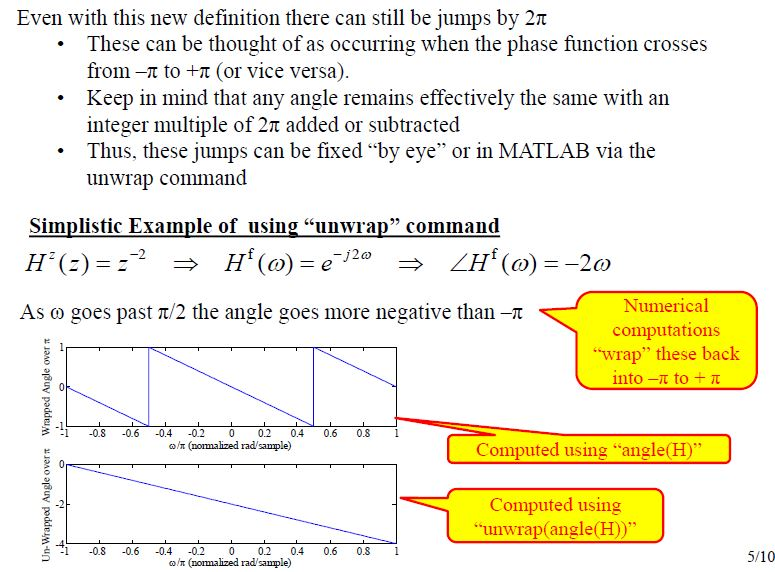
\includegraphics[width = 0.5\textwidth, frame]{Figures/FIR/linear_phase_example_matlab}
\caption{Wrapping Error for Phase Spectrum}
\label{fig:FIR:linear_phase_example_matlab}
\end{figure}

To fix the $2 \pi$ jumps, we can use the \verb|unwrap| command. But be aware, that \verb|unwrap| \tbi{fix only $ \pm 2 \pi$ jumps, and not the $ \pm \pi$ jumps}.
Notice for example that $\omega \, = \, 0$, $\phi(\omega) \, \neq \, 0$, and this is due to $\pi$ shift.\\

Handling $\pi$ shift is done theoretically or by hand.

\section{Linear Phase for FIR}

\subsection{Recap for FIR Equations}

\begin{figure}[h]
\centering
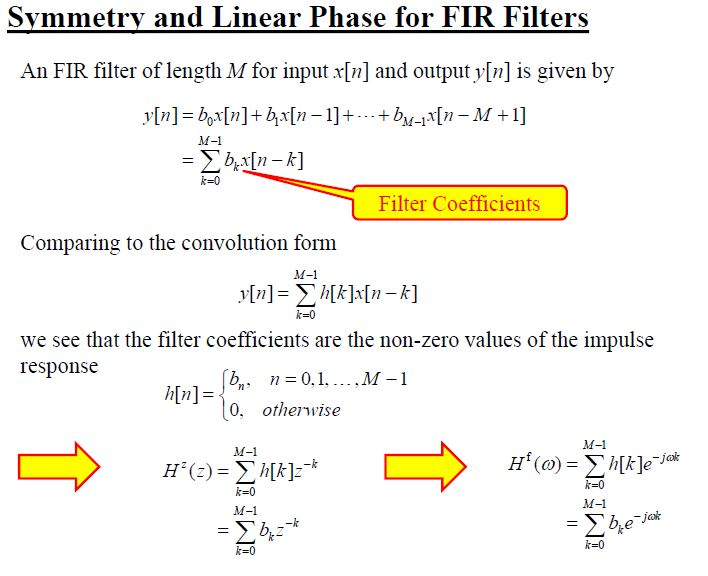
\includegraphics[width = 0.5\textwidth, frame]{Figures/FIR/FIR_Recap}
\caption{FIR Recap}
\label{fig:FIR:FIR_Recap}
\end{figure}

\begin{itemize}
    \item We have the difference equation of an FIR filter
    
    \item The impulse response $h[n]$ is composed from coefficients of the difference equation
    
    
    \item Filter coefficients are called \tbi{taps}
    
    
\end{itemize}


\subsection{Linear Phase definition for FIR}

We say that an FIR is linear in phase if its impulse response has symmetry

\begin{equation}
    h[k] \, = \, \pm \, h[M \, - \, 1 \, - \, k] \quad \text{for } k \, = \, 0 \, , \, 1 \, , \, \cdots \, , \, M \, - \, 1
\label{Eq:FIR:FIR_Symmetry_Impulse_Response}
\end{equation}

\begin{figure}[h]
\centering
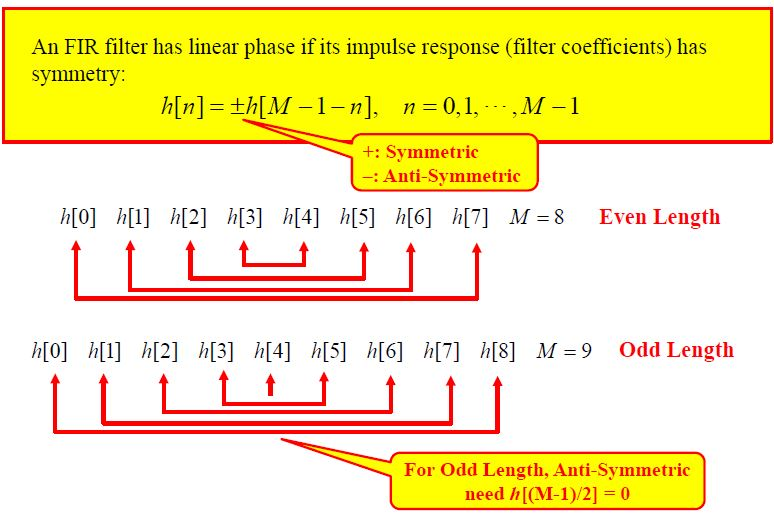
\includegraphics[width = 0.5\textwidth, frame]{Figures/FIR/FIR_Symmetry}
\caption{FIR Symmetry}
\label{fig:FIR:FIR_Symmetry}
\end{figure}

Notice that for odd length, we have a constraint for antisymmetric case. In the example of \autoref{fig:FIR:FIR_Symmetry}, if we have in symmetric case, we can say that $h[4] \, = \, h[4]$. But if we are in antisymmetric case, the only way we can say that $h[4] \, = \, -\,h[4]$ is if $h[4] \, = \, 0$, so we have some constraint to keep in mind in case of odd length antisymmetric case.\\

Using \autoref{Eq:FIR:FIR_Symmetry_Impulse_Response}, it can be shown that the frequency response $H_{\text{FIR}}(\omega_d)$ can be written in the form of an amplitude times an exponential having a linear phase. For a specific case demonstration, an example is shown in \autoref{fig:FIR:FIR_Symmetry_Proof_Example}, where the proof is done for the case of symmetric even length.

\begin{figure}[h]
\centering
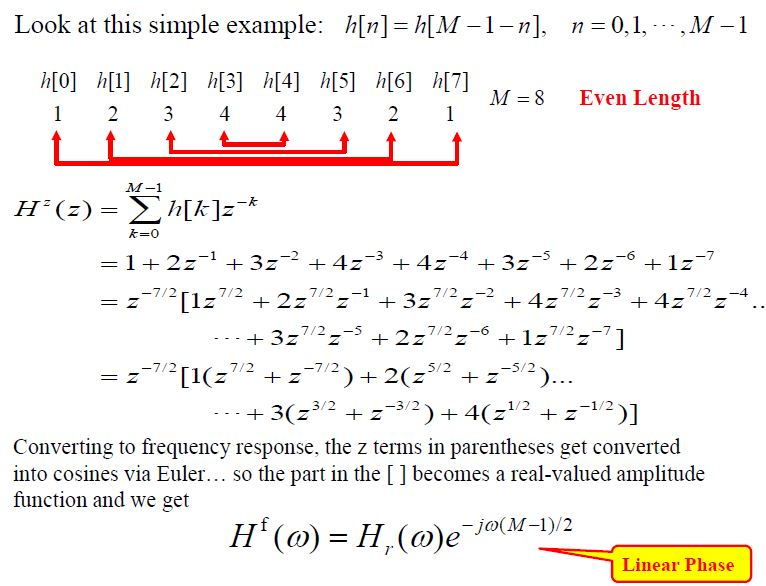
\includegraphics[width = 0.5\textwidth, frame]{Figures/FIR/FIR_Symmetry_Proof_Example}
\caption{FIR Linear Phase Proof by a example}
\label{fig:FIR:FIR_Symmetry_Proof_Example}
\end{figure}

\underline{General Formula:}\\


\begin{equation}
\begin{array}{rcl}
h[M \, - \, 1 \, - \, k] \, &=& \, \rightarrow \,  H_{\text{FIR}}(\omega_d) \, = \, \text{Amp}(\omega_d) \, \exp \left( \,  \displaystyle\frac{-j \, \omega_d \, (M \, - \, 1)}{2}  \,\right)  \\ \\
- \, h[M \, - \, 1 \, - \, k] \, &=& \, \rightarrow \,  H_{\text{FIR}}(\omega_d) \, = \, \text{Amp}(\omega_d) \, \exp \left( \,  \displaystyle\frac{-j \, \omega_d \, (M \, - \, 1)}{2}  \, + \, \displaystyle\frac{\pi}{2} \right)  \\ \\
\end{array}    
\end{equation}

For antisymmetric case, we have a shift of $ \displaystyle\frac{\pi}{2} $ in the phase spectrum.

\subsection{Zero Pattern}

For a linear phase FIR filter, we get an inverse of zero in addition to the initial one.

\subsection{Use case for Symmetric and Anti-symmetric}

Antisymmetric are note suited for LPF, because $H( \omega_d \, =\, 0) \, = \, 0$, which is not wanted in a LPF frequency response.

\section{Window Design Technique}

This method is not the commonly used one since it is not that effective, but it is a simple one and a good starting point.\\

In \autoref{fig:FIR:FIR_LPF_Sinc}, we have some LPF with some cut-off frequency to design. The impulse response is a sinc which is non-causal. The phase is linear.\\


\begin{figure}[h]
\centering
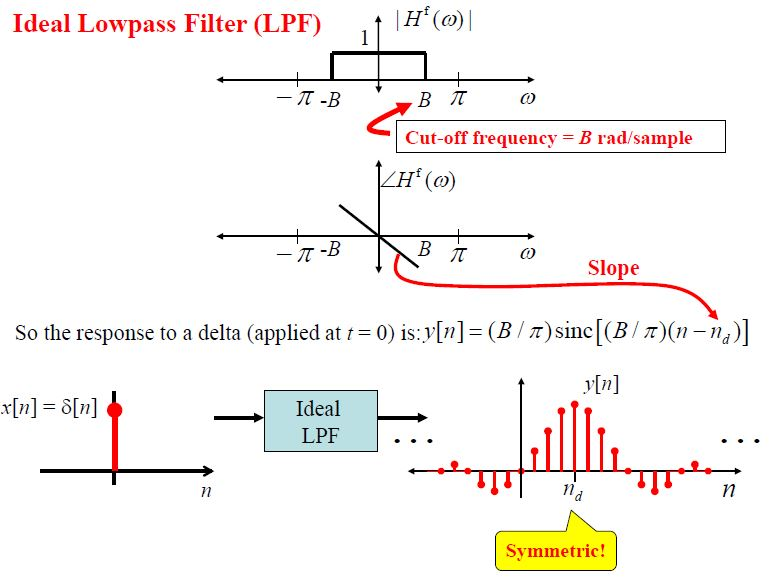
\includegraphics[width = 0.5\textwidth, frame]{Figures/FIR/FIR_LPF_Sinc}
\caption{LPF FIR}
\label{fig:FIR:FIR_LPF_Sinc}
\end{figure}

\underline{Design Key:} Usually we are interested that the phase is linear, but we don't care that much with its slope. We see later how we can achieve certain slope.\\

\newpage
The best way to make it causal is to simply truncate the values before 0, and also we truncate the symmetrical part which are after 0 to preserve the symmetry. The filter response after truncation is shown in \autoref{fig:FIR:FIR_window_method_truncation}.

\begin{figure}[h]
\centering
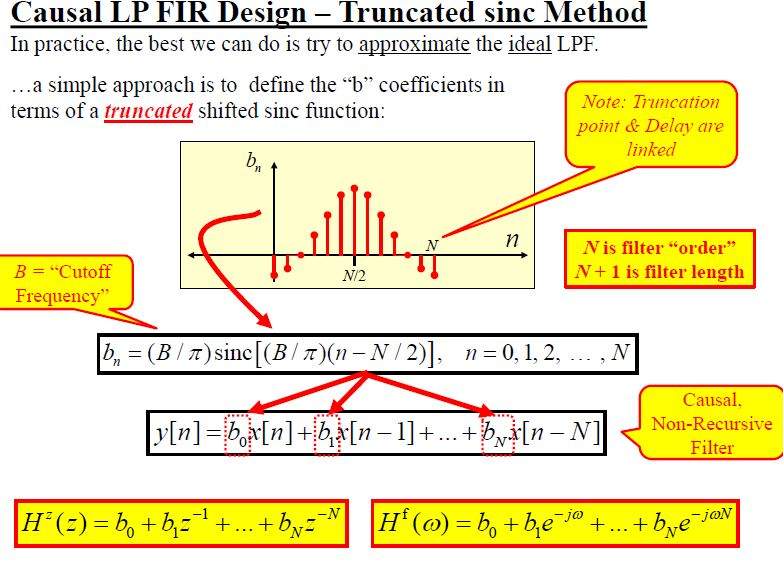
\includegraphics[width = 0.5\textwidth, frame]{Figures/FIR/FIR_window_method_truncation}
\caption{Truncation Method}
\label{fig:FIR:FIR_window_method_truncation}
\end{figure}

In this type of design to obtain a integer shift, we have to choose $N$ even.\\

An example is shown in \autoref{fig:FIR:FIR_window_method_example}.

\begin{figure}[h]
\centering
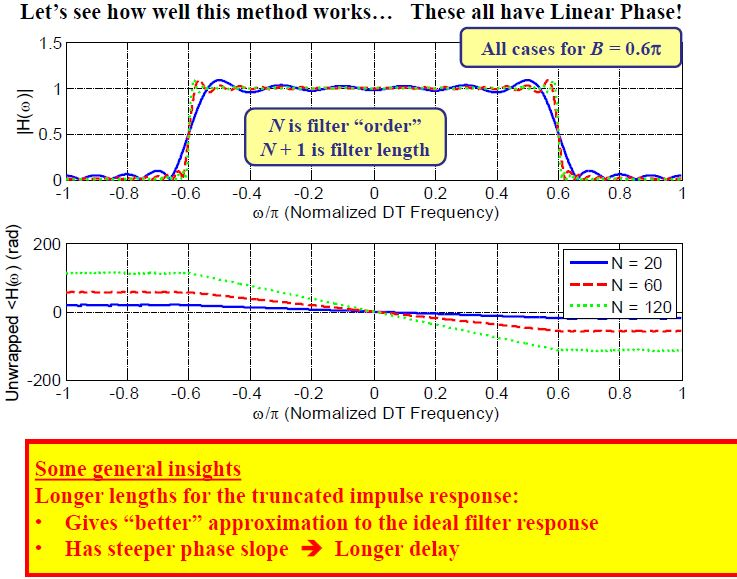
\includegraphics[width = 0.5\textwidth, frame]{Figures/FIR/FIR_window_method_example}
\caption{Truncation Method}
\label{fig:FIR:FIR_window_method_example}
\end{figure}


\begin{itemize}
    \item Notice that when the order $N$ increase, we have a more sharper transition bandwidth.
        
        \begin{itemize}
            \item This is true for any desing, and not only this particular desing
        \end{itemize}
    
    \item The downside of this is that we don't get to enhance the ripples at the edge of the pass band even when we increase the order
    
\end{itemize}

\newpage
Another example in dB scale is shown \autoref{fig:FIR:FIR_window_method_example_dB}.

\begin{figure}[h]
\centering
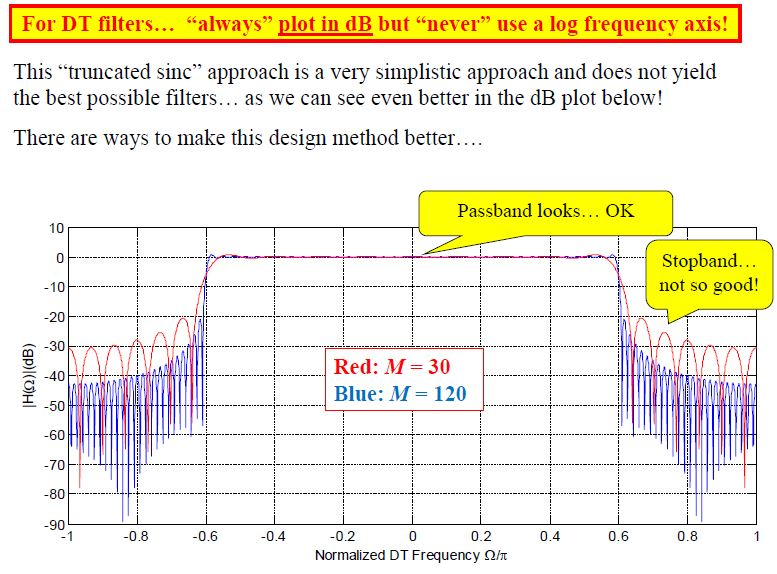
\includegraphics[width = 0.5\textwidth, frame]{Figures/FIR/FIR_window_method_example_dB}
\caption{Example of design in dB scale: stop band is not good at all}
\label{fig:FIR:FIR_window_method_example_dB}
\end{figure}

Even with the increase of the order, we have no a big difference the stop band attenuation levels between $M \, = \,30$ and $M \, = \, 120$.\\

\subsection{The usage of other window}

The problem of truncation is can simply formulated by multiplying the desired impulse response by some window, and hence we can use the knowledge of window types and tradeoff to controll the characteristic of the desired filter specification.

The lack of performance in the stop band seen in \autoref{fig:FIR:FIR_window_method_example_dB} is due to the sidelobes of rectangular window, which don't get lower even when we increase the length (hence the order of the filter).

Recall from Window analysis we have:

\begin{itemize}
    
\item Windows usually cause \tbi{smearing}

\item Usually we want some $h_{\text{desired}}[k]$, but we have is some windowed impulse due to windowing

\item Mathematically:
\begin{equation}
\begin{array}{rcl}
     h[k] \, &=& \, h_{\text{desired}}[k \, - \, k_d] \, \times \, w[k]  \\ \\
     H(\omega_d) \, &=& \, \displaystyle\frac{1}{2 \, \pi} \displaystyle\int\limits_{- \pi}^{+\pi} H_{\text{desired}}(\omega_d) \, W(\omega_d \, - \, \omega_0) \, d\omega_d
\end{array}    
\end{equation}

\item The sidelobes of the rectangular window will affect the ripples: the pass band (at the edge) and the stop band height

\item Whereas the mainlobe will controll the transition bandwidth of the filter

\end{itemize}


So as a design criteria:

\begin{itemize}
    \item Choose the window shape to get side lobes we want
    
    
    \item The length of the window control the transition band
    
\end{itemize}


\section{Frequency Sampling Technique}

The frequency sampling method rely on DFT computation, and taking finite frequency points at multiple of $\displaystyle\frac{2 \pi}{M}$. The steps are shown in \autoref{fig:FIR:FIR_frequency_sampling_method}


\begin{figure}[h]
\centering
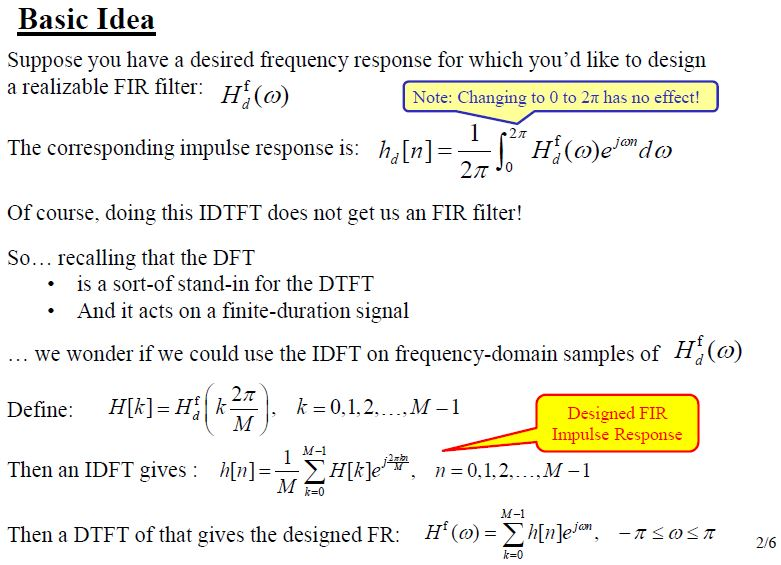
\includegraphics[width = 0.5\textwidth, frame]{Figures/FIR/FIR_frequency_sampling_method}
\caption{FIR using frequency sampling method}
\label{fig:FIR:FIR_frequency_sampling_method}
\end{figure}

\begin{itemize}
    

\item The period of integration in computing $h_{\text{desired}}[n]$ is changed to $0 \rightarrow \, 2 \pi$ instead of $- \pi \rightarrow +\pi$, in order to cover the frequency indices $k$ when computing the frequency response of the desired filter $H_{\text{des}}[k]$ at fininte frequency indices

\item Then we apply the inverse DFT to get some finite time domain signal which represent the desired filter (causal and finite)

\item As a check, we apply the DTFT again to the computed impulse response to check the filter


\end{itemize}

Summary results are shown in \autoref{fig:FIR:FIR_frequency_sampling_results}.

\begin{figure}[h]
\centering
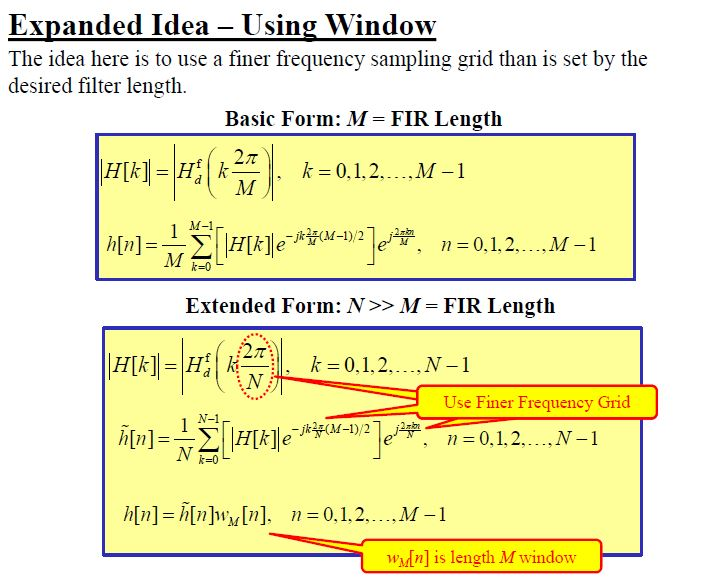
\includegraphics[width = 0.5\textwidth, frame]{Figures/FIR/FIR_frequency_sampling_results}
\caption{FIR using frequency sampling results}
\label{fig:FIR:FIR_frequency_sampling_results}
\end{figure}

\begin{itemize}

\item Usually we have $|H[k]|$ are specified

\item To ensure a linear phase, we add the term $e^{-j \, k \, \frac{2 \pi}{M} \, \left( \, \frac{M \, - \, 1}{2} \, \right) }$

\item The term $e^{j \, \frac{2 \pi k \, n}{M}}$ is from  the inverse DFT process

\item To enhance the design, more frequency sampling points $N >> \, M$ are taken

    \begin{itemize}
        \item But this give us a filter bigger then the desired
        
        \item That's why we multiply the $h_d[n]$ by a window
    \end{itemize}

\end{itemize}

Illustration using MATLAB shown in \autoref{fig:FIR:FIR_frequency_sampling_matlab}

\begin{figure}[h]
\centering
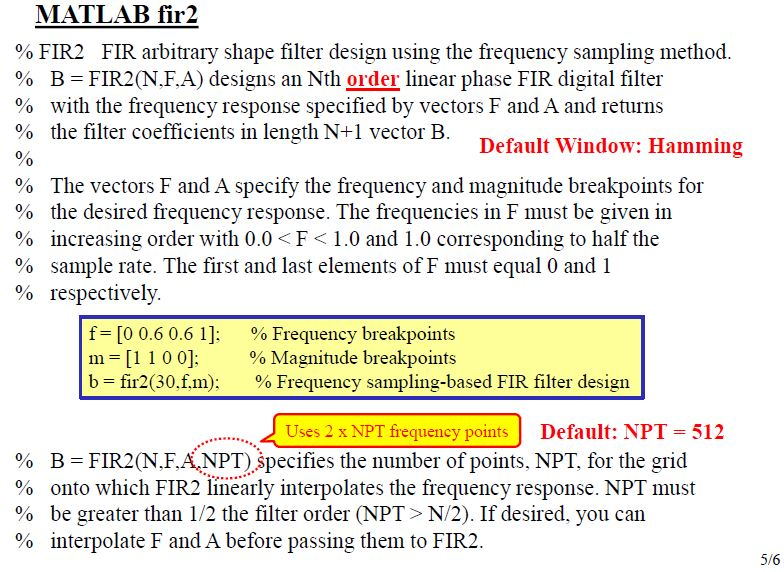
\includegraphics[width = 0.5\textwidth, frame]{Figures/FIR/FIR_frequency_sampling_matlab}
\caption{FIR using frequency sampling results}
\label{fig:FIR:FIR_frequency_sampling_matlab}
\end{figure}


\begin{itemize}
    \item $N$ is the order
    
    \item By default, number of frequency points is $2 \, \times \, 512$
    
    \item \verb|fir2| can make arbitrary (some special effect) in some frequency bands, unlike \verb|fir1|
    
    \item \verb|f| is inputed as a normalized vector in units of $\pi$, and \verb|m| is the desired magnitude
    
        \begin{itemize}
            \item In the example of \autoref{fig:FIR:FIR_frequency_sampling_matlab}, from $0 \rightarrow -0.6$, we have our passband since \verb|m| is 1 in this region
        \end{itemize}
    
\end{itemize}

\newpage
\section{Optimum Equiripple}

\begin{figure}[h]
\centering
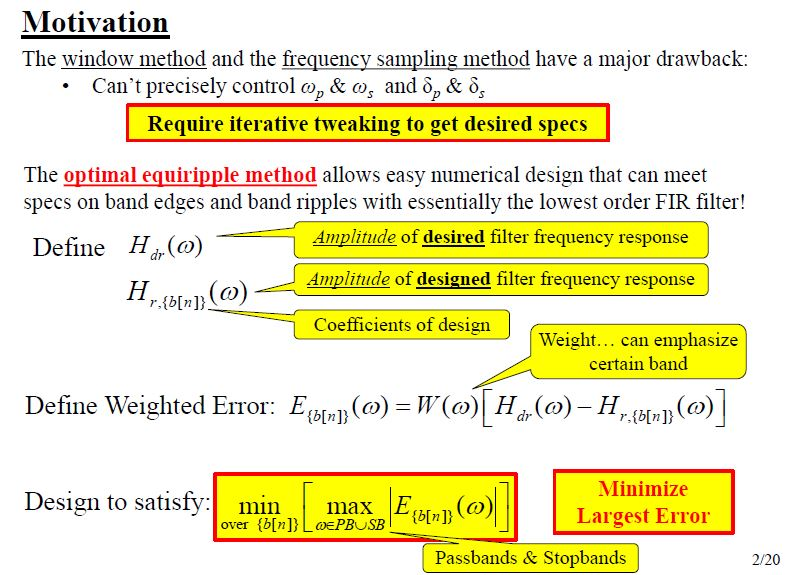
\includegraphics[width = 0.5\textwidth, frame]{Figures/FIR/FIR_optimum_equiripple}
\caption{FIR using Optimum Equiripple Method}
\label{fig:FIR:FIR_optimum_equiripple}
\end{figure}

\begin{itemize}

\item It was proposed by Parcs and McCellan in 1972, and implemented in FORTRAN

\item Drawback of previous designed methods: need to keep iterating to get the specs of the filter, and even after finishing iterating we won't get them all

\item The design criteria: minimize the largest error between the desired filter and the designed filter

    \begin{itemize}
        \item $H_{r \, , \, b[n]}$: in the designed filter, we explicitly show the coefficient $b[n]$ because there will be used using the design process
        
        \item $\max_{\omega \in PB \cup SB}$: maximize over all the pass band and the stop band $\leftrightarrow$ we don't care what happen in the transition band
        
    \end{itemize}


\end{itemize}

\subsection{MATLAB Example}


\begin{figure}[h]
\centering
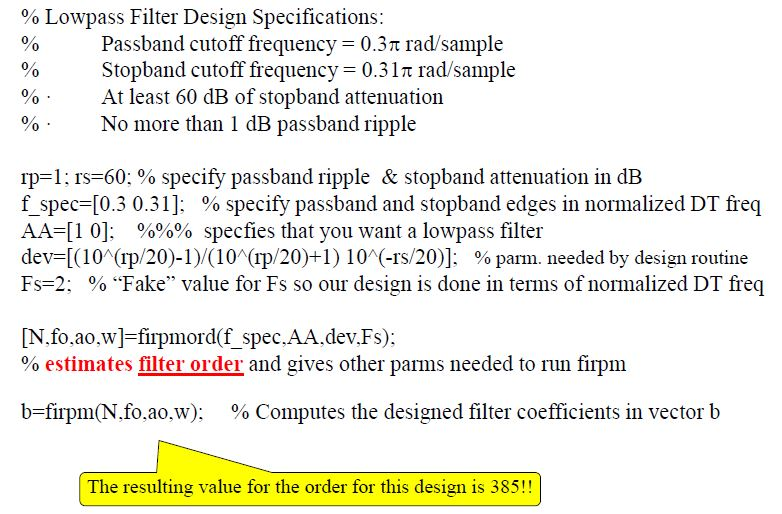
\includegraphics[width = 0.5\textwidth, frame]{Figures/FIR/FIR_optimum_equiripple_matlab_example}
\caption{FIR using Optimum Equiripple: A MATLAB Example}
\label{fig:FIR:FIR_optimum_equiripple_matlab_example}
\end{figure}


\begin{itemize}

\item First we are specifying the ripples in the pass band and the stop band $\leftrightarrow$ \verb|rp| and  \verb|rs|

\item Then we set the cuttoff frequencies \tbi{without the $\pi$} (the range goes from $0 \rightarrow 1$), this how MATLAB expects the frequencies

\item The sampling rate $F_s \, = \, 2$: we choose this value because usually we expect the range of frequencies from $0 \rightarrow \displaystyle\frac{F_s}{2}$.\\

If $F_s \, = \, 2 \rightarrow \,\displaystyle\frac{F_s}{2} \, = \, 1$, which corresponds to the range of the actual frequencies

    \begin{itemize}
        \item If we want to desing some pyhsical frequencies in Hz, we need to know the actual sampling rate in hz also.\\
        
        As an example: \verb|f-spec = [pass = 1000 , stop = 5000 Hz]| and $F_s \, = \, 40$KHz
    \end{itemize}

\item The \verb|dev| parameters is for the ripples $\delta_p$ and $\delta_s$: we convert them into linear scale

    \begin{itemize}
        \item Notice the - singe in front of \verb|rs| in the \verb|dev| variable: this is because it is an attenuation
    \end{itemize}


\end{itemize}

\subsection{Revisiting the Optimum Equiripple}

\todo{FIR Design}: To redo this section later.\\

In a broad view (this is from Dr Barry Veen), the optimum equiripple design consists of:

\begin{itemize}
    \item An objective function: a minimax criterion, where minimize over the coefficient of the FIR filter, the max absolute error between the desired (ideal) and the designed (actual)
    
    \item Take for example 1 form of the linear phase FIR (all of the contains cos terms)
    
    \item Use Chebychev polynomial (approximation theory), alternation theorem for the error, then Remez exchange algorithm, all of these methods are grouped under the name Parks-McCellan algorithm, which have used these mathematical tools to form fast, flexible FIR design method
    
    \item Unlike the previous 2 methods (window method and frequency sampling), the ripples in the pass and stop band were the same, but in some application we may have some different tolerance.
    
    The equiripple method can give us different tolerance, but in the expense of having equiripple oscillations (so not perfectly flat as before in window method and frequency sampling)
    
    
\end{itemize}




\chapter{IIR Filter}

\section{Introduction}

\begin{figure}[h]
\centering
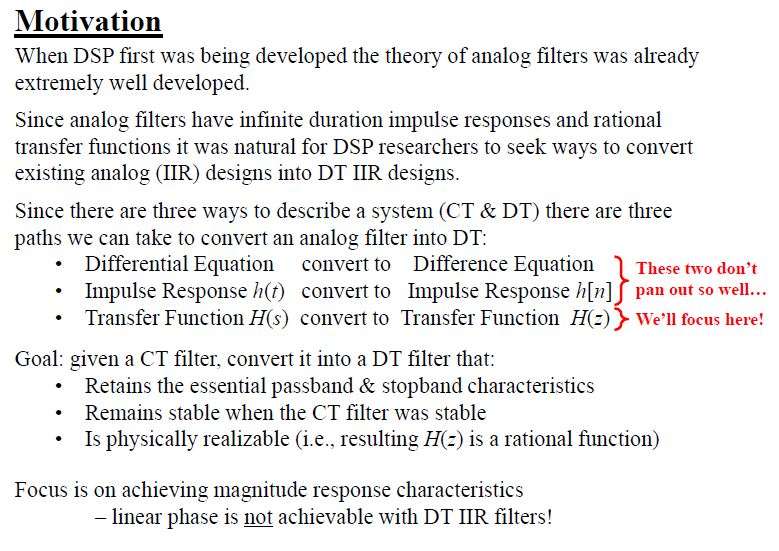
\includegraphics[width = 0.7\textwidth, frame]{Figures/IIR/Introduction}
\caption{IIR Design principle}
\label{fig:IIR:Introduction}
\end{figure}


DSP research started early in 1960 and 1970. Back then, all analog filter were implemented using analog components (resistor,inductor,capacitor,$\cdots$). What the DSP researchers hope to do is to implement these same analog filter using discrete time approach.\\


A system can be represented using 3 components: differential equation,transfer function and impulse response. What we will do is try to convert each one of them into its discrete time equivalent , and then apply the design.\\


The first 2 elements (differential equation,impulse response) don't work that much in designing IIR, so we will focus on them briefly and focus on transfer function element.

\newpage
\section{Notation}

Since we are dealing with transfer functions, and moving from analog to discrete time and frequency, we will have allot of notation illustrated in \autoref{fig:IIR:Notation_Convention}.

\begin{figure}[h]
\centering
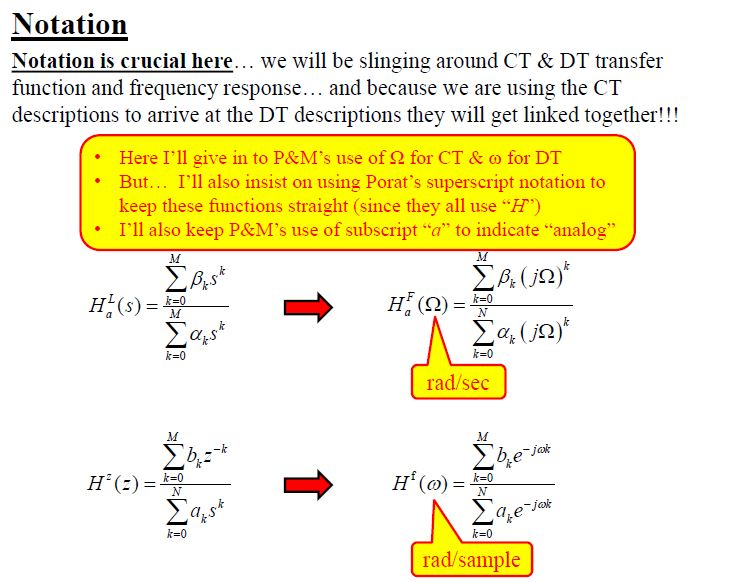
\includegraphics[width = 0.7\textwidth, frame]{Figures/IIR/Notation_Convention}
\caption{Notation Convention}
\label{fig:IIR:Notation_Convention}
\end{figure}


\newpage
\section{Difference Equation Approach}


In difference equation: we take some differential equation which represent the behaviour of some analog filter, turn it into a difference equation, then apply $z$-transforms for example to derive $H(z)$.\\

The conversion from differential equation $\rightarrow$ difference equation is done using approximation of derivative as shown in \autoref{fig:IIR:difference_eq_change_of_variables}

\begin{figure}[h]
\centering
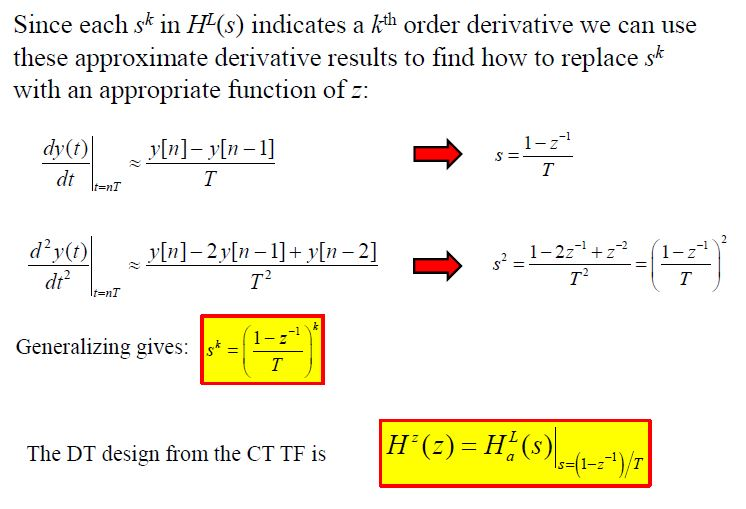
\includegraphics[width = 0.7\textwidth, frame]{Figures/IIR/difference_eq_change_of_variables}
\caption{Difference equation approach: using derivative approximation to make a change of variable from $s \rightarrow z$}
\label{fig:IIR:difference_eq_change_of_variables}
\end{figure}


Inverting the relation $s \, = \, \displaystyle\frac{1 \,  - \, z^{-1}}{T_s}$ give us $z \, = \, \displaystyle\frac{1}{1 \, - \, s \, T_s}$. Illustration using $s$-plane and $z$-plane is shown in \autoref{fig:IIR:difference_eq_change_of_variables_2}

\begin{figure}[h]
\centering
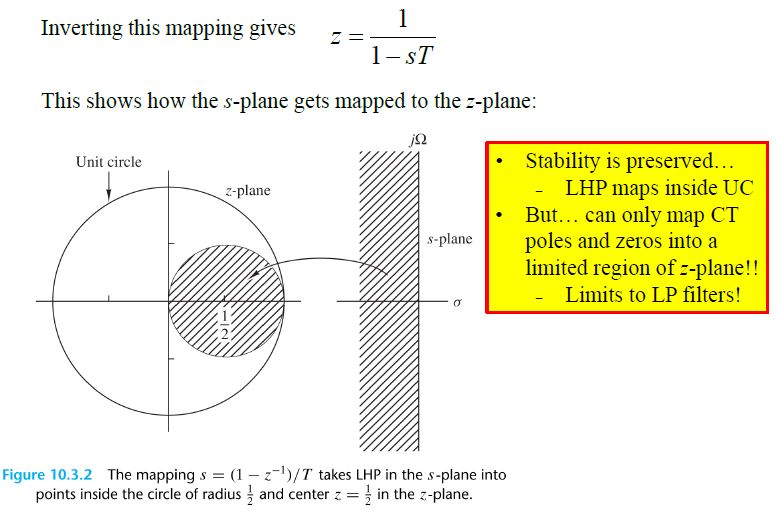
\includegraphics[width = 0.7\textwidth, frame]{Figures/IIR/difference_eq_change_of_variables_2}
\caption{Difference equation  $s \rightarrow z$ mapping using complex planes}
\label{fig:IIR:difference_eq_change_of_variables_2}
\end{figure}

Notice that in \autoref{fig:IIR:difference_eq_change_of_variables_2}, we don't have all the stable $z$-plane. So in filter design implication, we are only limited to LPF.

\section{Impulse Invariance Approach}

It takes the impulse function in the \textit{continuous frequency domain}, and turn into a \textit{discrete frequency domain} as shown in \autoref{fig:IIR:impulse_invariance}.

\begin{figure}[h]
\centering
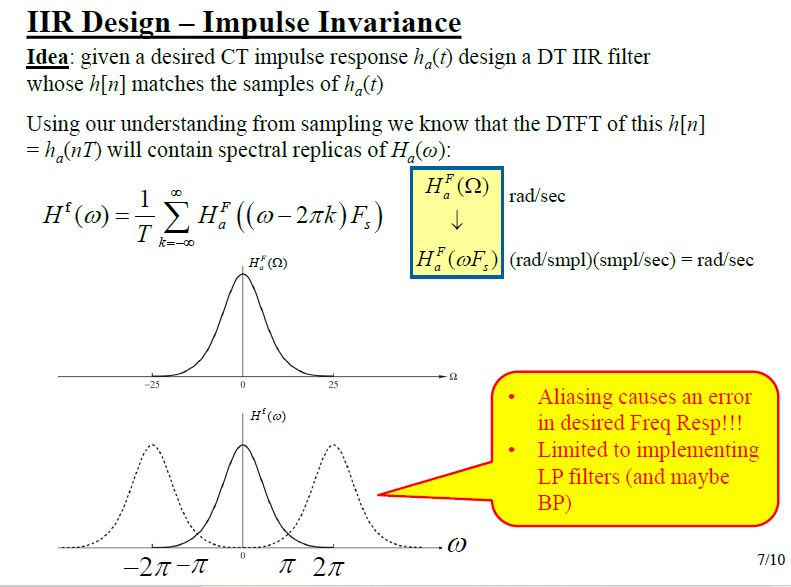
\includegraphics[width = 0.7\textwidth, frame]{Figures/IIR/impulse_invariance}
\caption{Impulse Invariance Approach: Sampling the continuous transfer function}
\label{fig:IIR:impulse_invariance}
\end{figure}

Nevertheless, in \autoref{fig:IIR:impulse_invariance} it is not very clear how to use this fact to build some discrete time system and convert it to rational transfer function. This is illustrated in \autoref{fig:IIR:impulse_invariance_2}.


\begin{figure}[h]
\centering
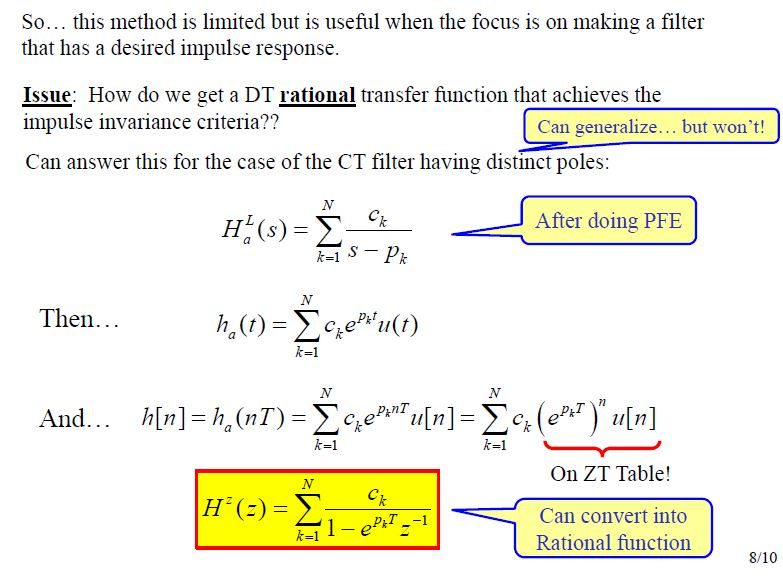
\includegraphics[width = 0.6\textwidth, frame]{Figures/IIR/impulse_invariance_2}
\caption{Impulse Invariance Approach: converting to a rational transfer function}
\label{fig:IIR:impulse_invariance_2}
\end{figure}


\newpage
\subsection{Example}

An example is shown in \autoref{fig:IIR:impulse_invariance_example}.

\begin{figure}[h]
\centering
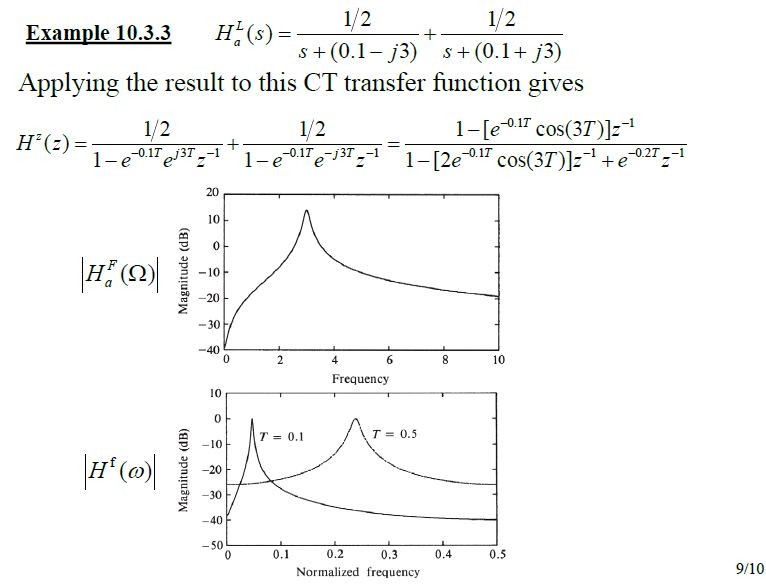
\includegraphics[width = 0.7\textwidth, frame]{Figures/IIR/impulse_invariance_example}
\caption{Impulse Invariance Approach Example}
\label{fig:IIR:impulse_invariance_example}
\end{figure}

For a bigger $T_s$, we get shift in the resonance frequency.

\newpage
\section{Bilinear Transformation}

\underline{Note:} here the term \textit{transformation} doesn't mean as in the context of Fourier or Laplace transform, but it means in the context of mapping. But this name has stuck in it in the history.\\

As a first step, what we have done before is the usage of transfer function concept. This is illustrated in \autoref{fig:IIR:bilinear_intro}.


\begin{figure}[h]
\centering
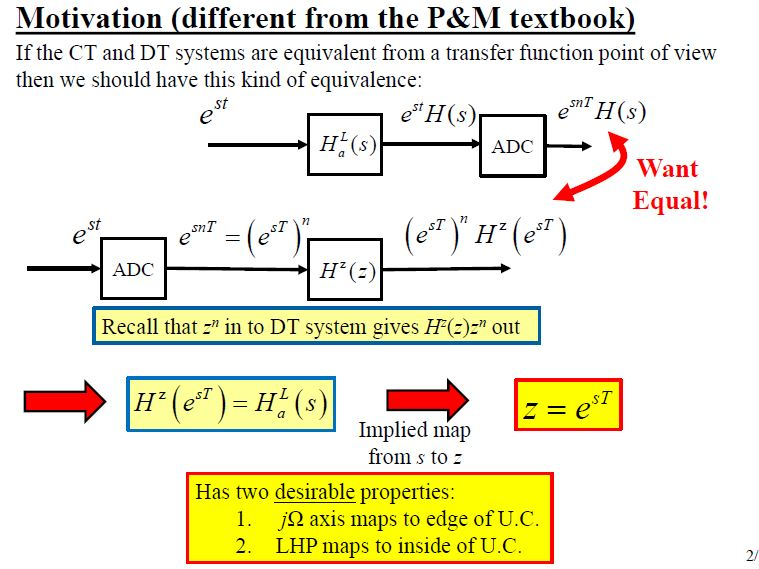
\includegraphics[width = 0.7\textwidth, frame]{Figures/IIR/bilinear_intro}
\caption{Using Transfer function concept}
\label{fig:IIR:bilinear_intro}
\end{figure}

If we want to compare, we need to use and ADC in the front end (as shown in the $\mathrm{2}^\mathrm{nd}$ row of \autoref{fig:IIR:bilinear_intro}). This lead to derive the $\mathrm{1}^\mathrm{st}$ mapping relation:

\begin{equation}
    z \, = \, e^{s\, T}
    \label{Eq:IIR:1st_mapping}
\end{equation}

\autoref{Eq:IIR:1st_mapping} have some nice properties, like stability (left half plain mapped into the uniform circle of $z-$plane). However, it causes some wrapping (which is similar to aliasing), as shown in \autoref{fig:IIR:wraping}.


\newpage
\begin{figure}[h]
\centering
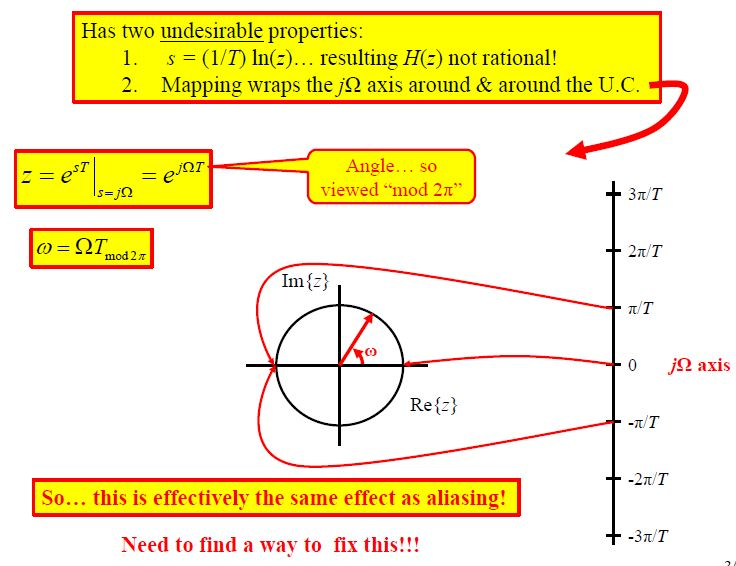
\includegraphics[width = 0.7\textwidth, frame]{Figures/IIR/wraping}
\caption{Using Transfer function concept}
\label{fig:IIR:wraping}
\end{figure}

In order to solve this problem, we need to modify the mapping. The final result will be:

\begin{equation}
    s \, = \, \left( \, \displaystyle\frac{2}{T} \, \right) \, \displaystyle\frac{z \, - \, 1}{z \, + \, 1}
    \label{Eq:IIR:2nd_mapping}
\end{equation}

\newpage
The proof of \label{Eq:IIR:2nd_mapping} is shown in \autoref{fig:IIR:proof_mapping}.

\begin{figure}[h]
\centering
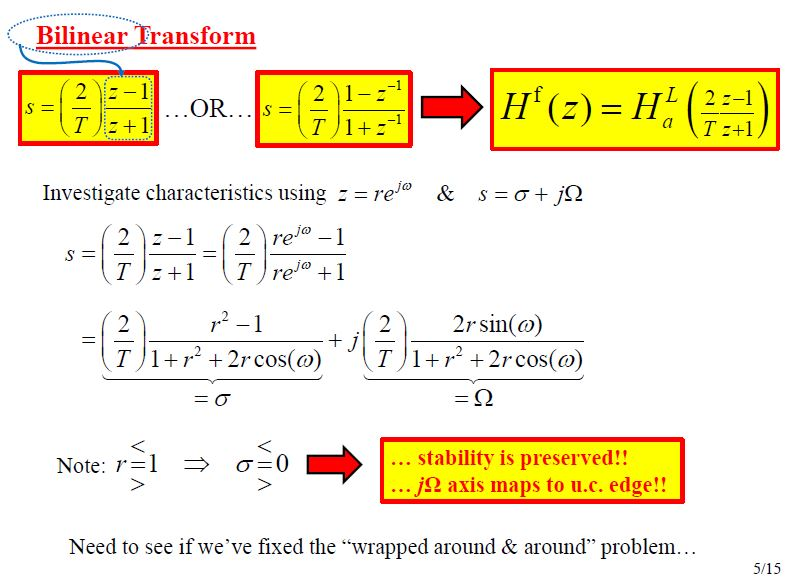
\includegraphics[width = 0.7\textwidth, frame]{Figures/IIR/proof_mapping}
\caption{Proof of Mapping}
\label{fig:IIR:proof_mapping}
\end{figure}

Concerning this proof, it isn't very clear how the researcher start with it or what is the motivation behind it, but it works.\\

Now the next step is to set $r \, = \, 1$ and $\sigma \, = \, 0$, so we can at the circle and the LHP of the $s$-plane, plugging in these values in \autoref{Eq:IIR:2nd_mapping} we get:

\begin{equation}
    \omega \, = \, 2 \, \tan^{-1} \left (\, \displaystyle\frac{\Omega \, T}{2}   \,\right)
    \label{Eq:IIR:freq_mapping}
\end{equation}

\newpage
An example of \autoref{Eq:IIR:freq_mapping} is shown in \autoref{fig:IIR:Warping_frequencies_effect}.

\begin{figure}[h]
\centering
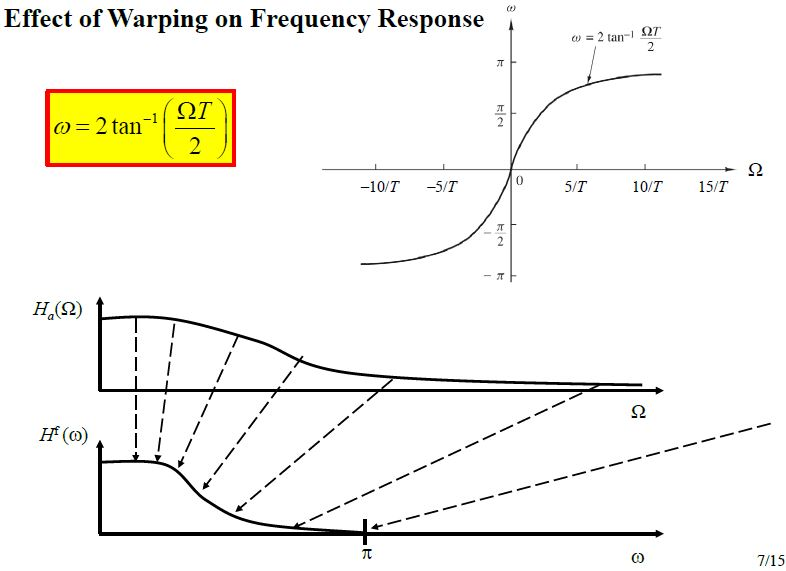
\includegraphics[width = 0.7\textwidth, frame]{Figures/IIR/Warping_frequencies_effect}
\caption{Effect Of Warping frequencies}
\label{fig:IIR:Warping_frequencies_effect}
\end{figure}

We can see that the continuous transfer function $H(\Omega)$ is spread out over all $\Omega$, and then the discrete transfer function $H(\omega)$ is squish to $\pi$, and this compression is controlled by $T_s$.

The higher the $T_s$, the more compression we get.




\chapter{Multirate Signal Processing}

\section{Reference Used}

Chapter 12 from \cite{book_Li_Tan_dsp_fundamentals_and_app}, and chap from \cite{DSP_DimitrisManolakis}.


\section{Downsampling}

We will see now what happen when we do sampling at $T_s$ then do downsampling at a rate of $M \, T_s$ (downsample)


\begin{figure}[h]
\centering
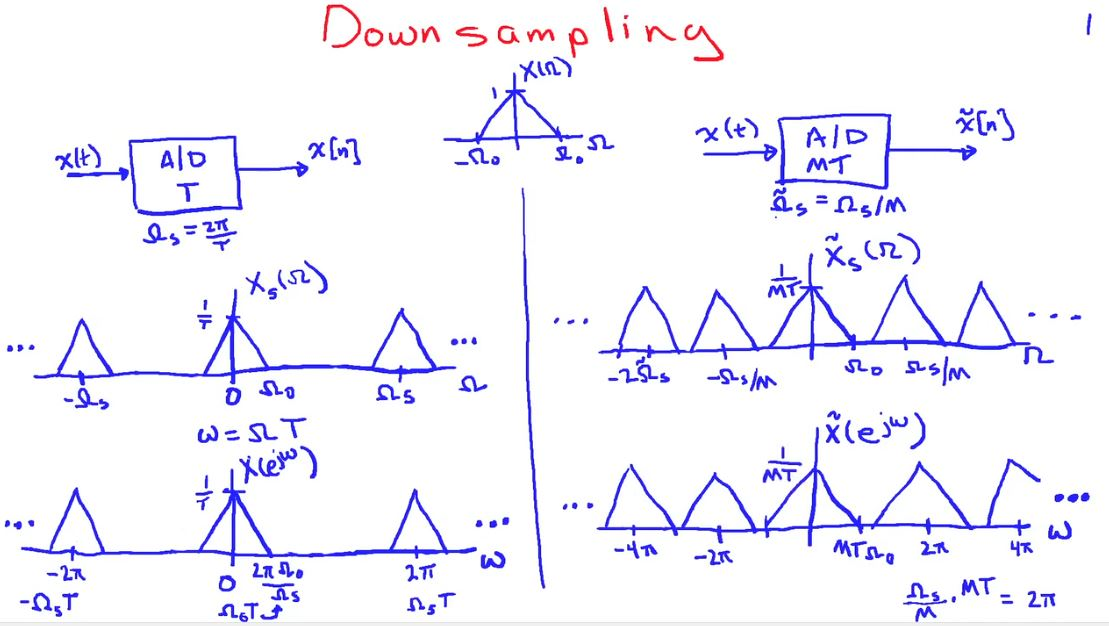
\includegraphics[width = 0.7\textwidth, frame]{Figures/Multirate/downsampling}
\caption{Downsampling effect in the frequency domain}
\label{fig:Multirate:downsampling}
\end{figure} 

\begin{itemize}

\item At a rate of $T_s$, the spectrum get replicated at a multiple of $\omega_s$.

	\begin{itemize}
	\item When we do the frequency mapping $\omega_d \, = \, \omega_c \, \times \, T_s$, the spectrum get replicated at a multiple of 2 $\pi$
	
	
	
	\end{itemize}

\item When doing downsampling:

	\begin{itemize}
	\item $T_{\text{downsample}} \, = \, M \, \times \, T_s$ where $M \, > \, 1 \in \, \mathbb{N}$ and $\omega_{\text{downsample}} \,= \, \displaystyle\frac{\omega_s}{M}$
	
	
	\item The mapping now in frequency is $\omega_d \, = \, \omega_c \, \times \, T_{\text{downsample}}$
	
	
	\item The frequency spectrum in $\omega_c$ now is getting shifted at a multiple of $\displaystyle\frac{\omega_s}{M} $
	
	
	\item In the discrete domain of $-  \pi \, \leq\omega_d \, \leq \,  \pi$, the amplitude is scaled down by $\displaystyle\frac{1}{M \, T_s}$ and the bandwidth is expanded by a factor of $M \, T_s$
	\end{itemize}


\item Aliasing:

If the signal to be downsampled (that is the original signal) has frequency components larger than the new folding frequency $ \leftrightarrow \, f \, > \, \displaystyle\frac{f_s}{2 D}$
aliasing noise will be introduced into the downsampled data.


    \begin{itemize}
        \item To avoid aliasing, the anti-aliaising filter should have a stop frequency edge at $\displaystyle\frac{f_s}{2 \, D}$ (or $\displaystyle\frac{\pi}{D}$ radian in discrete frequency)
    \end{itemize}





\end{itemize}




\subsection{Implementing Downsampling}


\begin{figure}[h]
\centering
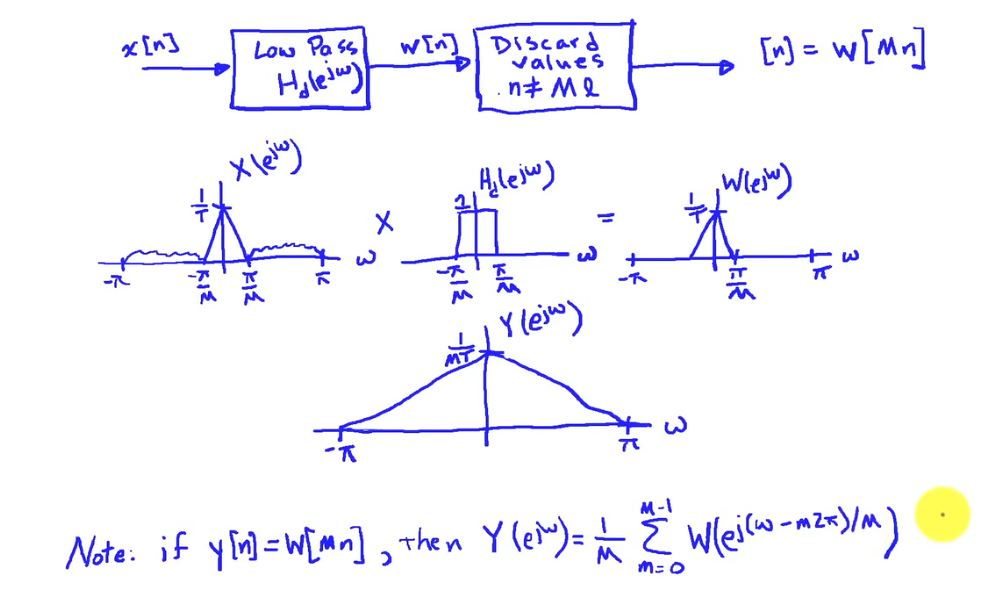
\includegraphics[width = 0.7\textwidth, frame]{Figures/Multirate/implementing_downsampling}
\caption{Implementation of downsampling}
\label{fig:Multirate:implementing_downsampling}
\end{figure} 


\begin{enumerate}

\item Input the discrete signal $x[k]$ in a low pass filter to prevent aliasing 


\item Then we throw the values that are not multiple of $M$

	\begin{itemize}
	\item $y[k] \, = \, w \left[M \, k \right]$: scaling the discrete time axis by a factor of $M$
	
	
	\item We compress the signal in time which means we stretch it in frequency domain: the amplitude spectrum of the signal has stretch out from $\displaystyle\frac{\pi}{M} \, \rightarrow \, \pi$
	
	\item DTFT property for scaling:
	
	
	if $y[k] \, = \, w \left[M \, k \right] \, \rightarrow \, Y(\omega_d) \, = \, \displaystyle\frac{1}{M} \, \displaystyle\sum\limits_{m  \, = \, 0}^{M \, - \, 1} W \left[\, \text{exp}\, \left(\, \displaystyle\frac{j \left(\, \omega_d \, - \, m \, 2 \, \pi \,\right)}{M} \, \right)  \,\right]$
	\end{itemize}


\end{enumerate}

\newpage
\section{Upsampling}

Upsampling is also know as discrete time interpolation.

Effect on spectrum both in continuous time frequency and discrete time frequency is shown in \autoref{fig:Multirate:upsampling}.

\begin{figure}[h]
\centering
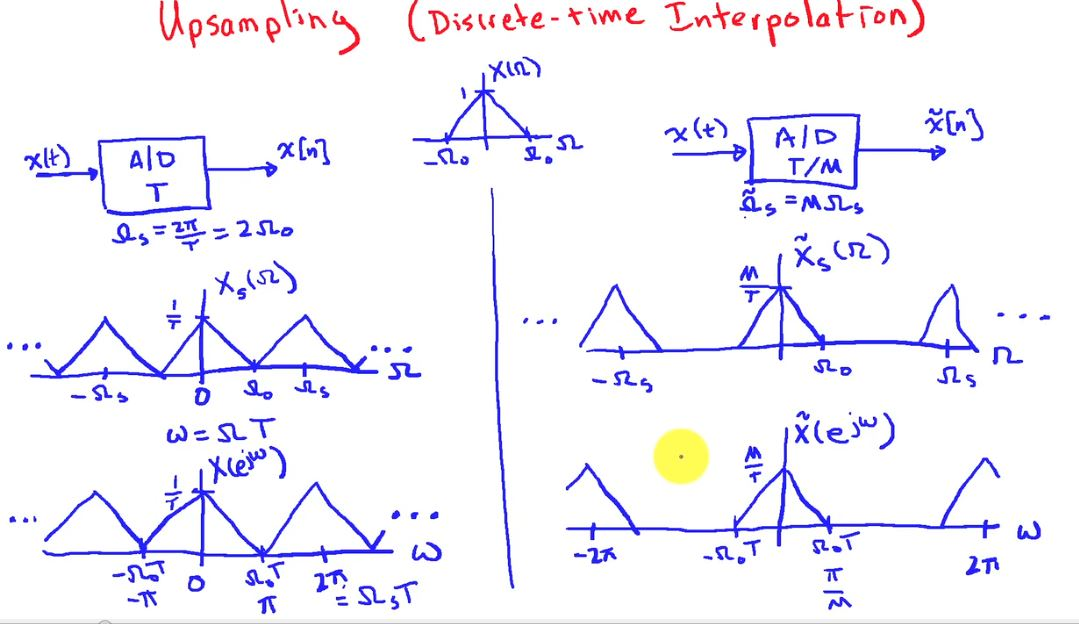
\includegraphics[width = 0.7\textwidth, frame]{Figures/Multirate/upsampling}
\caption{Upsampling effect in the frequency domain}
\label{fig:Multirate:upsampling}
\end{figure} 

\begin{itemize}

\item Opposite to downsampling operation, upsampling compress the spectrum 

\end{itemize}

Example of upsampling in discrete time domain is shown in \autoref{fig:Multirate:upsampling_example}.

\begin{figure}[h]
\centering
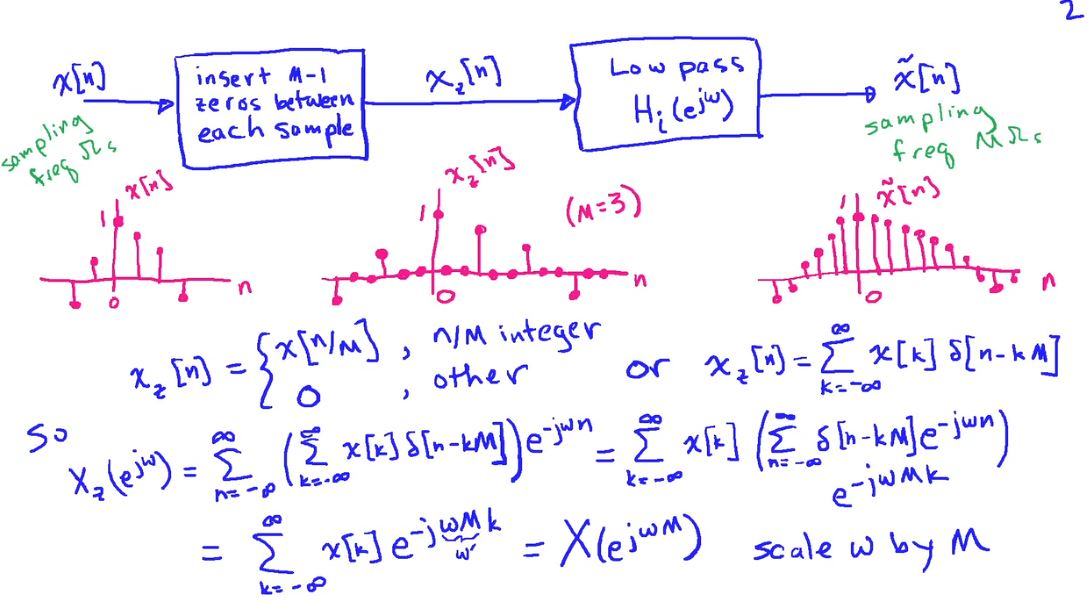
\includegraphics[width = 0.7\textwidth, frame]{Figures/Multirate/upsampling_example}
\caption{Upsampling Example}
\label{fig:Multirate:upsampling_example}
\end{figure} 

\begin{itemize}

\item We add 0 between each sample of the original discrete time $x(k)$ signal such that $\displaystyle\frac{n}{M} \in \mathbb{N}$

\item Then we filter the signal by a low pass filter

\end{itemize}


\newpage
Example of the process in the DTFT spectrum is shown in \autoref{fig:Multirate:upsampling_example_spectrum}.

\begin{figure}[h]
\centering
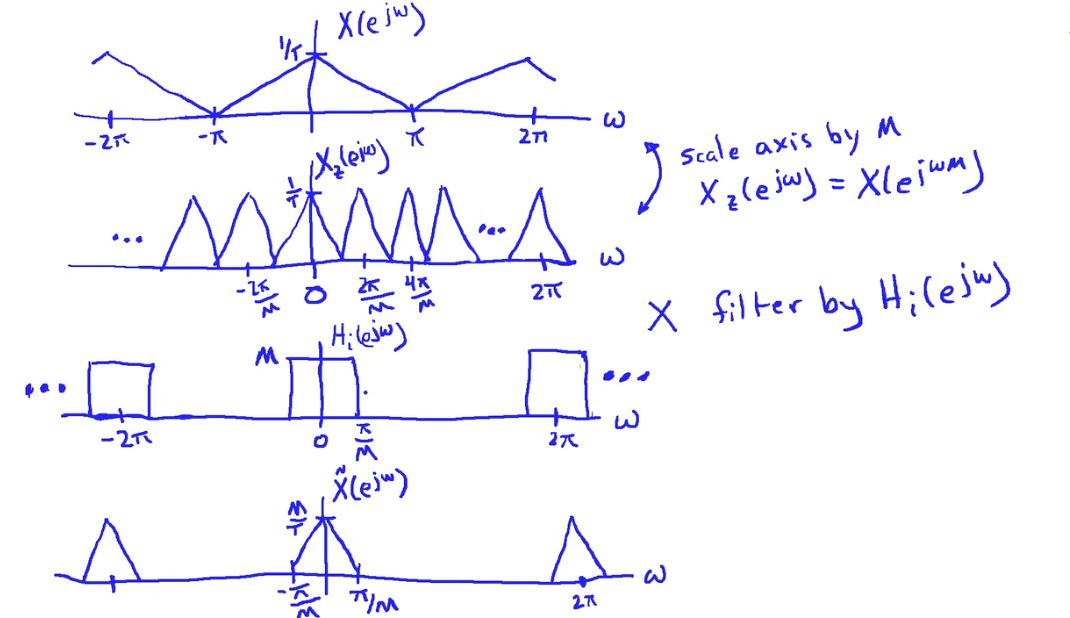
\includegraphics[width = 0.7\textwidth, frame]{Figures/Multirate/upsampling_example_spectrum}
\caption{Upsampling Example in DTFT spectrum}
\label{fig:Multirate:upsampling_example_spectrum}
\end{figure} 


\begin{itemize}

\item The spectrum at $\pi$ in $X(\omega_d)$ is now shown at $\displaystyle\frac{\pi}{M}$ in $X_z(\omega_d)$ 

\item We filter the signal $X_z(\omega_d)$ using a LPF 

\end{itemize}

%*****************************************************
%*****************************************************
%*****************************************************

\chapter{Multirate Sampling by Dr.Michael Lustig Berkely}


\section{Motivation}



\section{Downsampling}


\begin{itemize}

\item The input of the dowsampling operation is a discrete signal $x[k]$

\item What happens when we do dowsampling ?

The answer is in the spectrum.

\begin{itemize}
\item Recall that sampling in time give us replicate in frequency

\item DTFT for $x[k]$ and $x_{\text{decimated}}[k] \, = \, x[k \, M]$ where $M$ is the dowsampling factor


\item Equations:

\begin{equation}
\begin{array}{rcl}
X(\omega_d) \, &=& \, \displaystyle\frac{1}{T_s} \, \displaystyle\sum_n X_c \left[\, j \, \left(\, \omega_d \, - \, n \, \omega_s \,\right)  \,\right] \\ \\
X_{\text{decimated}}(\omega_d) \, &=& \, \displaystyle\frac{1}{M \, T_s} \, \displaystyle\sum_n X_c \left[\, j \, \left(\,  \displaystyle\frac{\omega_d}{M}  \, - \, n \,  \displaystyle\frac{\omega_s}{M} \,\right)  \,\right] 
\end{array}
\label{Eq:Multirate_Sampling_Decimation_spectrum_relation}
\end{equation}

Equation (\ref{Eq:Multirate_Sampling_Decimation_DTFT}) says that if we compress in time, we get more replicate in the frequency


\end{itemize}

\item Next step: is to find the relation between $X_{\text{DTFT}}(\omega_d) $ and $X_{\text{decimated}}(\omega_d) $ without using the CTFT spectrum $X_{\text{CTFT}}(\omega_c)$
	
	\begin{itemize}
	\item Relation:
	
	\begin{equation}
	\begin{array}{rcl}
		X_{\text{decimated}}(\omega_d) \, &=& \, \displaystyle	\frac{1}{M} \, \displaystyle\sum_{i \, = \, 0}^{M \, - \, 1} X_{\text{DTFT}} \left(\,  \displaystyle\frac{\omega_d}{M} \, - \, \displaystyle\frac{2 \pi}{M} \, i \,\right)   
	\end{array}	\label{Eq:Multirate_Sampling_Decimation_spectrum_dtft_relation}
	\end{equation}		
	
	\item Equation (\ref{Eq:Multirate_Sampling_Decimation_spectrum_dtft_relation}) tells us that our bandwidth will expand (stretch) by a factor of $M$.

	\end{itemize}


\end{itemize}



\section{Aliasing Revisited}

Recall that in aliasing , if we have $f \geq \, \displaystyle\frac{F_s}{2}$, then aliasing.\\

In undersampling (1 of Bandpass Sampling techinques:)

\begin{itemize}
    \item Rule: The sampled spectrum must fall in a 1 Nyqyuist Zone only
\end{itemize}


%\begin{figure}[h]
%\centering
%\includegraphics[width = 0.7\textwidth, frame]{Figures/Multirate/undersampling_Nyquist_zone}
%\caption{Upsampling Example in DTFT spectrum}
%\label{fig:Multirate:undersampling_Nyquist_zone}
%\end{figure} 

\underline{Note:} figure undersampling Nyquist zone not found


\section{Upsampling}

So much like digital to analog conversion (to a certain point they have similarities, but not the same).



% **************** References ****************

\bibliographystyle{IEEEtran}

\bibliography{Literature/Books_Signal_Processing,Literature/Papers_Signal_Processing}

\end{document}


